\chapter{\acs{lidar} Interference}
\label{chapter:lidar-interference}

\ac{lidar} interference occurs when the signal of one \ac{lidar}, ``A'', interferes with the signal of another \ac{lidar}, ``B'', affecting its measurements, i.e., \ac{lidar}'s ``B'' capability to measure the distance is not independent of the presence of another \ac{lidar} on its surroundings. In telecommunications, when two devices on the same channel or physical environment interact, creating an undesirable effect with negative consequences, we are in the presence of crosstalk. In a \ac{lidar} interference scenario, this interference can be direct or indirect (the beam is reflected on other surface(s) before hitting \ac{lidar} ``B'') and is a crosstalk phenomenon between the two \acp{lidar}.

The main goal of this thesis is to study the \ac{lidar}'s interference behaviour, expanding the previous work, presented in Section~\ref{sec:sota:lidar-interference}. \acl{sota} in \ac{lidar} interference is still reduced, with the major contributions from only two research teams (Gunzung Kim\etal~\cite{Kim2015c, Kim2017} and Gerald Popko\etal~\cite{Popko2019a, Popko2019b}), both using only two-dimensional \acp{lidar}, i.e., rotating \acp{lidar} that can scan a single line of the scene.

On this chapter, we start by explaining the additions to the previously described experimental setup, in Section~\ref{sec:calibration:experimental-setup}, that allows us to investigate the impact of several parameters on \ac{lidar} interference behaviour. Test scenarios are detailed and the test conditions under which data was acquired are explained. Since one of the thesis objectives, detailed in Section~\ref{sec:introduction:objectives}, is to create a comprehensive experimental dataset with different metrics for future tests on \ac{lidar} interference, we describe how the experimental dataset was organized to ensure it could be easily reused and also to streamline data analysis in this study.

Our first \ac{lidar} interference analysis results are obtained from Bosch\cp~datasets, allowing a qualitative assessment of the interference. Based on these results, we sought to explain this behaviour by quantifying the number of outliers that have no physical context on the data, such as points below ground or outside a closed room dimensions.

To provide a more in-depth analysis of the interference, a comparison with a ground-truth model of the test environment is required. We propose two methods to generate such ground truth model from the data without interference. Using these models, we also propose two methods to measure the interference, unveiling their algorithms and results.

Following up on the outcomes provided by Chapter~\ref{chapter:object-detection}, we apply the previous algorithms onto the selected \acp{roi} on the point cloud, that correspond to the bounding boxes of image objects previously detected on the image, using the calibration notions gathered from Chapter~\ref{chapter:calibration}.

Lastly, we conclude our findings and compare them with the current \acl{sota} on \ac{lidar} interference.

%%%%%%%%%%%%%%%%%%%%%%%%%%%%%%%%%%%%%%%%%%%%%%%%%%%%%%%%%%%%%%%%%%%%%%%%%%%%%%%%%%%%%%%%%%%%%%%%%
%%%%%%%%%%%%%%%%%%%%%%%%%%%%%%%%%%% EXPERIMENTAL SETUP %%%%%%%%%%%%%%%%%%%%%%%%%%%%%%%%%%%%%%%%%%
%%%%%%%%%%%%%%%%%%%%%%%%%%%%%%%%%%%%%%%%%%%%%%%%%%%%%%%%%%%%%%%%%%%%%%%%%%%%%%%%%%%%%%%%%%%%%%%%%


\section{Experimental Setup}
\label{sec:lidar-interference:experimental-setup}

Expanding the previous experimental setup, detailed in Section~\ref{sec:calibration:experimental-setup}, requires adding another \ac{lidar} for acting as an interferer. This \ac{lidar} is mounted on a tripod and serves the purpose of interfering with the measurements of the first \ac{lidar}, already present on the earlier version of the experimental setup (see Figure~\ref{fig:experimental-setup}), which becomes its ``victim''\footnote{The terms victim and interferer, when referring to \ac{lidar} interference, are first connoted by Gunzung Kim\etal on~\cite{Kim2015a, Kim2015b, Kim2015c, Kim2017}, and later adopted by Gerald Popko\etal~\cite{Popko2019a, Popko2019b}. To keep the notation coherent with the \acl{sota}, we will use the same denominations on this chapter.}.

The interferer \ac{lidar} is a HESAI\cp~Pandar40\texttrademark, a 40 beams \ac{tof} rotating \ac{lidar} that operates at a wavelength of \SI{905}{\nano\meter}. Pandar40 supports various measurement modes based on the return pulse (Strongest, Last, Dual) and can be connected to a \ac{gps} receiver for geopositioning and synchronization with an external clock. It also supports two rotation velocities: 600 or 1200 \ac{rpm}, which result in different angular steps and point cloud refresh rate. 

Pandar40's \ac{lidar} has an asymmetrical vertical \ac{fov}, varying from \SIrange{-16}{+7}{\degree}. A larger channel density occurs between the angles \SI{-6}{\degree} and \SI{+2}{\degree}, with 25 pairs of lasers and photodetectors with \SI{0.33}{\degree} apart from each other. From \SIrange{-16}{-6}{\degree} and \SIrange{+2}{+7}{\degree}, the angular step between the pairs of lasers and photodetectors is \SI{1}{\degree}, and only 15 pairs of lasers and photodetectors are used: 5 above and 10 below.

The full specifications of the HESAI Pandar40 can be accessed on~\cite{Pandar40UserGuide} and the relevant specifications for this work are summarized in Table~\ref{tab:pandar40-specs}.

\begin{table}[!ht]
\centering
\renewcommand{\arraystretch}{1.2}
\rowcolors{3}{gray!10}{white}
\begin{tabular}{@{}p{6cm}c@{}}
	\toprule
	Specifications & Value \\
	\midrule
	Wavelength & \SI{905}{\nano\meter} \\
	Motor \ac{rpm} & 600 \\
	Angular Step & \SI{0.2}{\degree} \\
	Vertical \ac{fov} & \SI{23}{\degree} \\
	Horizontal \ac{fov} & \SI{360}{\degree} \\
	Maximum Scanning Distance & \SI{200}{\meter} @20\% reflectivity \\
																				 & $\pm \SI{5}{\centi\meter}$, from \SIrange{0.3}{0.5}{\meter} \\
	\rowcolor{white} \multirow{-2}{*}{Measurement Accuracy} & $\pm \SI{2}{\centi\meter}$, from \SIrange{0.5}{200}{\meter} \\
	\bottomrule
\end{tabular}
\caption[HESAI Pandar40 relevant specifications.]{HESAI Pandar40 relevant specifications. Source~\cite{Pandar40UserGuide}.}
\label{tab:pandar40-specs}
\end{table}

The tripod used for the experimental setup is a Velbon\cp~CX-460\texttrademark~tripod, that also has a central monopod. For increased stability on the measurement procedure, the monopod was never used. The tripod ranges in height from approximately \SIrange{0.62}{1.28}{\meter}, measured from its feet to its basis. Since the tripod used is a camera tripod, a gimmick must be done to ensure proper fixation of the Pandar40 \ac{lidar}, by replacing the universal camera support bolt with an \SI{12}{\milli\meter} length M6 bolt, tightened with an M6 nut and two metal rings. The Pandar40, secured on the tripod is shown in Figure~\ref{fig:pandar40-on-tripod}.

\begin{figure}[!ht]
\centering
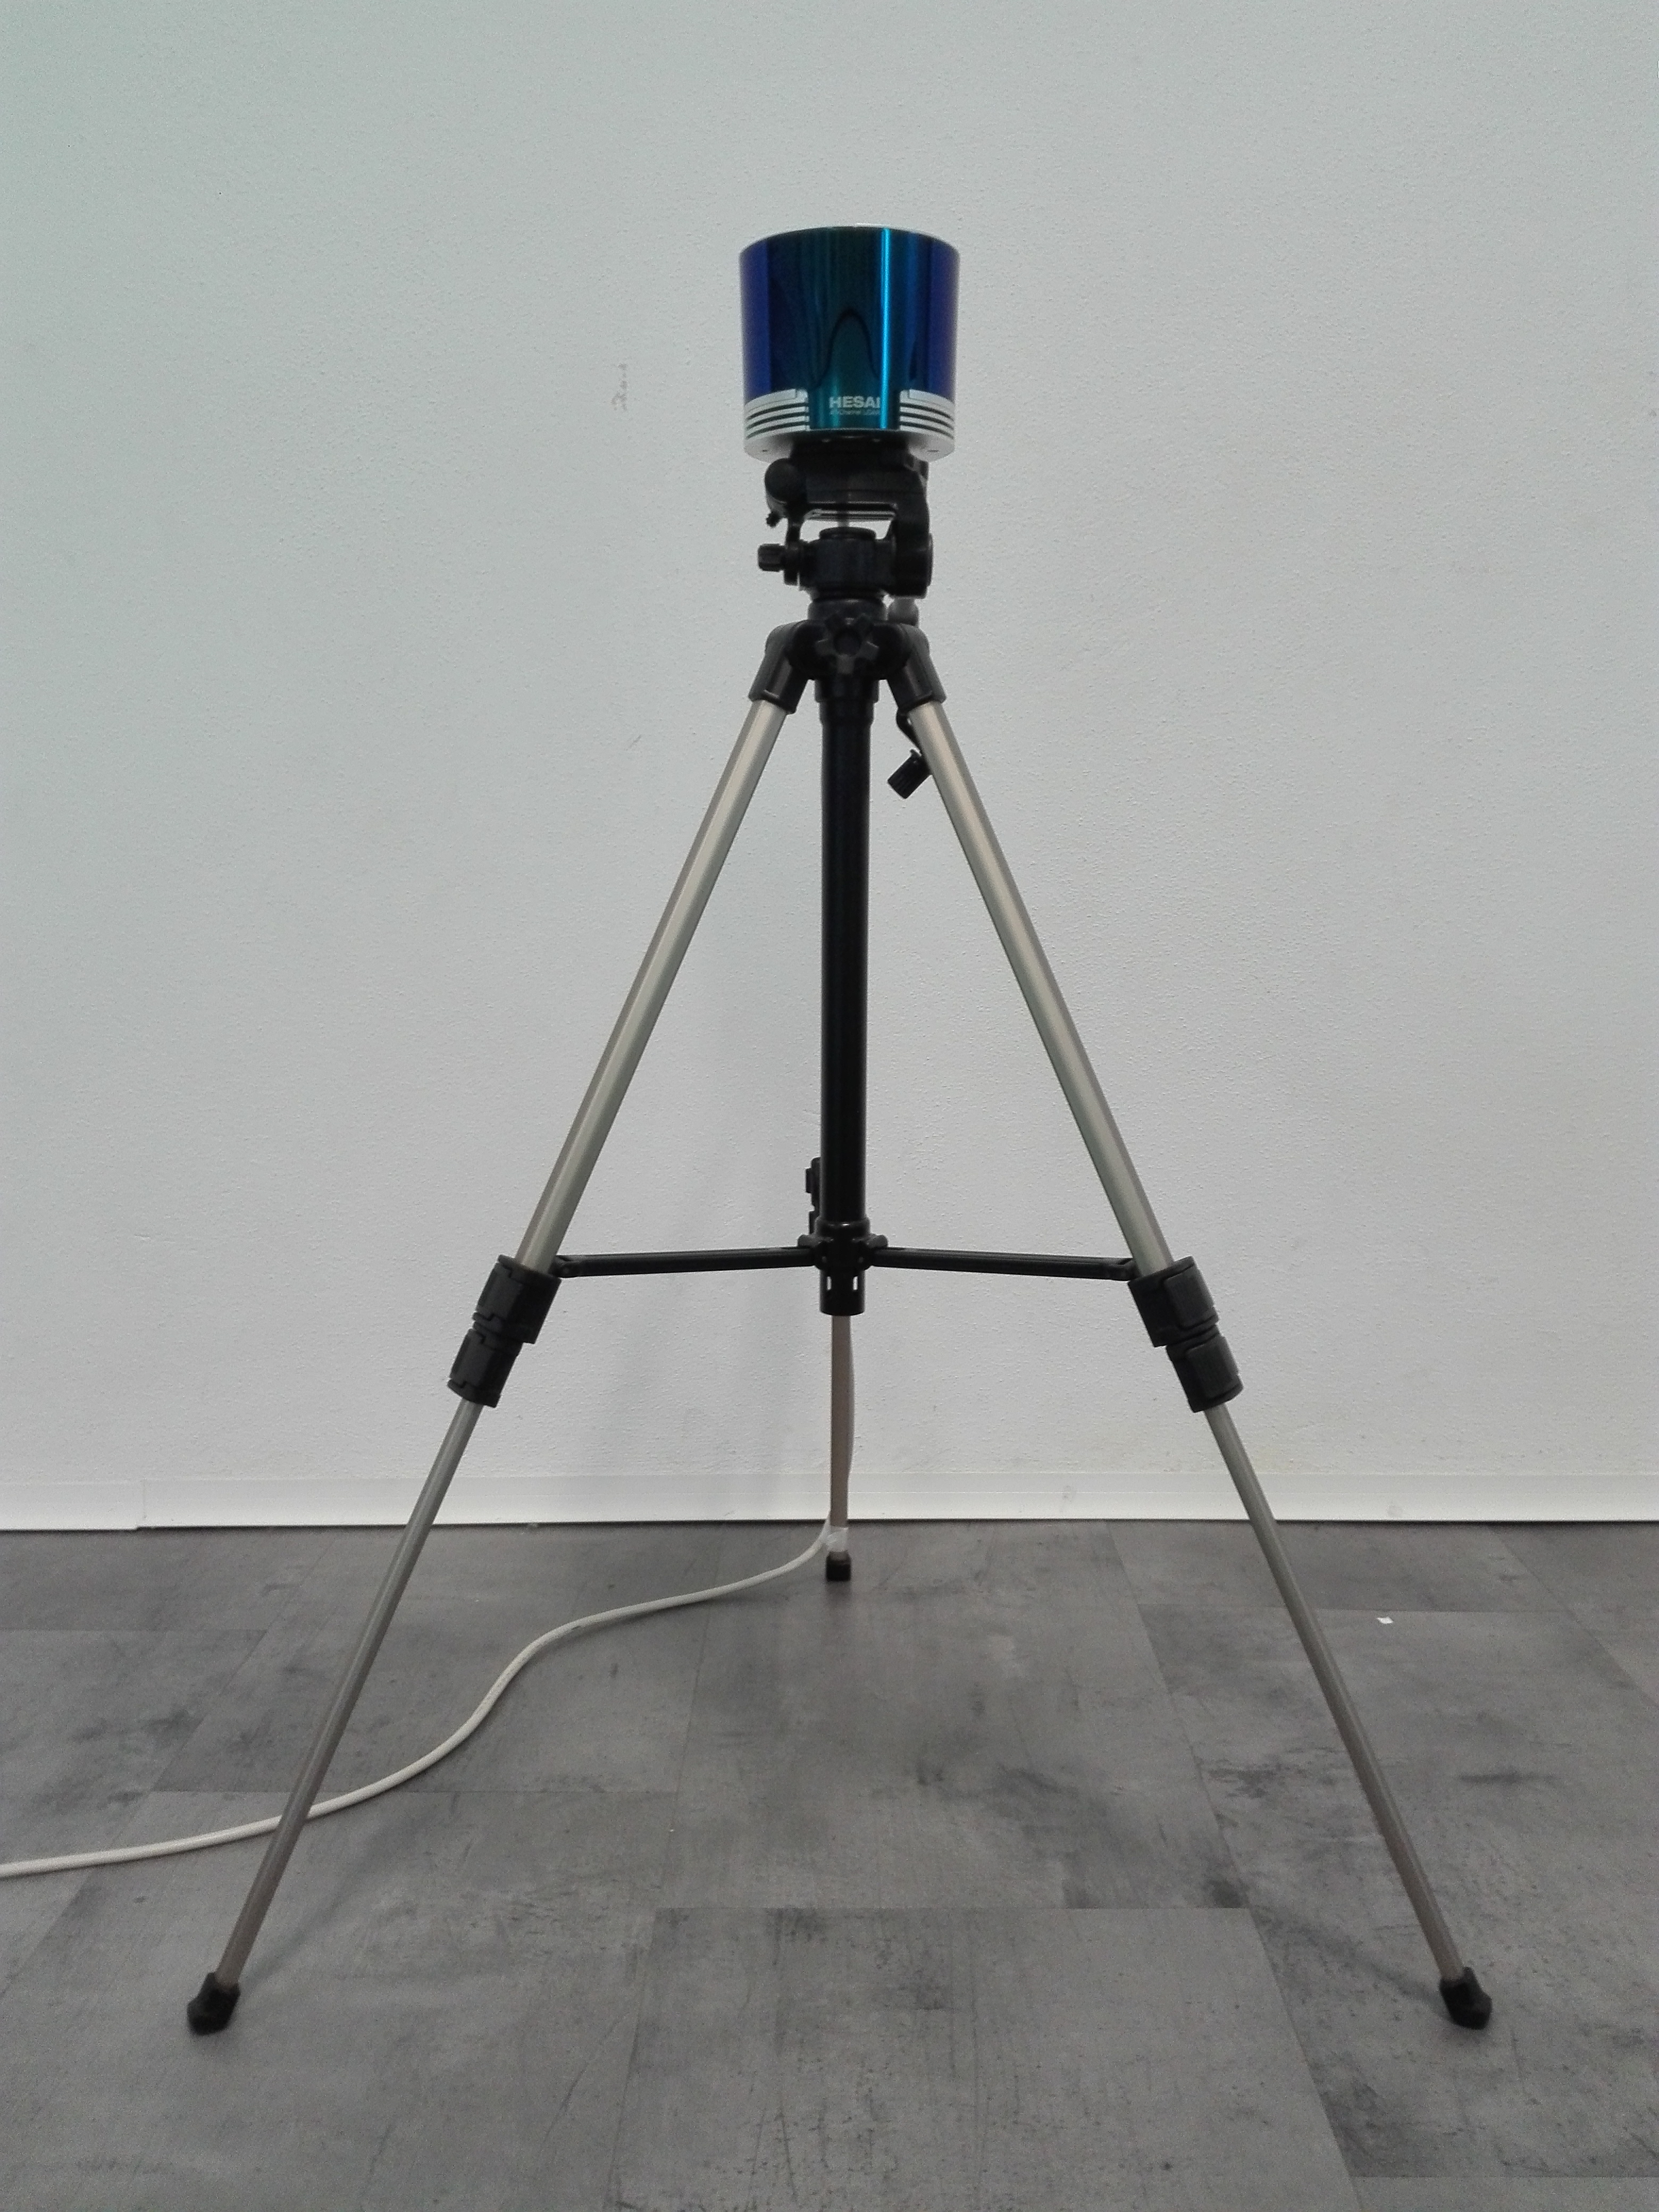
\includegraphics[width=0.4\textwidth]{img/experimental-setup/pandar40-on-tripod.jpg}
\caption[HESAI Pandar40 \ac{lidar} on a Velbon CX-460 tripod.]{HESAI Pandar40 \ac{lidar} on a Velbon CX-460 tripod.}
\label{fig:pandar40-on-tripod}
\end{figure}

Despite the two \acp{lidar}'s laser nominal wavelengths being slightly difference, no majors drawbacks are expected due to the mismatch, due to wavelength shift caused by the operating temperature and that the \ac{ir} filter used as a bandwidth of, at least, \SI{10}{\nano\meter}. Velodyne's VLP-16, the victim, operates at \SI{903}{\nano\meter} and HESAI Pandar40, the interferer, operates at \SI{905}{\nano\meter}. Ideally, the same \ac{lidar} model would be used for the victim and interferer, but such material was not available. Nevertheless, we are unable to easily predict how the different number of channels, asymmetric channel distribution, variable angular step and different laser wavelength will impact the interference behaviour, due to the lacking of prior knowledge available on the area. Such study is out of the focus of this study and is left for future work.

\subsection{Experimental Test Scenarios}
\label{subsec:lidar-interference:test-scenarios}

Two locations were used as test scenarios for \ac{lidar} interference: Aveiro's \ac{it} Dark Room and \ac{irislab} \ac{msl} robotic soccer field. At the former, acquaintance with the experimental setup, calibration procedures and tests to gathered preliminary knowledge on \ac{lidar} interference were carried. At the latter, experimental tests were devised to assess the impact of relevant parameters under study on \ac{lidar} interference. 

Aveiro's \ac{it} Dark Room is an optical laboratory that is capable of blocking all external light (hence its name). It measures $\SI{5.20}{\meter} \times \SI{6.97}{\meter} \times \SI{2.80}{\meter}$ and is equipped with benchtop, chairs, optical experimental setup, among other things, creating a rich scenario for a \ac{lidar} rangefinder. 
\ac{irislab} \ac{msl} robotic soccer field measures $\SI{18.0}{\meter} \times \SI{11.5}{\meter}$ and is placed inside \ac{irislab} building, a research facility whose main division has $\SI{34.346}{\meter} \times \SI{16.097}{\meter} \times \SI{4.289}{\meter}$, if measured to the ceiling and not the ceiling girders. 

All distance measures presented in this Chapter are taken using a LOMVUM LV66V \SI{80}{\meter} handheld laser rangefinder, which is used in this context as the distance calibration instrument. When taking measures, the orientation of the rangefinder was kept in the interval of $[\SI{-0.2}{\degree}, \SI{0.3}{\degree}]$. The error associated to each laser measurement, according to LOMVUM datasheet\footnote{No online manual was found. Measurement error determined by consulting the product printed datasheet, supplied with the device.} is \SI{1.5}{\milli\meter}. To minimize the error introduced by the human operator, 10 measurements were done and their average was taken using the LOMVUM's laser rangefinder capabilities.


\subsection{Parameters under study}
\label{subsec:lidar-interference:parameters-under-test}
On \ac{irislab}, several tests were devised to tackle the problem of \ac{lidar} interference from different perspectives. Test scenarios were carried, where only one parameter is varied, in an attempt to understand the interference behaviour between data. The test parameters under study, from which different datasets were recorded are:

\begin{itemize}
	\item \textbf{Distance between \acp{lidar}:} Keeping the \acp{lidar} azimuthal origin aligned and with their optical axis at the same height, the distance between the interferer and victim is changed, by moving the interferer further away. The distance between the two was varied in steps of \SI{1}{\meter}, from \SIrange{1}{12}{\meter};
\item \textbf{Height:} To evaluate the impact of the elevation angle, for a fixed distance between the two \acp{lidar}, with its azimuthal origin aligned, the height between the two is varied in non-uniform steps, from \SIrange{0.623}{1.277}{\meter} measured in relation to the floor, which results in \SIrange{-0.295}{0.359}{\meter} when compared with the victim \ac{lidar} height;
\item \textbf{\acp{lidar} \ac{los} obstruction:} To quantify the impact of direct and indirect interference, an obstacle is placed on the \acp{lidar} \ac{fov}, breaking the \ac{los} between the two \acp{lidar}. This test scenario is similar to that of the Distance tests, but places the obstacle at the middle distance between the victim and interferer \ac{lidar}. The measurements were carried out only when the distance between the interferer and the \ac{lidar} was an even number.
\item \textbf{Rotation Speed:} To measure the impact of different rotation speeds between the \acp{lidar}, the victim's \ac{lidar} is kept at the same rotation speed as the other tests, while the interferer \ac{lidar} rotation speed is changed. Distance is constant, the \ac{lidar}'s azimuthal origin is aligned and their optical axis is at the same height;
\item \textbf{Orientation:} To study the interference directionality, the relative angular position between the victim's and the interferer \ac{lidar} is changed, while keeping their optical axis at the same height and the same distance for all variations of this parameter.
\end{itemize}


\subsection{Dataset Organization}
A thesis objective on its own (see Section~\ref{sec:introduction:objectives}), dataset organization is a crucial for a proper data analysis. With 5 parameters under test, each with several values, 60 different interference test exists, in addition to camera calibration data and data without interference. In total, more than \SI{600}{\giga\byte} of pre-processed raw data, ready to be analyzed, is stored, in a total of almost 180 \ac{ros} bag files, totalling almost 4 hours and 20 minutes of playable data. Several hundred files, among camera calibration, rigid body transformation and results, are also contained in the dataset structure, for a total of more than \SI{1}{\tera\byte} of data and results.

A comprehensive diagram that details the dataset directory and file tree hierarchy for data recording is given on~\nameref{appendix:datasets-tree}. The \textit{Experimental Datasets} folder is the root folder of the data, containing the two test locations, \textit{IRIS Laboratory} and \textit{IT2 Dark Room}. 

The standardization of test scenarios started at \ac{it} 2 Dark Room, but only matured at \ac{irislab}. This standardization forces guidelines on file and folder naming, directory structure organization and data to record. On every folder, a \textit{README.md} file is present, detailing the files and/or folders in its hierarchy level, and the test conditions, if applicable. 

At \ac{it} 2 Dark Room, only \textit{Scenario B} follows these guidelines, which were inspired by \ac{kitti}'s dataset~\cite{Geiger2013a}. Since our setups location is fixed, each location defines a root folder for all the tests happening in that location, with its subfolders being the day on which the data was acquired. These type of folders contain  3 subfolders, whose goal is detailed below and an extract of its  hierarchy organization is given in Figure~\ref{fig:test-subfolders}.

\begin{figure}[!ht]
\centering
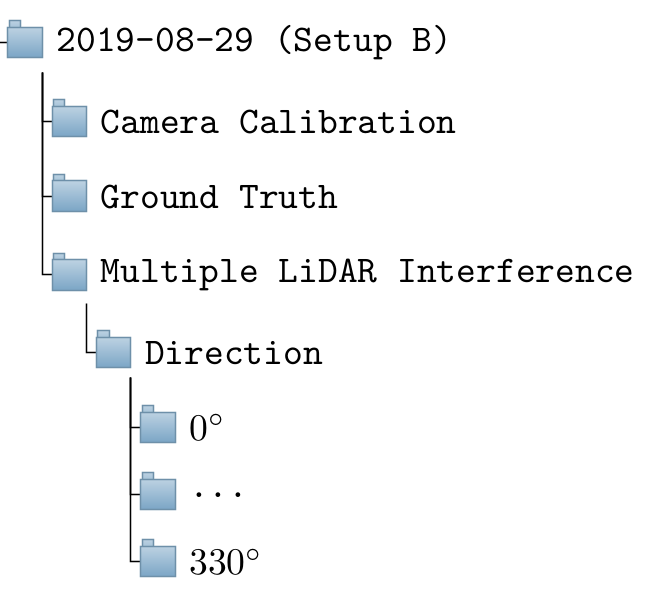
\includegraphics[scale=0.3]{img/datasets/test-subfolders.png}
\caption[Dataset folder hierarchy for a ``test day''.]{Detail of the hierarchy of a ``test day''. On each day data was recorded, calibration and ground-truth data were recorded. \textit{Multiple Lidar Interference} folder contains the parameters under test and each of the tested values.}
\label{fig:test-subfolders}
\end{figure}


\begin{enumerate}
\item \textit{Camera Calibration}: Contains the calibration images, intrinsic calibration parameters, \ac{ros} bag files containing the camera and \ac{lidar} raw and pre-processed data and the log file of the calibration procedure;
\item \textit{Ground Truth}: One or more \ac{ros} bag file containing the static scenario, without objects of interest placed on the camera and \ac{lidar}'s \ac{fov} and without \ac{lidar} interference;
\item \textit{Multiple LiDAR Interference}: This folder contains a series of subfolders, each for a parameter under test. For each parameter under test folder, subfolders contain the data and results for each of the value that the parameters takes.
\end{enumerate}

On a specific value for a parameter under test, three bag files are present, as shown in Figure~\ref{fig:parameter-test-files}. \textit{interference.bag} is a pre-processed \ac{ros} bag file that contains only \ac{lidar} data with interference. This pre-processing consists on cropping the \textit{original\_raw.bag} file to remove the initial seconds (from \SIrange{20}{30}{\second}), when the interferer \ac{lidar} is still booting up. \textit{ground\_truth} corresponds to data recorded under the conditions of \textit{interference.bag}, but without interference, i.e., the interferer \ac{lidar} is at its position for the test, but switched off.

\begin{figure}[!ht]
\centering
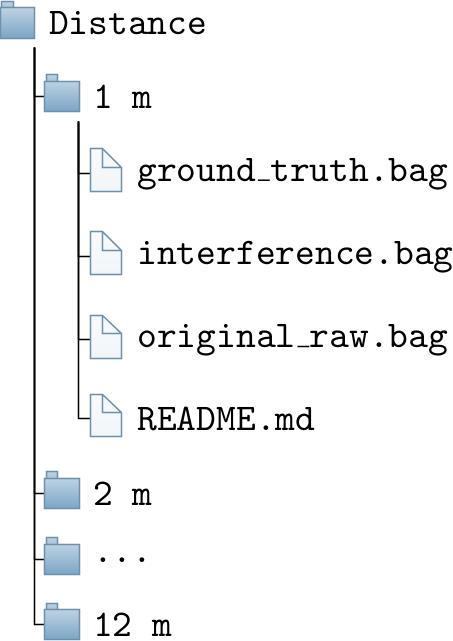
\includegraphics[scale=0.3]{img/datasets/parameter-test-files.png}
\caption[Dataset file hierarchy for a single value of a parameter under test.]{Data recorded using \texttt{rosbag} tool, for a single value of a parameter under test. \textit{README.md}, on this type of folder, details the conditions under which data was gathered.}
\label{fig:parameter-test-files}
\end{figure}


In \textit{IRIS Laboratory} folder, two test folders are present, containing all the data gathered on \ac{irislab}, \textit{2019-08-28} and \textit{2019-08-29}. For each of the folders, different calibration parameters are available, along with ground truths and calibration data. For \textit{\ac{it} 2 Dark Room}, only the data on the folder \textit{2019-07-31} is relevant to interference analysis.

To ease the access to this data structure, \texttt{datasets\_path} library was implemented, both on C++ and Python 3, to allow ubiquitous managing of data loading for tests and saving of results.


%%%%%%%%%%%%%%%%%%%%%%%%%%%%%%%%%%%%%%%%%%%%%%%%%%%%%%%%%%%%%%%%%%%%%%%%%%%%%%%%%%%%%%%%%%%%%%%%%
%%%%%%%%%%%%%%%%%%%%%%%%%%%%%%%%%%%%% BOSCH DATASET %%%%%%%%%%%%%%%%%%%%%%%%%%%%%%%%%%%%%%%%%%%%%
%%%%%%%%%%%%%%%%%%%%%%%%%%%%%%%%%%%%%%%%%%%%%%%%%%%%%%%%%%%%%%%%%%%%%%%%%%%%%%%%%%%%%%%%%%%%%%%%%


\section{Bosch\cp~Dataset}
We start by investigating \ac{lidar} interference using a dataset provided by Bosch. This dataset consists of 3 \ac{ros} bag files, one recorded by a HESAI Pandar40 and two other by Velodyne's VLP-16. Each of the bag files correspond to the same experimental scenario: the two \acp{lidar} are placed, side by side, on top of a table, with the Pandar40 about \SI{50}{\centi\meter} to the left of the VLP-16. For each of the tests, data is recorded for about \SIrange{10}{15}{\second} and the two \acp{lidar} are always switched on.

To analyze the interference, we start by analyze at the data in \texttt{Rviz}, noticing two phenomena: 

\begin{enumerate}
\item Data appears to be more noisy, as if it was oscillating with greater magnitude around a fixed point on its measurement axis, when comparing with \ac{kitti}'s dataset;
\item Some measurements correspond to points outside of the room dimensions.
\end{enumerate}

For the first case, we present two hypotheses: it is caused by the interference of the other \ac{lidar}, or due to the measurements being taken in small rooms. To understand the second phenomenon, a two-dimensional scatter map of the point cloud, viewed from above, is plotted. This representation does not take in consideration the measurement density, which might be misleading, since interfered measurements should have a higher ``geometric'' dispersion and a lower point density when comparing with the correct measurements of the real world.

These results are present in Figure~\ref{fig:bosch-pandar-vs-vlp16}, with the left sub-figure, (\subref{fig:bosch-pandar40}), showing HESAI's Pandar40 data, represented in green, and the right sub-figure, (\subref{fig:bosch-vlp16-1}), showing Velodyne's VLP-16 data, represented in yellow. For each of the sub-figures, we notice in the center a rectangular shape, the room, and the outliers are distributed in a circular arrangement, with preference for some azimuthal angles. The circular range is due to the hardware time window to measure the reception pulse and software distance threshold to register the data. On Pandar40, the software constrain is \SI{200}{\meter} and on VLP-16 is \SI{130}{\meter}. 

Considering the HESAI's \ac{lidar} is left to the Velodyne's \ac{lidar}, the occurrence of interference seem to be more significant to HESAI's right, i.e., between the two \acp{lidar}. On the other hand, Velodyne's outliers tend to its left, the side on which the HESAI's is in. With HESAI's outliers concentrated on its first geometric quadrant and Velodyne's outliers on the second geometric quadrant, such results seem to indicate that interference is directional. However, from this data we cannot determine if this is due to direct interference, reflections or both.

\begin{figure}[ht!]
\centering
\begin{subfigure}[t]{0.45\textwidth}
	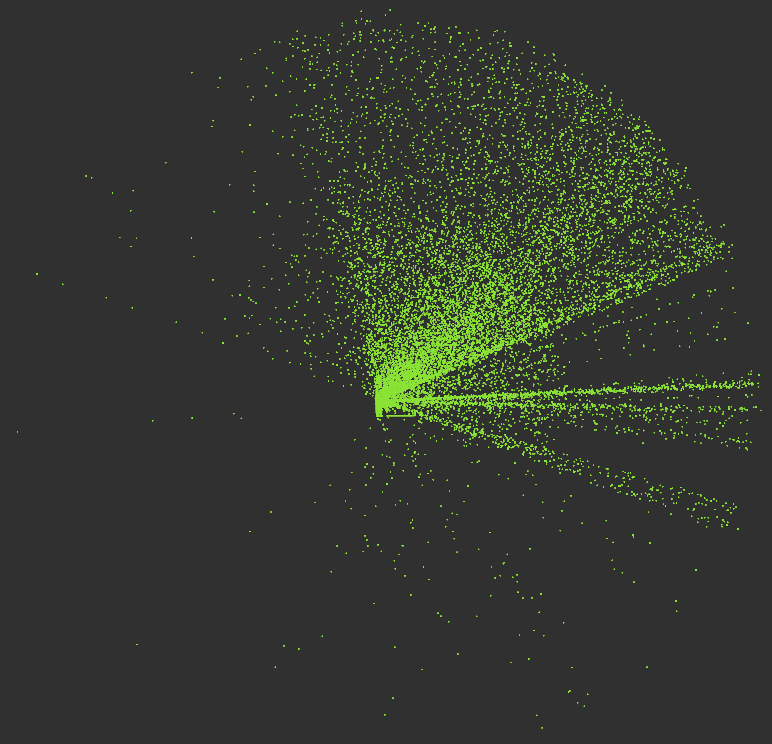
\includegraphics[width=\textwidth]{img/bosch/pandar40.png}
	\caption{HESAI's Pandar40 data scatter plot.}
	\label{fig:bosch-pandar40}
\end{subfigure}
\qquad
\begin{subfigure}[t]{0.45\textwidth}
	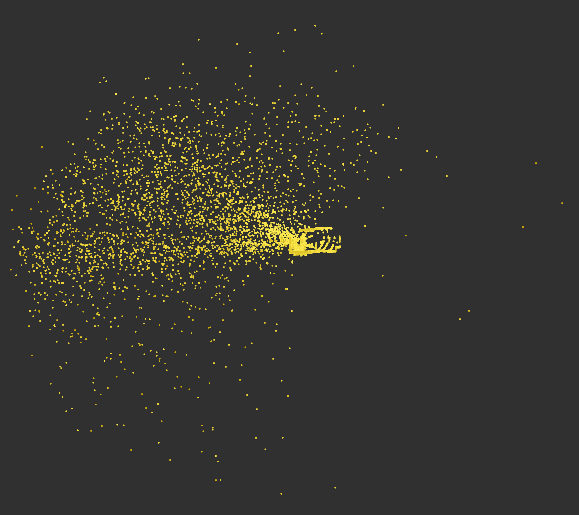
\includegraphics[width=\textwidth]{img/bosch/vlp16-test1.png}
	\caption{Velodyne's VLP-16 data scatter plot}
	\label{fig:bosch-vlp16-1}
\end{subfigure}
\caption[Scatter plot top-view of both \acp{lidar} interference on the dataset provided by Bosch.]{Scatter plot of the data gathered by HESAI's Pandar40, (\subref{fig:bosch-pandar40}), and Velodyne's VLP-16, (\subref{fig:bosch-vlp16-1}). The measurements are plotted only on the X-Y plane, flattening the height of the points.}
\label{fig:bosch-pandar-vs-vlp16}
\end{figure}

We also analyze the results from the second VLP-16 bag file, and compare with the first, in Figure~\ref{fig:bosch-vlp16-comparison}. The previous shown data, in Figure~\ref{fig:bosch-vlp16-1} is shown in yellow and the second dataset in blue. In the center, the room can be seen, and the data, independently of the bag file, seems to have the same dispersion and directionality.

\begin{figure}[ht!]
\centering
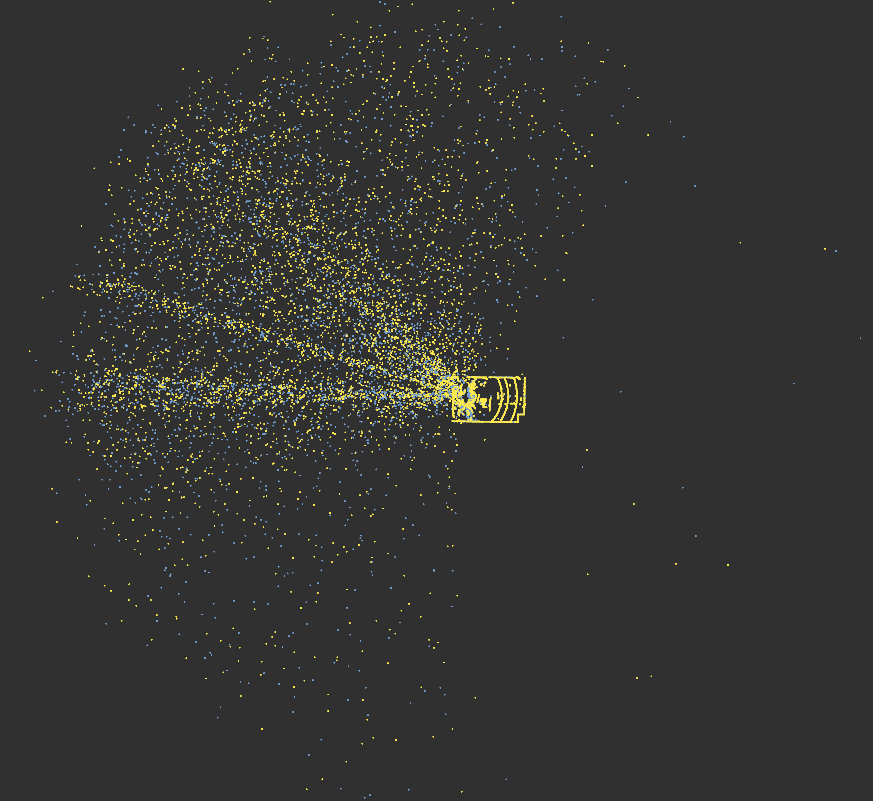
\includegraphics[scale=0.33]{img/bosch/vlp16-tests-overlaid.png}
\caption[Scattered plot of VLP-16 interference taken on two different instants, on the same conditions.]{Scatter plot of the \ac{ros} bags containing Velodyne's VLP-16 data, gathered under the same conditions with almost an hour of difference. Thee measurements are plotted only on the X-Y plane, flattening the height of the points. Comparison between the grid and blue points shows a macro-correspondence.}
\label{fig:bosch-vlp16-comparison}
\end{figure}

Originally, this dataset were not aimed for a detailed analysis on \ac{lidar} interference neither for our approach to study the interference. The sole purpose of such dataset was to illustrate the phenomena of interference. Since the scenario was not static and no data without interference is present, this dataset cannot be used for a refined analysis of the interference, due to the approach and methods we devise suppose that the environment is static, in order for a ground truth model to be generated. Also, no camera is present and therefore, no object detection processing chain can be implemented (similar to Chapter~\ref{chapter:object-detection}). 

Our solution is then to acquire datasets on the conditions described in Section~\ref{sec:lidar-interference:experimental-setup}. For Bosch dataset, we quantize these outliers and try to understand more about their behavior, which is the approach detailed on the next Section.


%%%%%%%%%%%%%%%%%%%%%%%%%%%%%%%%%%%%%%%%%%%%%%%%%%%%%%%%%%%%%%%%%%%%%%%%%%%%%%%%%%%%%%%%%%%%%%%%%
%%%%%%%%%%%%%%%%%%%%%%%%%%%%%%%%%% ROOM OUTLIERS ACCOUNTING %%%%%%%%%%%%%%%%%%%%%%%%%%%%%%%%%%%%%
%%%%%%%%%%%%%%%%%%%%%%%%%%%%%%%%%%%%%%%%%%%%%%%%%%%%%%%%%%%%%%%%%%%%%%%%%%%%%%%%%%%%%%%%%%%%%%%%%


\section{Room Outliers Accounting}
\label{sec:lidar-interference:room-outliers}
After the qualitative analysis of the previous Section on Bosch's dataset, from which we concluded that the \ac{lidar} interference appears to be directional and causes outliers outside of the room dimensions, this Section details the implementation and results of a quantitative approach to analyze the events described on phenomenon 2: \ac{lidar} measurements outside room dimensions.

To analyze the data, a \ac{ros} node, with both offline and online versions, was implemented. Offline operation implies that the node does not have real-time constraints, being capable of handling large \ac{ros} bag files and datasets. The main difference from the online operation, that has been used so far, is that the node does not require another node on the network to publish data for it (typically, a \ac{ros} bag player or a device driver) and the \ac{ros} network does not need to be setup up and running. Instead, the node loads and parses the bag file, as fast as it can or as fast as it is instructed to, keeping its data private on its own program memory. This alternative permits processing large amounts of data and realizing complex analysis on it.

To quantify this interference, the node only needs to know the room dimensions, which we considered to be the majorant and minorant of the room dimensions along each of the 3 Cartesian axes. With it, it can determine the number of point cloud messages received, average number of points per message, absolute and relative number of outliers and inliers. To account for some noise on the data, to the room limits dimensions, a 5\% tolerance is applied. 

An outlier is a point that is not contained within the room dimensions (approximated as a parallelepiped), in all three Cartesian coordinates, considering also the tolerance scaling. Given a point under classification, $P$, and a tolerance, $t$, Equation~\eqref{eq:box-outlier-condition} describes the mathematical decision applied to determine if that point cloud point is an inlier or an outlier.

\begin{equation}
\label{eq:box-outlier-condition}
\begin{cases}
	\begin{aligned}
		\text{inlier}, \qquad \text{if\ } P \in & [\min(x) \cdot t, \max(x) \cdot t] \cup [\min(y) \cdot t, \max(y) \cdot t]  \\
																					&					 \cup [\min(z) \cdot t, \max(z) \cdot t] 
	\end{aligned} \\
	\text{outlier}, \qquad \text{otherwise}
\end{cases}
\end{equation}

Despite this analysis not accounting for the possible interference inside the room dimensions, this interference model intends to measure what, to the ``naked eye'', is clearly an erroneous measure, caused by \ac{lidar} interference: measurements outside the physical dimensions of the room where the \acp{lidar} are located. Since the possible interference inside the room dimensions is not considered, we can view this metric as a minorant for the \ac{lidar} interference.


\subsection{Bosch Dataset}
\label{subsec:lidar-interference:room-outliers-bosch}
To determine the room dimensions in Bosch dataset, we display the data on \texttt{RViz} and then use the selection tool to determine the maximum and minimum value on each axis that defines the room dimensions. This process is manual, and prone to error, specially since on this dataset, the \ac{lidar} axes are not oriented with the room\footnote{We can say that the \ac{lidar} axes are oriented with the room when a straight wall has one of its coordinates fixed on the \ac{lidar} coordinate frame, i.e., for every wall, there a \ac{lidar} axis that is parallel with the normal defined by the plane of the wall.} After determining such parameters, the data is analyzed and the results are presented in Table~\ref{tab:bosch-dataset-stats}.

\begin{table}[!ht]
\centering
\renewcommand{\arraystretch}{1.2}
\begin{tabular}{@{}llC{2cm}C{2.5cm}C{3.5cm}@{}}
	\toprule
	\multicolumn{2}{l}{Test Scenario} & \# \ac{lidar} messages & Average Points Per Message &  Normalized number of interferer points \\
		\midrule
	\multicolumn{2}{l}{\textit{Velodyne VLP-16}} & & & \\ 
	\phantom{ab} & \SI{5}{\hertz}  & 80  & 45582.3 & $1.10\E^{-3}$ \\ 
							 & \SI{10}{\hertz} & 199 & 22849.8 & $1.44\E^{-3}$ \\ 
	\midrule
	\multicolumn{2}{l}{\textit{HESAI Pandar40}} & & &  \\ 
	\phantom{ab} & \SI{20}{\hertz} & 406 & 25642.5 & $2.14\E^{-3}$ \\
	\bottomrule
\end{tabular}
\caption[Room outlier analysis on Bosch interference dataset.]{Statistics of Bosch interference dataset. Room dimensions were manually determined from the interference dataset by selecting the points that correspond to the maximum and minimum value alongside the axis.}
\label{tab:bosch-dataset-stats}
\end{table}

On Bosch's experimental setup, we can conclude that between 1 and 2 outliers outside of the room limits are expected for every 1000 points of data. These results offer a first glimpse of \ac{lidar} interference, but we must restrain ourselves from premature conclusions.

Pandar40 seems to have a higher presence of outliers than VLP-16, and data seems to suggest that a higher rotation speed increases the occurrence of ``outside of the room dimensions'' outliers. However, the data diversity is reduced and the data that is available has low statistically significance, since the number of tests is small and the duration of each bag file is shorter than \SI{20}{\second}.

We also need to consider that the room limits were manually determined, therefore these results are more prone to be affected by human error, which may be causing \ac{lidar} measurements inside of the room dimensions, inliers, to be considered erroneous and marked as outliers. Since the \ac{lidar} axes were also not oriented with the room\footnote{A rotation to align the point cloud with the room could have been applied to the dataset, which could have improved the determination of the room dimensions. However, since there was little information regarding the test conditions, we opt not to, to prevent biasing the dataset.}, the errors are more likely. 

The distance between the two \acp{lidar} is \SI{0.5}{\meter}, less than 0.5\% of their measurement range. They are on top of a table, which causes, at that distance, the lower beams of one \ac{lidar} to be reflected onto the other \ac{lidar}, increasing mutual interference.

Despite no conclusive verdicts can be extracted from this data, we can affirm that the conditions under which this dataset is taken fosters the occurrence of mutual \ac{lidar} interference, biasing the data by creating laboratorial scenarios not observed in realistic settings. We cannot be sure whether the higher number of interference on the HESAI Pandar40 is because it has more lasers or because additional measures have been implemented on Velodyne VLP-16 to mitigate mutual interference\footnote{Velodyne as been working on this topic. See the Release Notes on~\cite{vlp16}.}. 

\subsection{Our Experimental Dataset}
\label{subsec:lidar-interference:room-outliers-experimental-setup}
For our experimental dataset, we can automate the determination of the room dimensions from the data, since we have measurements of the test environments without interference. Therefore, the previous uncertainties regarding the manual determination of room limits are no longer present. To automate the process, we developed a \ac{ros} node that parses a ground truth bag file and determines the room dimensions, considering the minorant and majorant points of the point cloud, on the \ac{lidar} coordinate frame. 

As stated in Sub-Section~\ref{subsec:lidar-interference:parameters-under-test}, 5 parameters under test are varied on our dataset, on \ac{irislab} facilities. The data gathered is analyzed and the results, for each of the parameters, are presented below, with the exception of the rotation speed.

Changing the rotation speed would require accessing HESAI's Pandar40 web-server, through an Ethernet connection, to configure its rotation speed~\cite{Pandar40UserGuide}. These attempts, however, were unfruitful, despite the several \ac{ros} drivers used, including official \ac{sdk} from HESAI\cp. Alternatively, VLP-16 rotation speed could be changed, instead, but we wanted the victim operation parameters to be constant at all time. Therefore, we opt to abandon the acquisition of interference data when the two \acp{lidar} operate at a different rotation speed.

\subsubsection{Distance}
The distance parameter was varied from \SIrange{1}{12}{\meter}, with steps of \SI{1}{\meter}. While varying the interferer position, the victim's \ac{lidar} remains unchanged, and the interferer height is kept constant to ensure that the \ac{lidar}'s optical center is at approximately the same height, with their relative orientation kept at approximately \SI{0}{\degree}.

The normalized number of outliers, regarding the number of received points, is visualized on the bar chart in Figure~\ref{fig:box-filter-outliers-distance}, for all the distances. The range of outliers varies from $10^{-7}$ to $10^{-5}$, significantly different from the results on Bosch's dataset, which were all on the order of magnitude of $10^{-3}$. Comparing with Bosch scene, \ac{irislab} is an open space larger than the room where Bosch dataset was captured. Due to the difference in magnitude between the two results, we can affirm that the proximity of the \acp{lidar} among themselves and walls increase the interference. 

\begin{figure}[!ht]
\centering
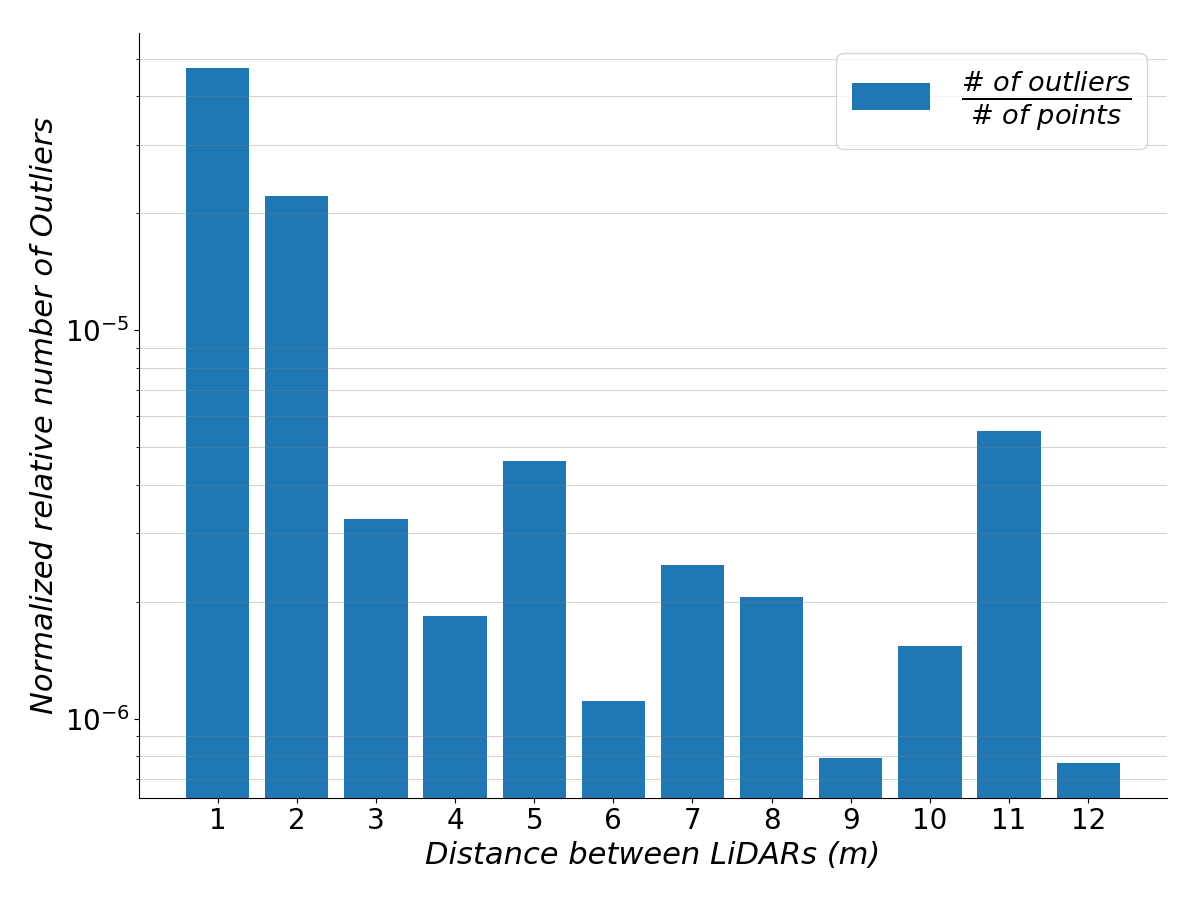
\includegraphics[width=0.8\textwidth]{img/lidar-interference/box-filtering/interference-box-filter-outliers-distance.png}
\caption[Relative number of outliers when the distance between the \acp{lidar} is varied on \ac{irislab}.]{Ratio between the number of outliers with respect to the total number of detected points accounting when the parameter under test is the distance between the two \acp{lidar}. The outlier accounting method is detailed in Equation~\eqref{eq:box-outlier-condition}.}
\label{fig:box-filter-outliers-distance}
\end{figure}

Despite the data not revealing any perceivable patterns, there is a tendency for the higher values of outliers to occur for a closer distance between the \acp{lidar}. Note that these results do not indicate that the interference is higher the shorter the distance, but that the interference causes a higher number of points to be outside of the room dimensions if the two \acp{lidar} are closer. 

\subsubsection{Height}
Due to the \ac{lidar} photodetectors and lasers orientation and internal organization, there are, theoretically, relative positioning and orientation between the two \acp{lidar} that either minimize the interference or potentiate it. No theoretical analysis of such relations was carried, due to its impracticality: the application of such results to an extent it would benefit this research, i.e., gathering data under positions of maximum and minimum interference, would require the alignment of a laser and a photodetector, whose position is only approximately known, in free space of two different rotating devices. To precisely known the distance and relative position of the optical components would require disassembling the \ac{lidar}, which is not an option.

For a fixed distance, our goal was to understand if variations of several orders of magnitude occurred when the relative height between the devices changed, which could hint on the relevance of the relative positioning between the \acp{lidar} and its impact on the \ac{lidar} interference behaviour.

Figure~\ref{fig:box-filter-outliers-height} shows our analyzes of this parameter by measuring the relative number of outliers outside the room dimensions. Height difference values, presented on the x-axis of the bar chart, indicate the relative height between the HESAI and the Velodyne \acp{lidar}. The interferer \ac{lidar} was placed at a distance of \SI{4}{\meter} of the victim and their relative orientation was kept approximately at \SI{0}{\degree}.

\begin{figure}[!ht]
\centering
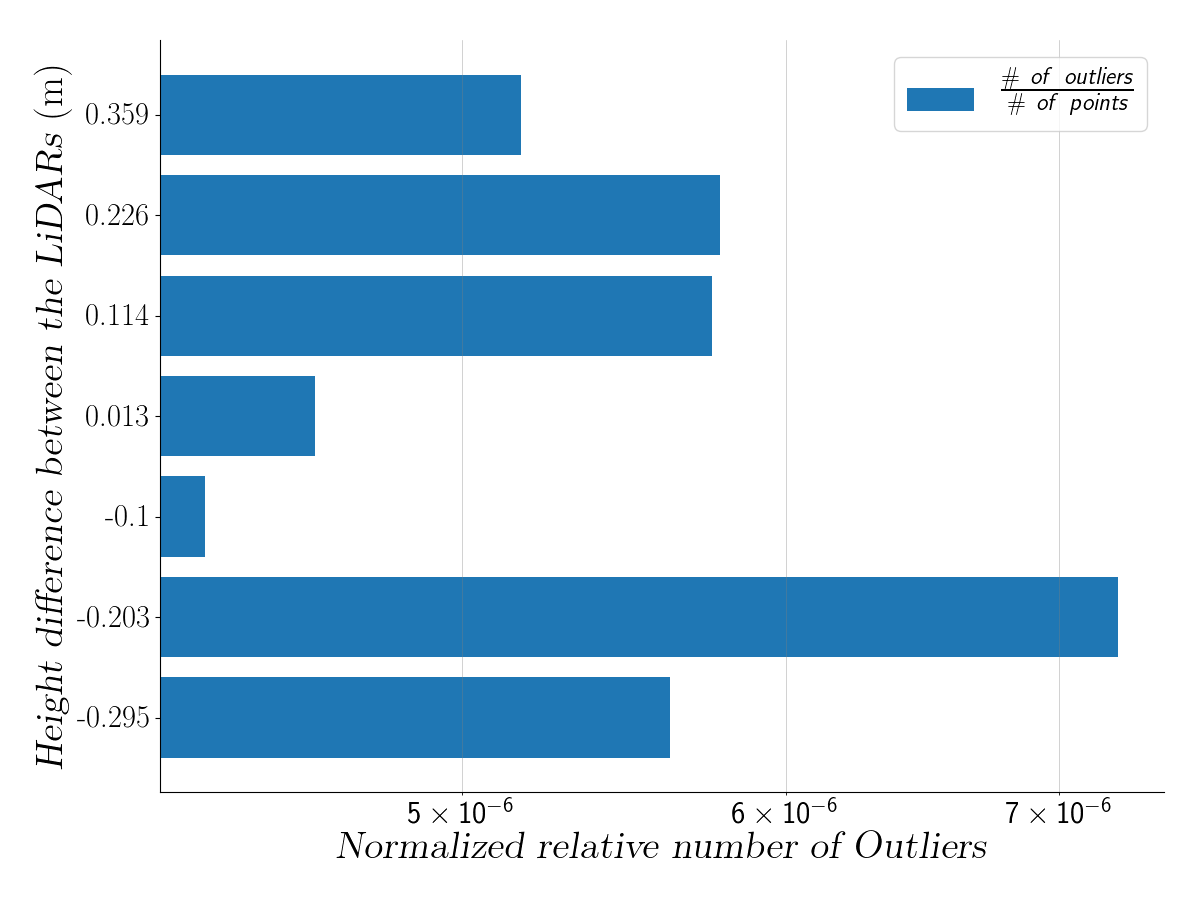
\includegraphics[width=0.8\textwidth]{img/lidar-interference/box-filtering/interference-box-filter-outliers-height.png}
\caption[Relative number of outliers when the height between the \acp{lidar} is varied on \ac{irislab}.]{Outliers analyzes when the parameter under test is height. On the x-axis, the height variation indicates the Pandar40 relative position in relation to the VLP-16 and is measured at their supposed optical centers.}
\label{fig:box-filter-outliers-height}
\end{figure}

The results obtained are all on the same order of magnitude, $10^{-6}$, having a variation, between its maximum and its minimum of approximately 7 times. They show that when their optical center is aligned, the number of outliers is at its lower, but coherent with the results of Figure~\ref{fig:box-filter-outliers-distance}: around $2\E^{-6}$. Despite the higher interference value occurring for a height difference of $\approx \SI{-0.2}{\meter}$, opting to place the interferer \ac{lidar} above or below the victim \ac{lidar} increases the number of outliers when comparing with the two \acp{lidar} being aligned. However, opting for above instead of below (or vice-versa) does not appear to have any significant advantage. 

\subsubsection{\acp{lidar} \ac{los} Obstruction}
To assess the impact of direct vs. indirect interference on the number of outliers, we obstructed the \acf{los} between the two \acp{lidar} with a straight box. The goal of this obstruction is to block direct beams between the two \acp{lidar}, therefore eliminating direct \ac{lidar} interference. With this contraption, data is recorded at even distances between the two \ac{lidar}, with the obstacle placed in their middle distance. As expected, when the distance is increased between the two \acp{lidar}, the distance between each of them to the obstacle also increases, resulting in a smaller angular occupation of the \acp{lidar} \ac{fov} with the obstacle. Reducing the angular occupation potentially increases the number of rays that can cause indirect interference on the victim's \ac{lidar}. However, no actions were taken to further investigate this premise.

In Figure~\ref{fig:box-filter-outliers-LOS}, the outlier analysis under a scenario of \ac{los} between the \acp{lidar} is shown. When comparing with the results of the distance test, Figure~\ref{fig:box-filter-outliers-distance}, a reduction of one order of magnitude is noticeable on all distances except at \SI{8}{\meter} and \SI{12}{\meter}, on which the number of outliers remain approximately equal. 

\begin{figure}[!ht]
\centering
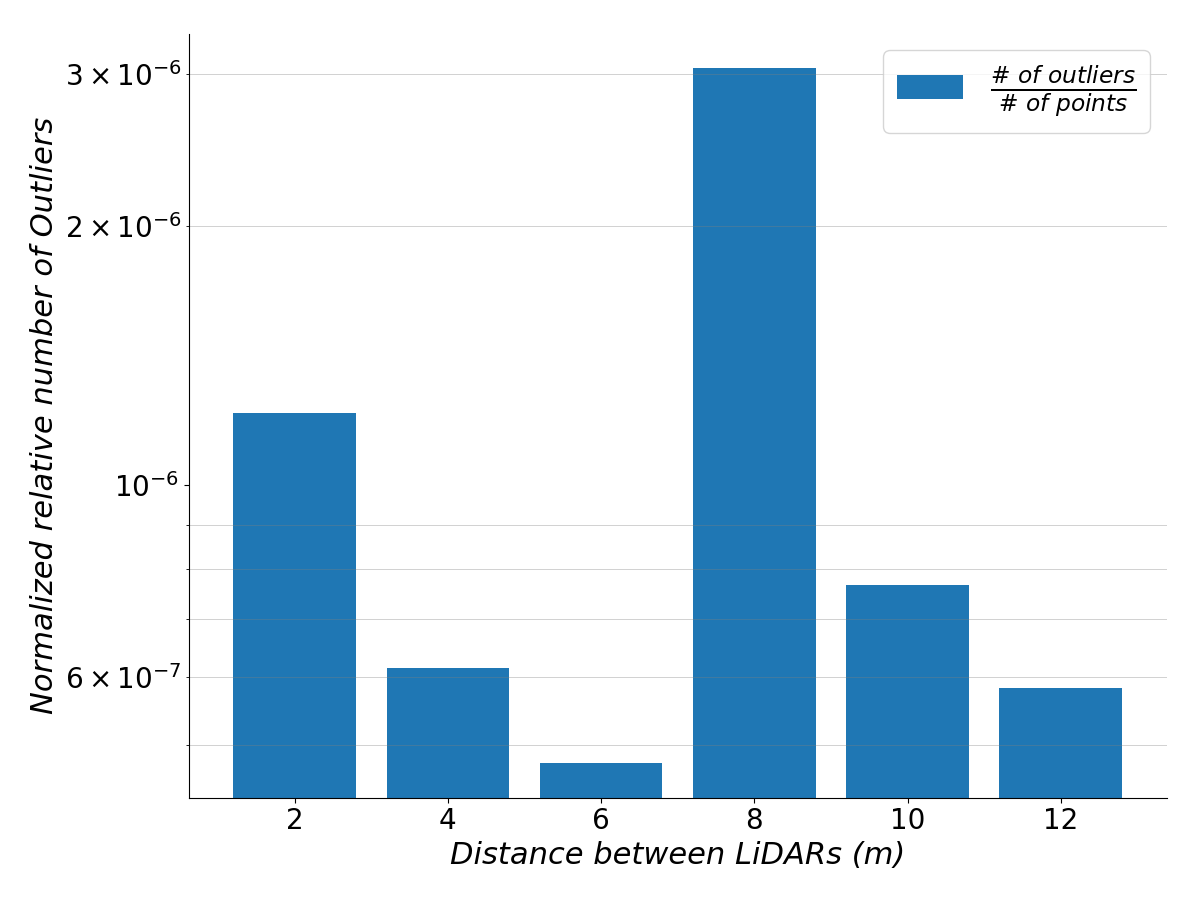
\includegraphics[width=0.8\textwidth]{img/lidar-interference/box-filtering/interference-box-filter-outliers-LOS.png}
\caption[Relative number of outliers when the \acp{lidar} \ac{los} is obstructed and the distance between the \acp{lidar} is varied, on \ac{irislab}.]{Relative number of outliers when the distance was varied, with an obstacle obstructing the \acp{lidar} \ac{los}. The distance variation correspond to the even numbers from the distance test and the obstacle was always placed in between the two \ac{lidar}.}
\label{fig:box-filter-outliers-LOS}
\end{figure}

Those findings make us believe that the most significant part of the outliers that are outside of the room are caused by direct interference. Two subsets of the graphics' data are monotonous descending: from \SIrange{2}{6}{\meter} and \SIrange{8}{12}{\meter}. Inside each of these subsets, the number of outliers reduces with the distance, but the behavior described on the distance test, were the major values of outliers occurred on short distances, is not verified here. We are also led to believe that at short distances, direct interference dominates, reason why on the distance setup without \ac{los} obstruction, the number of outliers is higher for short distances in comparison with \ac{los} obstruction.

\subsubsection{Relative orientation}
To comprehend whether the orientation between the \acp{lidar} affects the number of outliers, the interferer \ac{lidar} orientation was changed, keeping their relative distance constant. Tests were performed with an angular step of \SI{30}{\degree}, creating 12 data points that are shown in Figure~\ref{fig:box-filter-outliers-direction}.

\begin{figure}[!ht]
\centering
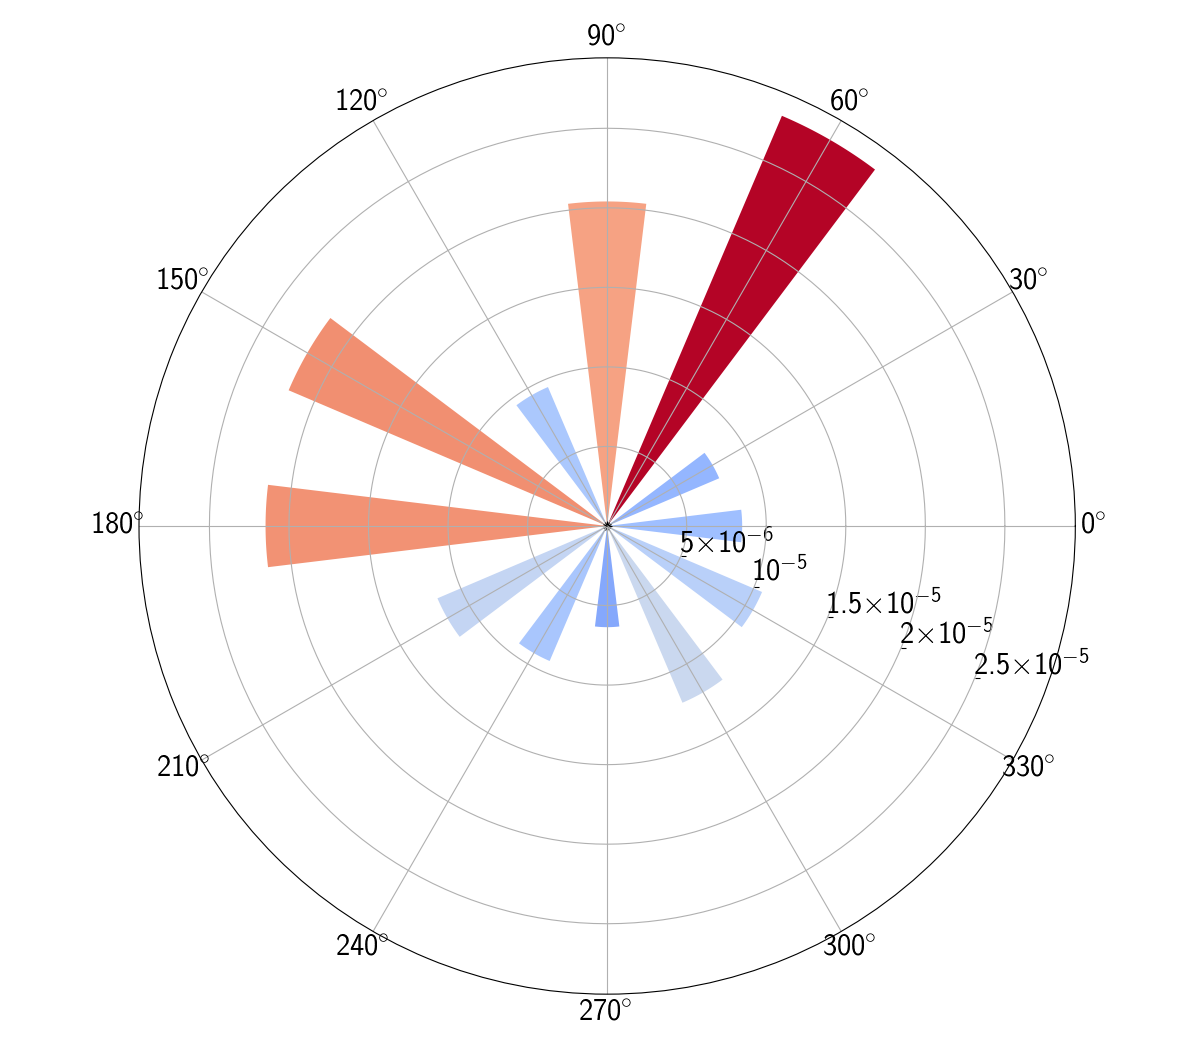
\includegraphics[width=0.8\textwidth]{img/lidar-interference/box-filtering/interference-box-filter-outliers-direction.png}
\caption[Relative number of outliers when the relative orientation between the \acp{lidar} is varied on \ac{irislab}.]{Normalized number of outliers, regarding the orientation between the \ac{lidar}. On this polar chart, the higher the bar, the higher the value of interference. For 4 angles (\SIlist[list-final-separator = {, }]{60; 90; 150; 180}{\degree}) the relative interference is ten times higher than the other angular positions.}
\label{fig:box-filter-outliers-direction}
\end{figure}

The normalized number of outliers magnitude variation between the angular positions results on a relative number of outliers to one in a million points or to one in ten million points. Some dependence with the relative \ac{lidar} orientation is present, with 4 angles, \SIlist[list-final-separator = {, }]{60; 90; 150; 180}{\degree}, having a normalized number of outliers one order of magnitude greater than the remaining 8 angles: $10^{-6}$ vs. $10^{-7}$.

We would expect that the angular position between \ac{tof} rotating \acp{lidar} with a \ac{fov} of \SI{360}{\degree} to not be dependent of the angular position in between the \acp{lidar}. Our results, however, show a preferred direction (\SI{60}{\degree}), but more tests are required to conclude about the impact of relative orientation. From these results, we also conclude that the \SI{30}{\degree} angular step was possible too high, since large variations between adjacent angular positions are registered.


% Note: Writing this here would imply creating figures that show the directionality of the data, i.e., play the rosbag files and accumulate them on Rviz. Alternatively, a point accumulator ros node ros node can be built ;)
%On Figure~\ref{fig:bosch-pandar-vs-vlp16}, we see a clearly directionality of data and from our findings, there seem to be a small impact of the orientation between \acp{lidar}. As we have stated, the scatter plot representation seems to empathize the problem of \ac{lidar} interference, making it seem more complex, when in reality, a heat map should be used instead to represent, in order to plot the density.


\subsubsection{\ac{it} Dark Room}
\ac{it} 2 Dark Room test methodology differs from the one used on \ac{irislab}, since two parameters were simultaneously varied, instead of only one: distance and height. The results presented in Figure~\ref{fig:box-filter-outliers-it2}. Along its x-axis, distance is varied and on its y-axis, the relative height between the \acp{lidar} is changed.

\begin{figure}[!ht]
\centering
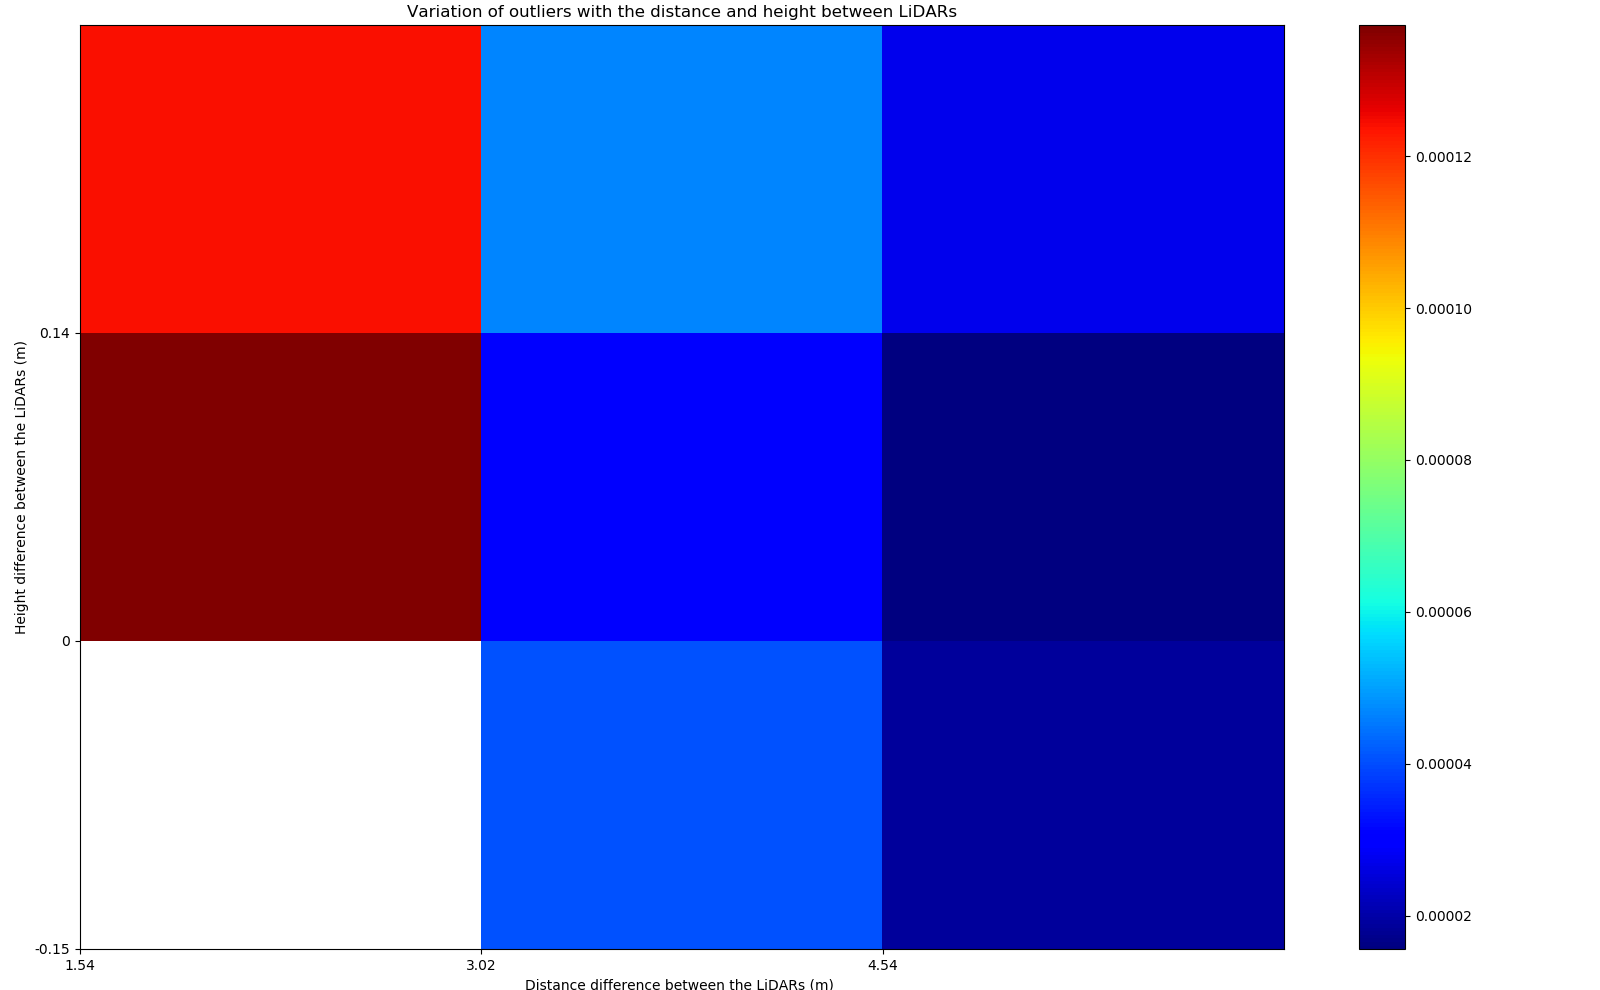
\includegraphics[width=0.8\textwidth]{img/lidar-interference/box-filtering/interference-box-filter-outliers-it2.png}
\caption[Relative number of outliers when the distance and height between the \acp{lidar} are varied on \ac{it} 2 Dark Room.]{\ac{it} 2 Dark Room results. Relative height and distance between the victim's and interferer \ac{lidar} were varied. Along the x-axis, distance variations between the \acp{lidar} are considered and on the y-axis, the height differences. The left bottom data point is blank due to data corruption.}
\label{fig:box-filter-outliers-it2}
\end{figure}

The white square on the left bottom of the figure is empty because the bag file containing that data was corrupted during saving and data could not be recovered. From the image, we corroborate the previous results from the distance tests (Figure~\ref{fig:box-filter-outliers-distance}): the closest the two \acp{lidar} are, the higher the number of outliers. If the interferer \ac{lidar} is above the victim's \ac{lidar}, the number of outliers also increases slightly, when comparing with the other heights tested, with the exception of the closest distance.



%%%%%%%%%%%%%%%%%%%%%%%%%%%%%%%%%%%%%%%%%%%%%%%%%%%%%%%%%%%%%%%%%%%%%%%%%%%%%%%%%%%%%%%%%%%%%%%%%
%%%%%%%%%%%%%%%%%%%%%%%%%%%%%%%%%% GROUND TRUTH GENERATION %%%%%%%%%%%%%%%%%%%%%%%%%%%%%%%%%%%%%%
%%%%%%%%%%%%%%%%%%%%%%%%%%%%%%%%%%%%%%%%%%%%%%%%%%%%%%%%%%%%%%%%%%%%%%%%%%%%%%%%%%%%%%%%%%%%%%%%%


\section{Ground-Truth Generation}
\label{sec:lidar-interference:ground-truth-generation}
To deepen our understanding of \ac{lidar} interference, the possibility that \ac{lidar} interference not only causes erroneous measures that are clearly outliers of the data, but also more subtle errors, possibly similar to sensor noise, must be considered. To test this premise, we need to compare the point clouds with interference with a known model of the environment, i.e., a ground-truth, that contains no interference.  

A ground truth model of the environment can be a specific point cloud from all the data or can be generated by considering multiple point cloud frames, from interference-free data. The latter is preferred, since it gives more chances of removing sensor noise from the data. Due to the lack of no viable alternatives on the \acl{sota}, we propose two algorithms for ground-truth generation, which are capable of fusing multiple point cloud frames from a bag file, generating a model that better resembles the real characteristics of the room.


\subsection{Frame Stitching}
\label{subsec:lidar-interference:frame-stitching}
Frame stitching consists of, given two point cloud frames, aligning a second point cloud frame with the first and then merge their data into a single point cloud frame. Iteratively performing this operation would create a single point cloud that progressively contains the best estimation of the environment point cloud, using multiple point clouds.

To implement this, first the two frames to be stitched are filtered, using \ac{pcl}'s Voxel Grid filter~\cite{PCL}, with a voxel edge length of \SI{5}{\centi\meter}. This step ensures the data density and spatial organization of the point clouds is similar, which yields better results on the stitching process and also speeds it up, due to a reduction of the data points.

To stitch the two voxelized data frames together, an \ac{icp} algorithm is used~\cite{Rusinkiewicz2001}. Our solution uses \ac{pcl} library and therefore, \ac{pcl}'s implementation of the \ac{icp} algorithm. \ac{icp} is an algorithm oriented to merge point clouds that have been acquired from different positions and only have some points in common. It performs the computation of the joint rotation and translation matrix, that transforms one point cloud coordinate frame to the others', aligning them. The computation of \ac{icp}'s transformation matrix uses \ac{svd} to compute the rotation and translation matrix that aligns the two point clouds~\cite{SVD, mvg_book}.

On our case, \ac{icp} will align the two point clouds, that are taken from the same position, but whose data, due to the \ac{lidar} measurement noise, will not be equal. The parameters used for this algorithm are presented in Table~\ref{tab:frame-stitching-parameters}. On \ac{icp}'s algorithm, the correspondences to be considered for the statistical analysis of the \ac{icp}'s convergence must be smaller than \SI{2}{\centi\meter}. Three termination criteria for the algorithm exist and must be tuned~\cite{PCL}:

\begin{enumerate}
\item \textbf{Maximum number of iterations:} If the algorithm reaches this number of interactions without converging, it stops and returns an error, indicating that it as not converged.
\item \textbf{Transformation Epsilon:} When iterating to refine the transformation computed internally, it terminates if the difference between the current and last transformation matrix is smaller than this parameter;
\item \textbf{Euclidean Difference Fitness Epsilon:} When iterating, terminates if the Euclidean errors (distance between the aligned source and target point cloud) is smaller than this threshold.
\end{enumerate}


\begin{table}[!ht]
\centering
\renewcommand{\arraystretch}{1.2}
\begin{tabular}{@{}lp{8cm}c@{}}
	\toprule
	\multicolumn{2}{l}{Specification} & Value \\
		\midrule
	\multicolumn{2}{l}{\textit{Voxel Filter}} & \\ 
	\phantom{ab} & Voxel edge length & \SI{5}{\centi\meter} \\ 
	\midrule
	\multicolumn{2}{l}{\textit{\ac{pcl}'s \ac{icp}}} &  \\ 
	\phantom{ab} & Maximum Correspondences Distance & \SI{2}{\centi\meter} \\
							 & Maximum Number of Iterations & 50 \\
							 & Transformation Epsilon & $1\E^{-8}$ \\
							 & Euclidean Difference Fitness Epsilon & \SI{5}{\centi\meter} \\
	\bottomrule
\end{tabular}
\caption[Parameters used on the Frame Stitching algorithm, for the ground-truth model generation.]{Parameter values used on the Frame Stitching algorithm, for the Voxel Grid and \ac{icp}.}
\label{tab:frame-stitching-parameters}
\end{table}

When it finishes computing the ground truth point cloud, the \ac{ros} node that implements this algorithm saves the ground truth \ac{lidar} point cloud on a \ac{pcd} file, the standard extension to save point cloud data on \ac{pcl}~\cite{PCL}.

This solution has some caveats, since it considers one of the point cloud frames to be the source to which all the other frames must be matched, i.e, the second frame is stitched to match the first frame, and the third frame is stitched to match the result of the second and first frame. The process is repeated iteratively until no frames remain. Also, despite \ac{pcl} being a templated library that can work with whatever point types are defined by the user, \ac{pcl} \ac{icp} implementation destroys the laser ID information that point clouds obtained from the VLP-16 contain, which limits the possibilities for posterior interference analysis. 


\subsection{Frame Registration}
\label{subsec:lidar-interference:frame-registration}
Frame Registration is a proposed ground truth model generation algorithm based on an organized point cloud data structure, which was primarily developed for \ac{lidar} interference analysis, but was later generalized to be used for ground truth model generation.

An organized point cloud is a data structure similar to the point cloud previously used, but its two-dimensional organization contains information about the adjacent points of a given point. This spacial organization mimics a depth image, with rows and columns, but differs from the latter since the data containing on each index of the data matrix is not only depth, but instead a point cloud point.

Our implementation, which extends \ac{pcl}'s organized point data structure, is a generic and templated data structure, that can support not only point cloud points as its basis data type. This peculiarity allows the usage of abstract point cloud containers, which contain point cloud data, but also other metrics, for every index of the data matrix. For ground truth generation, the container developed holds a vector of point cloud points, to store the registered point cloud points for that index. Fields for the intensity, position and distance are also available, both for the average value and the variance.

The developed ground truth technique computes, for every point of all the point cloud frames on a bag file, the index (row and column) to which that point belongs on the organized point cloud structure, and appends it to the point vector of that index container. On spherical coordinates, the point row index corresponds to its azimuthal angle and the column to its polar angle. On Velodyne \ac{lidar}'s, the polar angle is determined by the laser ID from which the pulse was fired and the azimuthal angle can be determined by Equation~\eqref{eq:azimuthal-angle}, from which the $x$ and $y$ coordinates are known from the point data. From the azimuthal angle, the azimuthal index of the matrix can be found by dividing the azimuthal angle with the angular step of the VLP-16, as shown in Equation~\eqref{eq:azimuthal-angle-index}.

\begin{equation}
\label{eq:azimuthal-angle}
\theta = \arctan\left(\frac{y}{x}\right) \cdot \frac{\SI{180}{\degree}}{\pi}
\end{equation}

\begin{equation}
\label{eq:azimuthal-angle-index}
\theta_{\text{index}} = \frac{\theta}{\text{VLP-16 angular step}} = \frac{\theta}{\SI{0.2}{\degree}} 
\end{equation}


After registering the full point cloud data, the ground truth model can be generated. Our implementation uses an average estimator that iterates over all the indexes of the matrix, computing the average point cloud coordinate using the vector of points registered, which will be the ground truth model coordinates. Alongside this position value for the ground truth model, this estimator also computes the variance and average value of the point of vectors distance and intensity.



%\subsection{Comparison}

%Direct interference (on Kim's experimental setup and hardware) is likely to saturate the receptor of the interfered \ac{lidar}, which may or may not be considered a valid measurement by the hardware and may discarded by the driver before being registered;


%%%%%%%%%%%%%%%%%%%%%%%%%%%%%%%%%%%%%%%%%%%%%%%%%%%%%%%%%%%%%%%%%%%%%%%%%%%%%%%%%%%%%%%%%%%%%%%%%
%%%%%%%%%%%%%%%%%%%%%%%%%%%%%%%%%% VOXEL TO VOXEL ANALYSIS %%%%%%%%%%%%%%%%%%%%%%%%%%%%%%%%%%%%%%
%%%%%%%%%%%%%%%%%%%%%%%%%%%%%%%%%%%%%%%%%%%%%%%%%%%%%%%%%%%%%%%%%%%%%%%%%%%%%%%%%%%%%%%%%%%%%%%%%

\section{Voxel-to-Voxel Analysis}
\label{sec:lidar-interference:voxel-analysis}
Voxel-to-voxel analysis quantifies the magnitude of the \ac{lidar} interference by measuring the amount of modified voxels between two tridimensional voxel grids: one that represents the ground truth model and another for each frame of the interference bag file.

Voxel Grids convey spatial representation of tridimensional data in a cluster of adjacent ``cubes'', each with the same edge length. Understanding which voxels have been modified in the point cloud means comparing, voxel by voxel, the state of occupation of the voxels in the ground truth voxel grid with the corresponding voxel on the interfered data voxel grid. 

On the \ac{lidar} interference scenario, since the scenario is static, an interference is said to have occurred in a voxel if its value between the ground-truth model and interfered point cloud frame is different, i.e., if it was occupied in the ground truth model and is free on the interference point cloud frame or was free on the ground truth model and is occupied in the interference point cloud frame. This condition can be expressed as a boolean XOR operation between the two voxels to be compared (Equation~\eqref{eq:voxel-interference-condition}), where a result of \texttt{1} represents a voxel whose state has changed (therefore, was interfered) and a result of \texttt{0} a voxel whose state remained constant (therefore, without interference).

\begin{equation}
	\label{eq:voxel-interference-condition}
	\text{Voxel has interference} = \text{Voxel}_\text{ground\_truth} \oplus  \text{Voxel}_\text{interference} 
\end{equation}

The relative number of modified voxels can be obtained by the summation of Equation~\eqref{eq:voxel-interference-condition}, for all the voxels that are present on the voxel grid. Equation~\eqref{eq:normalized-interference-voxels} describes this operation, where $N_x$, $N_y$ and $N_z$ are the number of voxels along each of its subscript dimensions, that can be computed by Equation~\eqref{eq:voxel-grid-limits}.

\begin{equation}
\label{eq:normalized-interference-voxels}
\text{Normalized Interfered Voxels} =\displaystyle \frac{\sum\limits^{N_x - 1}_{i = 0} \sum\limits^{N_y - 1}_{j = 0} \sum\limits^{N_z - 1}_{k = 0} \text{Voxel}_\text{ground\_truth}^{ijk} \oplus  \text{Voxel}_\text{interference}^{ijk}}{N_x\cdot N_y\cdot N_z}
\end{equation}

\begin{equation}
\label{eq:voxel-grid-limits}
N_i = \frac{\max(i) - \min(i)}{\text{Voxel edge length}}, \qquad \forall i \in \{x, y, z\}.
\end{equation}

\subsection{Implementation}
Voxelizing\footnote{Voxelizing: converting a point cloud representation using points to one using voxels.} the \ac{lidar} data would require, for the interference bag file, a voxel grid of \SI{260}{\meter} for each axis, since the \ac{lidar} drivers reject distance measurements beyond \SI{130}{\meter}. If a voxel grid with \SI{1}{\centi\meter} of edge length is used, such grid would have almost 1.76 billion voxels for a single point cloud frame. Assuming the simplest of scenarios, when each point is represented by 3 floating-point number of single precision, we would require $3\times \SI{4}{\bytes} = \SI{12}{\bytes}$ per point, yielding more than \SI{60}{\giga\byte} of data to manipulate and store. Most of it, however, would correspond to empty voxels.

Our solution consists on replacing the full tridimensional voxel grid with a data structure that has the same structure, but is more efficient: an octree. An octree is a tree-like data structure used to partition three-dimensional space, where every node has 8 children, each corresponding to one of the 8 octants of a tridimensional Cartesian coordinate frame, recursively diving the tridimensional space. This solution is effective because, similarly to a binary tree in 1D space, it only subdivides the 3D space if it requires more detail to represent a data point, therefore efficient being in memory occupation.

Out implementation relies on \ac{pcl}'s Octree Structure. In particular, \texttt{OctreePointCloudChangeDetector} class is used, which is built to detect changes on the octree structure when comparing the voxel representation of two point clouds: a ground truth model and each interference point cloud frame. 

Using the pre-determined ground truth models (see Section~\ref{sec:lidar-interference:ground-truth-generation}), an octree representation of the ground truth model is used as the source with which all the other point clouds will be compared. Then, frame by frame, the interferer bag file point clouds are loaded, converted to their octree representation, and then both octree representations are compared. The voxels which have changed from one octree to the other are accounted, considering all the frames of the bag file, using Equation~\eqref{eq:normalized-interference-voxels}.


\subsection{Results}
\label{subsec:lidar-interference:voxel-to-voxel-analysis}

To test this method of analysis, some parameters under test were selected from the dataset:relative distance between the two \acp{lidar}; relative height between the two \acp{lidar}; and the relative distance between the two \acp{lidar} under \ac{los} obstruction. The voxel edge length was also varied in steps of \SI{0.05}{\meter}, from \SIrange{0.05}{0.45}{\meter}.

Voxel-to-Voxel analysis has a caveat that must be considered: increasing the voxel edge size reduces the number of voxels that exist on the octree. Also, since octree's represent tridimensional data, doubling the voxel edge length could result on a reduction of the octree voxels number up to an eighth of the previous number of voxels. 

Large numbers of voxels (small voxel edge length) potentiates the occurrence of false positives\footnote{Voxels that are erroneously marked as interfered, because their state of occupancy was modified.}, because noisy points can alternate between two adjacent voxels. Fewer voxels (large voxel edge length), results in an increase of false negatives\footnote{Interfered voxels that are erroneously marked as non-interfered, because their state of occupancy was not modified.}, because measurements whose interference modified their positioning by a small error still belong to the same voxel. False positives are problematic because they indicate that the interference value is higher than really is and in contrast, false negatives reveal an interference value that is lower than the real value of interference.

Our particular implementation has yet another issue. Since the relative number of modified voxels is expressed relatively to the total number of voxels, changing the voxel edge length also changes the total number of voxels, which in turn changes the relative number of modified voxels. For a large voxel edge length, this behavior might cause the interference to actually be higher than the real value, due to the number of voxels being smaller. 

To minimize the undesired impact of this behavior, we choose a voxel edge interval between \SI{0.05}{\meter} and \SI{0.45}{\meter}. The first boundary is determined by the typical \ac{lidar} accuracy value, $\pm\SI{3}{\centi\meter}$~\cite{VLP16}. The second is determined by analyzing our dataset, which on average has a reduction of 4 times the number of voxels when the voxel edge length is doubled. Our objects of interest on the dataset (chairs, person dummies, boxes, among others) have a size ranging from \SIrange{0.3}{1.1}{\meter}, approximately. 

To keep the voxel edge length small, we opt to choose a voxel edge length below a meter. Following this premise, the difference between a voxel edge length of \SI{0.40}{\meter} and \SI{0.80}{\meter} is an increase of 8 times in volume of the voxel. This difference, at the dimensions being discussed, is sufficient to contain noisy data from the measurements, reducing false positives, but also to generate some false negatives. Therefore, we choose the lower value for the voxel edge length, \SI{0.40}{\meter} and compute all the results for the voxel length following it, \SI{0.45}{\meter}.

To understand the behavior of our ground truth generation algorithm, we opt also to analyze the relative number of modified voxels between the ground truth model and the ground truth point clouds used to generate it. To assess the difference between the results, these are also subtracted, to compare their relative number of voxels modified by the ground-truth bag file and the interference bag file. The ground-truth model generation method used on the Voxel-to-Voxel analysis is Frame Stitching, detailed in sub-Section~\ref{subsec:lidar-interference:frame-stitching}.

\subsubsection{Distance}
For all the distance values (\SIrange{1}{12}{\meter} with a step of \SI{1}{\meter}), the voxel edge length was varied from \SIrange{0.05}{0.45}{\meter}, with steps of \SI{0.05}{\meter}. The comparison between the ground truth model and the interference bag are shown in sub-Figure~\ref{fig:distance:octree-interference-color-mesh} and the results of repeating the analysis between the ground truth model and the ground truth bag file used to generate it are shown in Figure~\ref{fig:distance:octree-ground-truth-color-mesh}. 

\begin{figure}[!ht]
\centering
\begin{subfigure}[c]{0.45\textwidth}
	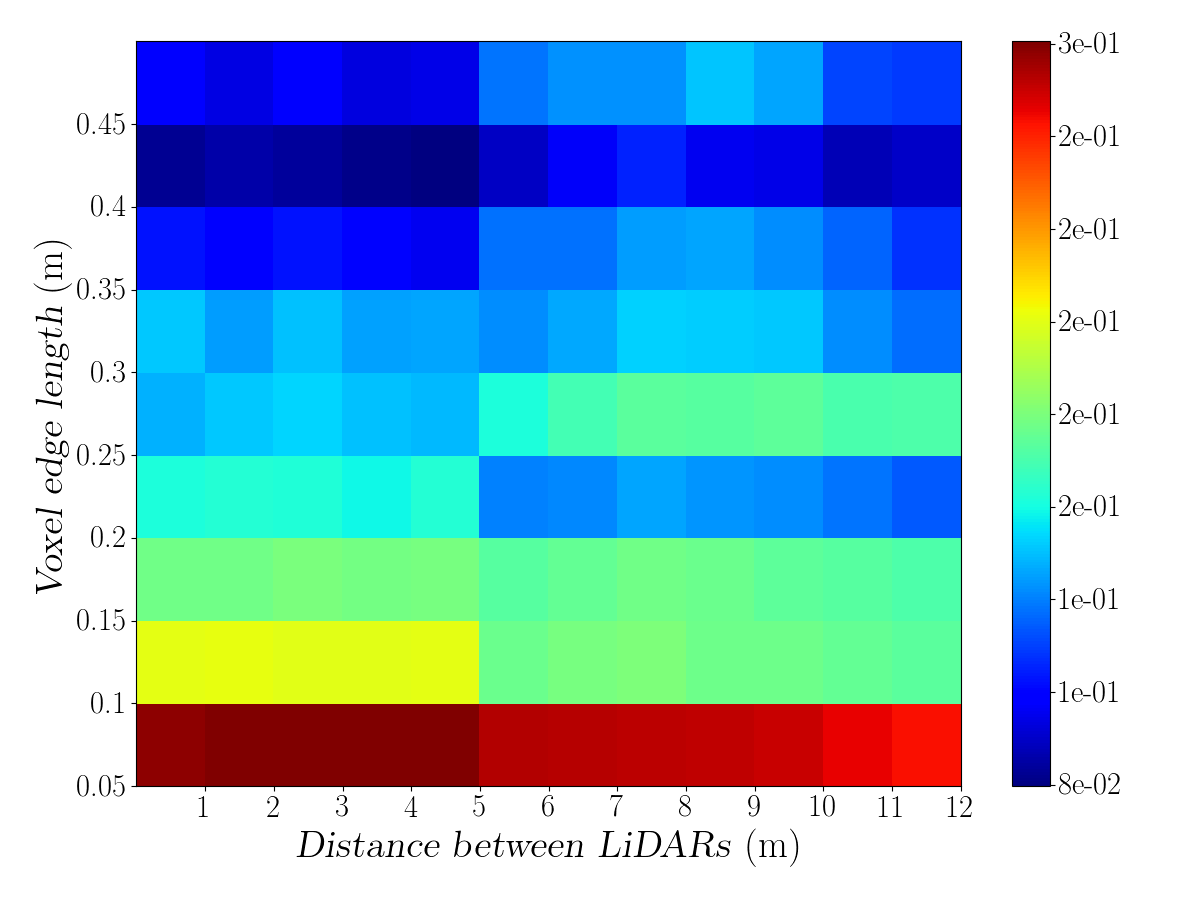
\includegraphics[width=\textwidth]{img/lidar-interference/distance/octree_interference_color_mesh.png}
\caption{}%Voxel-to-Voxel analysis results when comparing the interference bag file with the ground truth model.}
	\label{fig:distance:octree-interference-color-mesh}
\end{subfigure}
\qquad
\begin{subfigure}[c]{0.45\textwidth}
	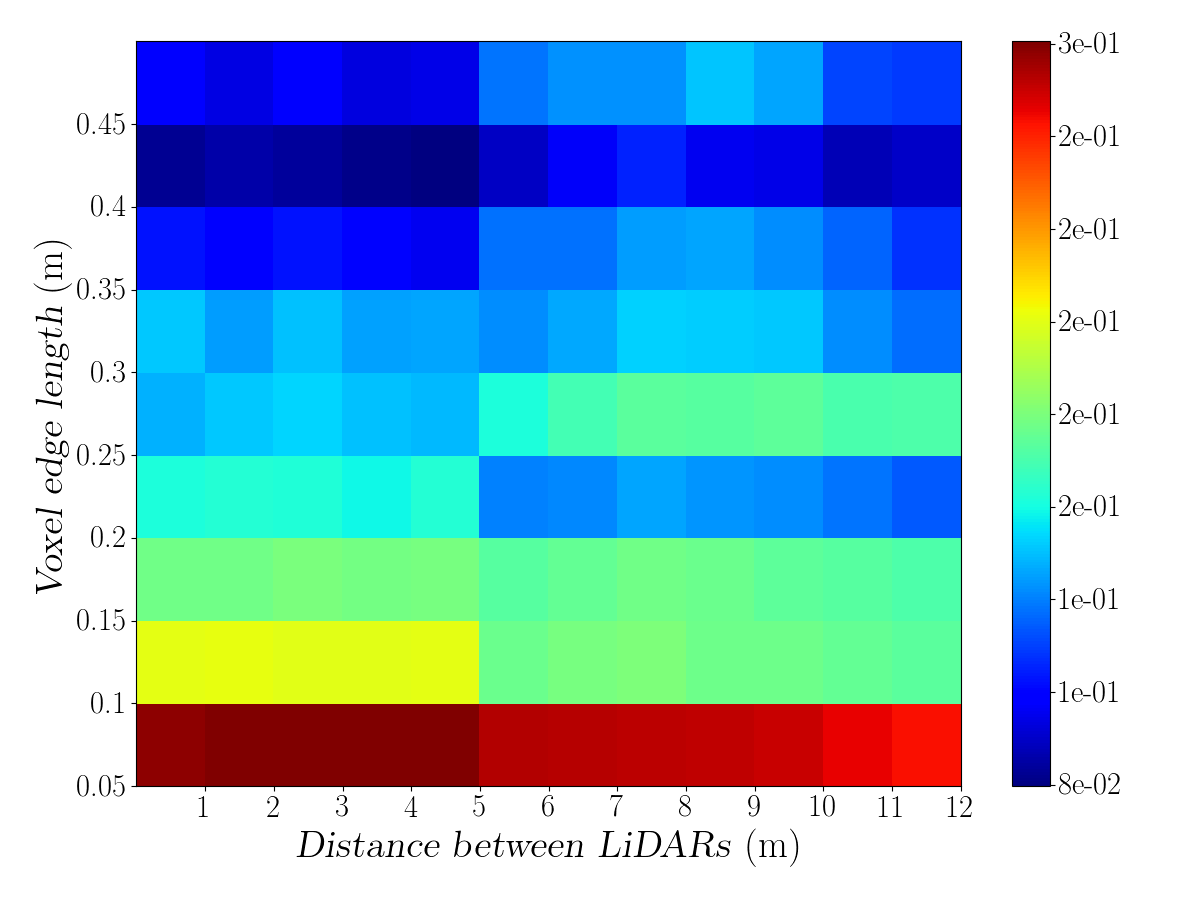
\includegraphics[width=\textwidth]{img/lidar-interference/distance/octree_ground_truth_color_mesh.png}
\caption{}%Voxel-to-Voxel analysis results when comparing the ground truth bag file with the ground truth model.}
	\label{fig:distance:octree-ground-truth-color-mesh}
\end{subfigure}
\\ \vspace{4mm}
\begin{subfigure}[c]{0.6\textwidth}
	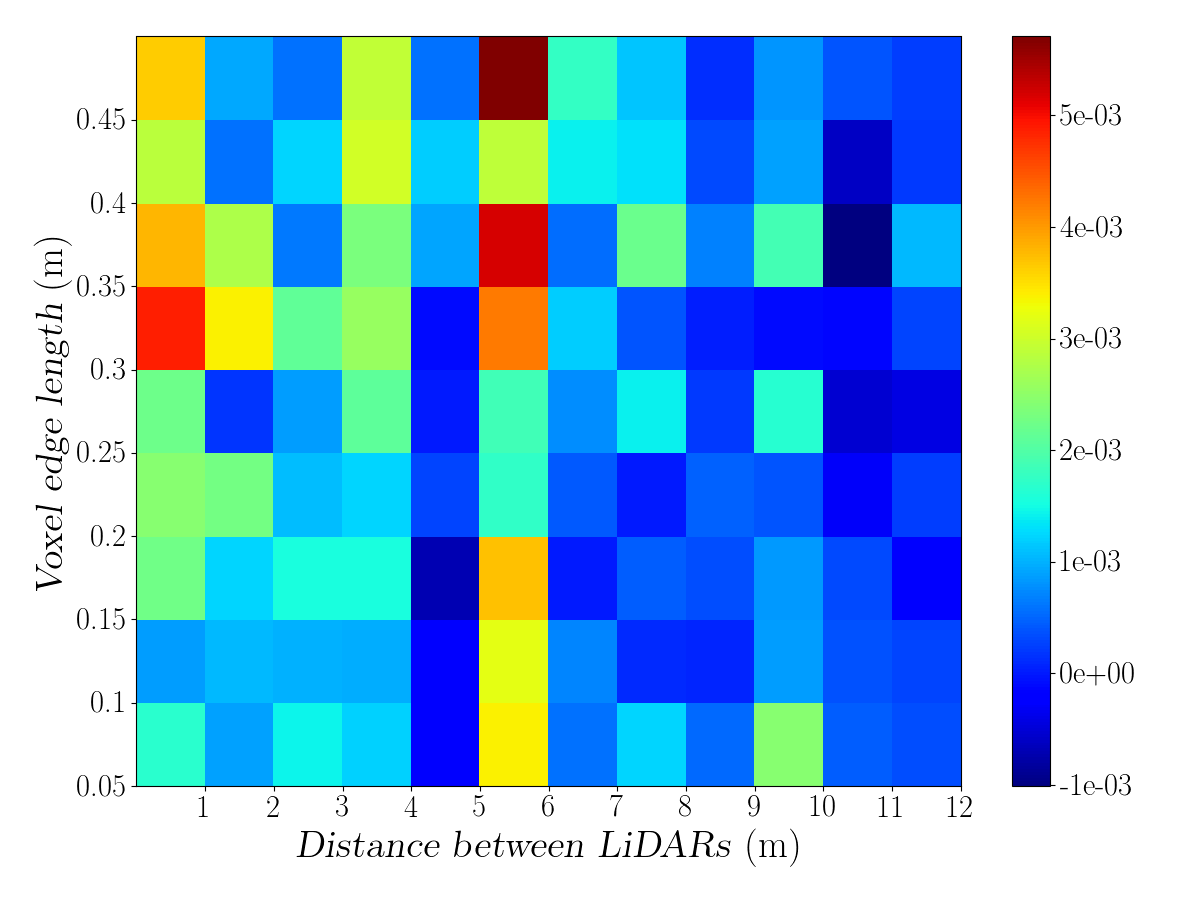
\includegraphics[width=\textwidth]{img/lidar-interference/distance/octree_difference_color_mesh.png}
	\caption{}%Voxel-to-Voxel analysis results when computing the difference between the results on sub-Figure~(\subref{fig:distance:octree-interference-color-mesh}) and sub-Figure~(\subref{fig:distance:octree-ground-truth-color-mesh}).}
	\label{fig:distance:octree-difference-color-mesh}
\end{subfigure}

\caption[Voxel-to-Voxel analysis when the distance between the \acp{lidar} is variated.]{Voxel-to-Voxel \ac{lidar} interference analysis when the parameter under test is the relative distance between the two \acp{lidar}, victim and interferer. In sub-Figure~(\subref{fig:distance:octree-interference-color-mesh}), the interfered bag is compared against the ground truth model and in sub-Figure~(\subref{fig:distance:octree-ground-truth-color-mesh}), the ground truth bag file is compared with the ground truth model. The latter results are subtracted to the former, resulting in sub-Figure~(\subref{fig:distance:octree-difference-color-mesh}). For every sub-figure, the x-axis shows the distance between the \acp{lidar} and the y-axis the different values of voxel edge length to which tests were made.}
\label{fig:distance:octree-color-mesh}
\end{figure}

Analyzing sub-Figure~\ref{fig:distance:octree-interference-color-mesh}, the relative number of modified voxels is 27.5\%, meaning that for a voxel grid size of $\SI{5}{\centi\meter}\times \SI{5}{\centi\meter}\times \SI{5}{\centi\meter}$, 27.5\% of the voxels which contain data were changed. Sub-Figure~\ref{fig:distance:octree-ground-truth-color-mesh}, which compares the ground-truth model with the ground-truth bag file, shows similar results.  

Despite a small variation of the relative number of modified voxel with the parameter under test (on the x-axis), the rate of change is greater on the y-axis with the increase of the voxel edge length. After a voxel edge length of \SI{0.3}{\meter}, the relative number of interfered voxels tends to stabilize. 

The subtraction between the relative number of modified voxels on the interference and ground truth bags is given in sub-Figure~\ref{fig:distance:octree-difference-color-mesh}. On this image, in general, the number is positive, which means that due to interference, the number of changes on the interference bag are greater than on the ground truth bag. The order of magnitude of the number of modified voxels between the two datasets is $10^{-3}$, which indicates that, on average one in each thousand voxels has changed its occupation status, due to its points being interfered and wrongly measured.


\subsubsection{Height}
For all the relative height values between the two \acp{lidar} (\SIlist[list-units=single]{0.623; 0.715; 0.818; 0.931; 1.032; 1.144; 1.277}{\meter}), the voxel edge length value was varied from \SIrange{0.05}{0.45}{\meter}, with steps of \SI{0.05}{\meter}. The comparison between the ground truth model and the interference bag is shown in sub-Figure~\ref{fig:height:octree-interference-color-mesh} and the results of repeating the analysis between the ground truth model and the ground truth bag file used to generate it are shown in Figure~\ref{fig:height:octree-ground-truth-color-mesh}.

\begin{figure}[!ht]
\centering
\begin{subfigure}[c]{0.45\textwidth}
	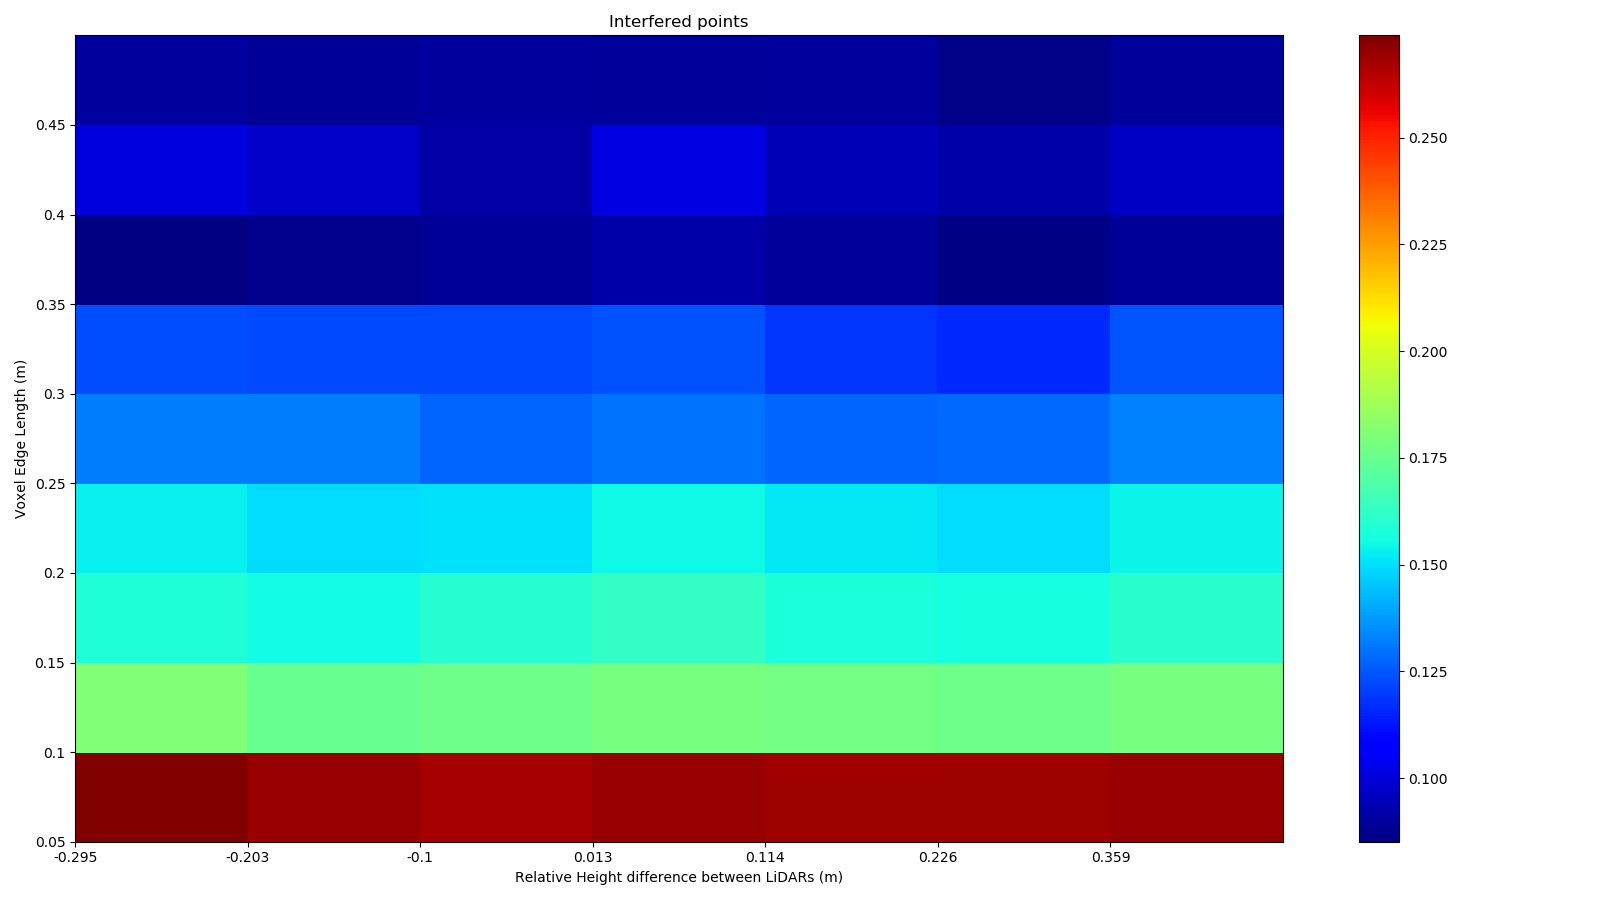
\includegraphics[width=\textwidth]{img/lidar-interference/height/octree_interference_color_mesh.png}
\caption{}%Voxel-to-Voxel analysis results when comparing the interference bag file with the ground truth model.}
	\label{fig:height:octree-interference-color-mesh}
\end{subfigure}
\qquad
\begin{subfigure}[c]{0.45\textwidth}
	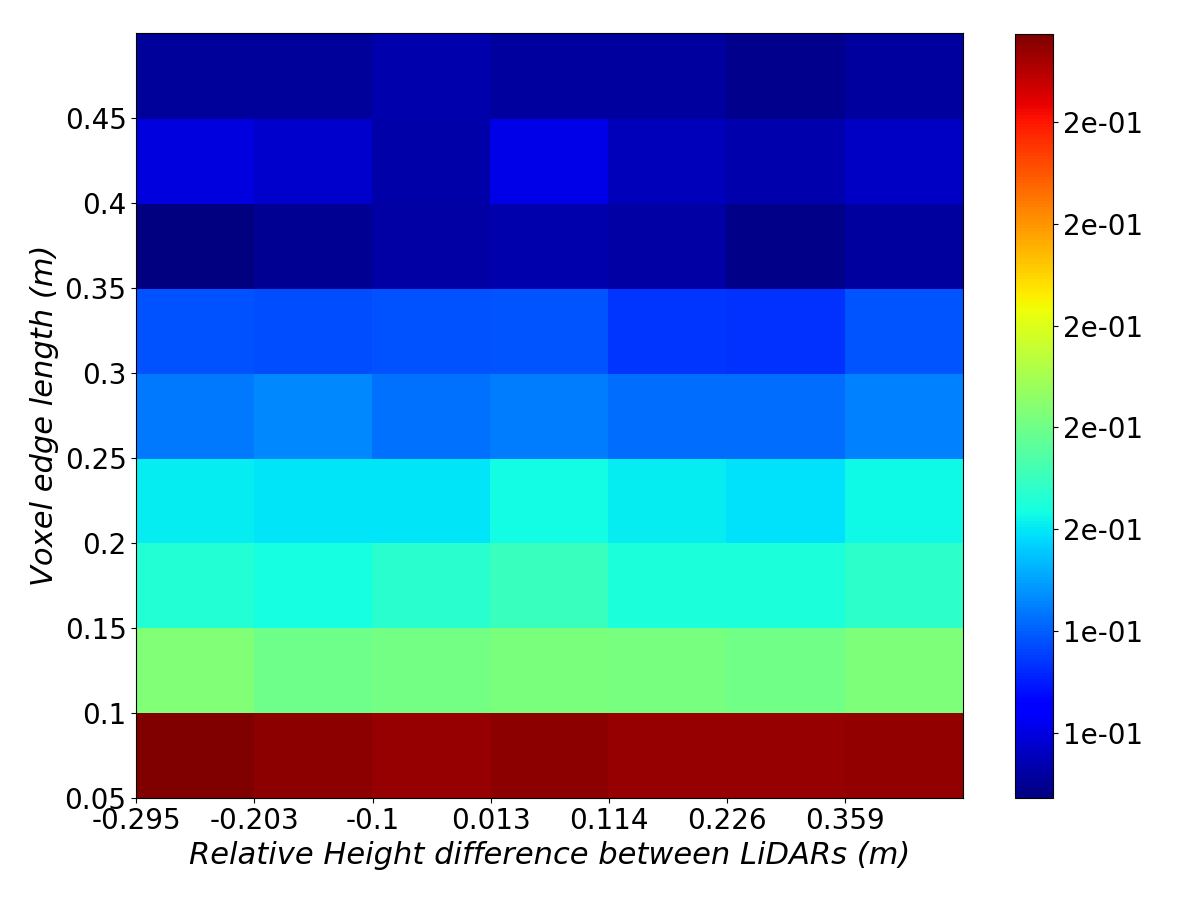
\includegraphics[width=\textwidth]{img/lidar-interference/height/octree_ground_truth_color_mesh.png}
\caption{}%Voxel-to-Voxel analysis results when comparing the ground truth bag file with the ground truth model.}
	\label{fig:height:octree-ground-truth-color-mesh}
\end{subfigure}
\\ \vspace{4mm}
\begin{subfigure}[c]{0.6\textwidth}
	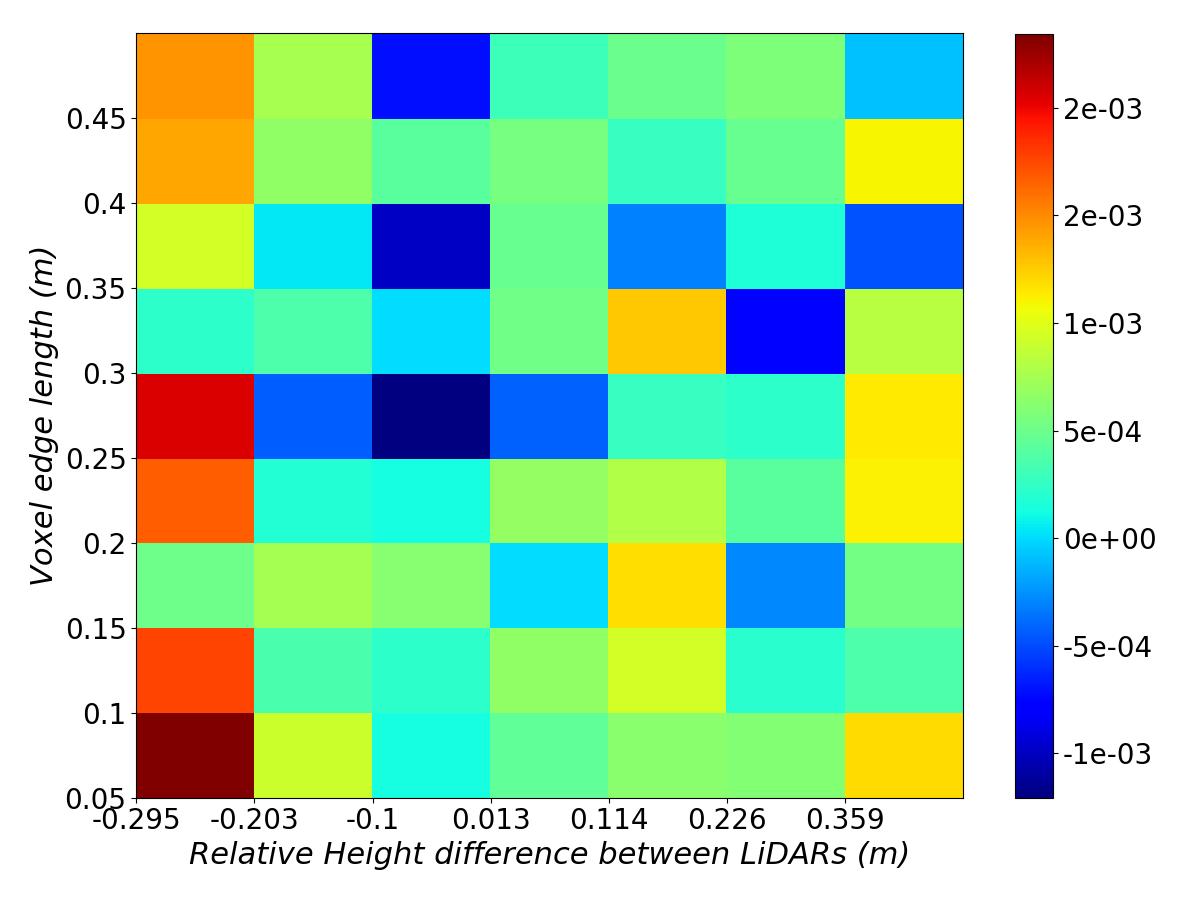
\includegraphics[width=\textwidth]{img/lidar-interference/height/octree_difference_color_mesh.png}
\caption{}%Voxel-to-Voxel analysis results when computing the difference between the results on sub-Figure~(\subref{fig:height:octree-interference-color-mesh}) and sub-Figure~(\subref{fig:height:octree-ground-truth-color-mesh}).}
	\label{fig:height:octree-difference-color-mesh}
\end{subfigure}

\caption[Voxel-to-Voxel analysis when the height between the \acp{lidar} is variated.]{Voxel-to-Voxel \ac{lidar} interference analysis when the parameter under test is the relative distance between the two \acp{lidar}, victim and interferer. In sub-Figure~(\subref{fig:height:octree-interference-color-mesh}), the interfered bag is compared against the ground truth model and in sub-Figure~(\subref{fig:height:octree-ground-truth-color-mesh}), the ground truth bag file is compared with the ground truth model. The latter results are subtracted to the former, resulting in sub-Figure~(\subref{fig:height:octree-difference-color-mesh}). For every sub-figure, the x-axis shows the relative height between the \acp{lidar} optical center and the y-axis the different values of voxel edge length to which tests were made.}
\label{fig:height:octree-color-mesh}
\end{figure}

Analyzing sub-Figure~\ref{fig:height:octree-interference-color-mesh}, the relative number of modified voxels is 25.0\%, meaning that for a voxel grid size of $\SI{5}{\centi\meter}\times \SI{5}{\centi\meter}\times \SI{5}{\centi\meter}$, 25.0\% of the voxels which contain data were changed. However, comparing this results with the equivalent sub-figure, but which compares the ground-truth model with the ground-truth bag file, sub-Figure~\ref{fig:distance:octree-ground-truth-color-mesh}, shows similar results.

Despite a small variation of the relative number of modified voxels with the parameter under test (on the x-axis), the rate of change is greater on the y-axis with the increase of the voxel edge length. After a voxel edge length of \SI{0.25}{\meter}, the relative number of interfered voxels tends to stabilize. 

The subtraction between the relative number of modified voxels on the interference and ground truth bags is shown in sub-Figure~\ref{fig:height:octree-difference-color-mesh}. On this image, in general, the subtraction yields positive results, which implies that due to interference, the number of changes on the interference bag are greater than on the ground truth bag. The order of magnitude of the number of modified voxels between the two datasets ranges from $10^{-4}$ to $10^{-3}$, which indicates that, on average one in each thousand voxels has changed its occupation status, due to its points being interfered and wrongly measured.


\subsubsection{\acp{lidar} \ac{los} Obstruction}
For all the distance values that the \acf{los} between the two \acp{lidar} was obstructed (\SIrange{1}{12}{\meter} with a step of \SI{2}{\meter}), the voxel edge length was varied from \SIrange{0.05}{0.45}{\meter}, with steps of \SI{0.05}{\meter}. The comparison between the ground truth model and the interference bag are shown in sub-Figure~\ref{fig:los:octree-interference-color-mesh} and the results of repeating the analysis between the ground truth model and the ground truth bag file used to generate it are shown in Figure~\ref{fig:los:octree-ground-truth-color-mesh}.

\begin{figure}[!ht]
\centering
\begin{subfigure}[c]{0.45\textwidth}
	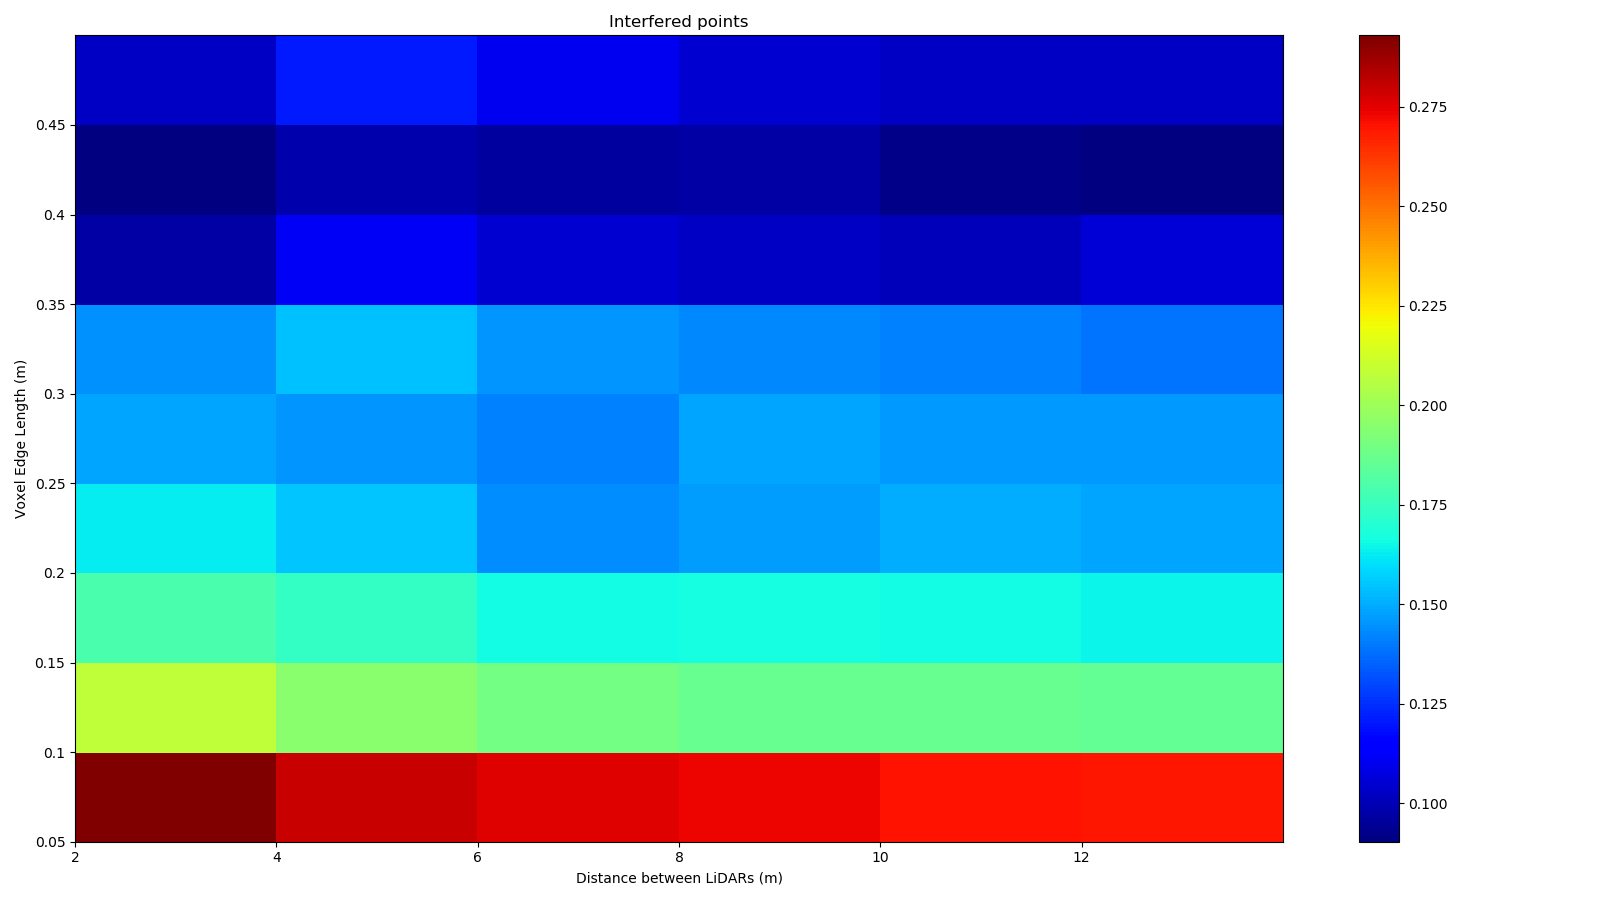
\includegraphics[width=\textwidth]{img/lidar-interference/LOS/octree_interference_color_mesh.png}
	\caption{}%Voxel-to-Voxel analysis results when comparing the interference bag file with the ground truth model.}
	\label{fig:los:octree-interference-color-mesh}
\end{subfigure}
\qquad
\begin{subfigure}[c]{0.45\textwidth}
	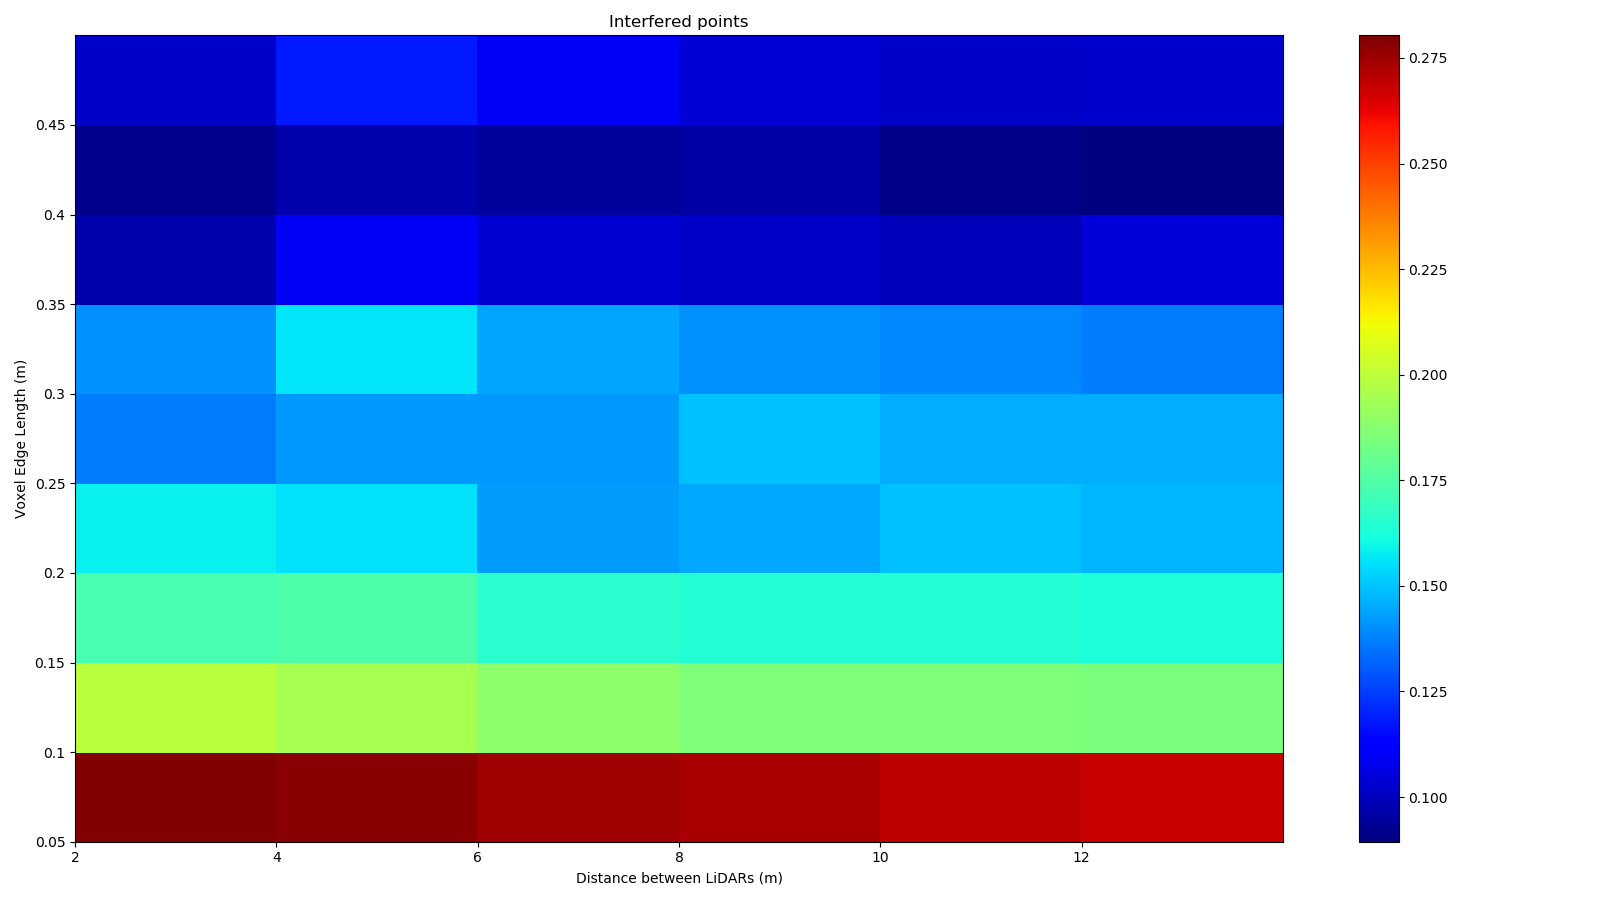
\includegraphics[width=\textwidth]{img/lidar-interference/LOS/octree_ground_truth_color_mesh.png}
\caption{}%Voxel-to-Voxel analysis results when comparing the ground truth bag file with the ground truth model.}
	\label{fig:los:octree-ground-truth-color-mesh}
\end{subfigure}
\\ \vspace{4mm}
\begin{subfigure}[c]{0.6\textwidth}
	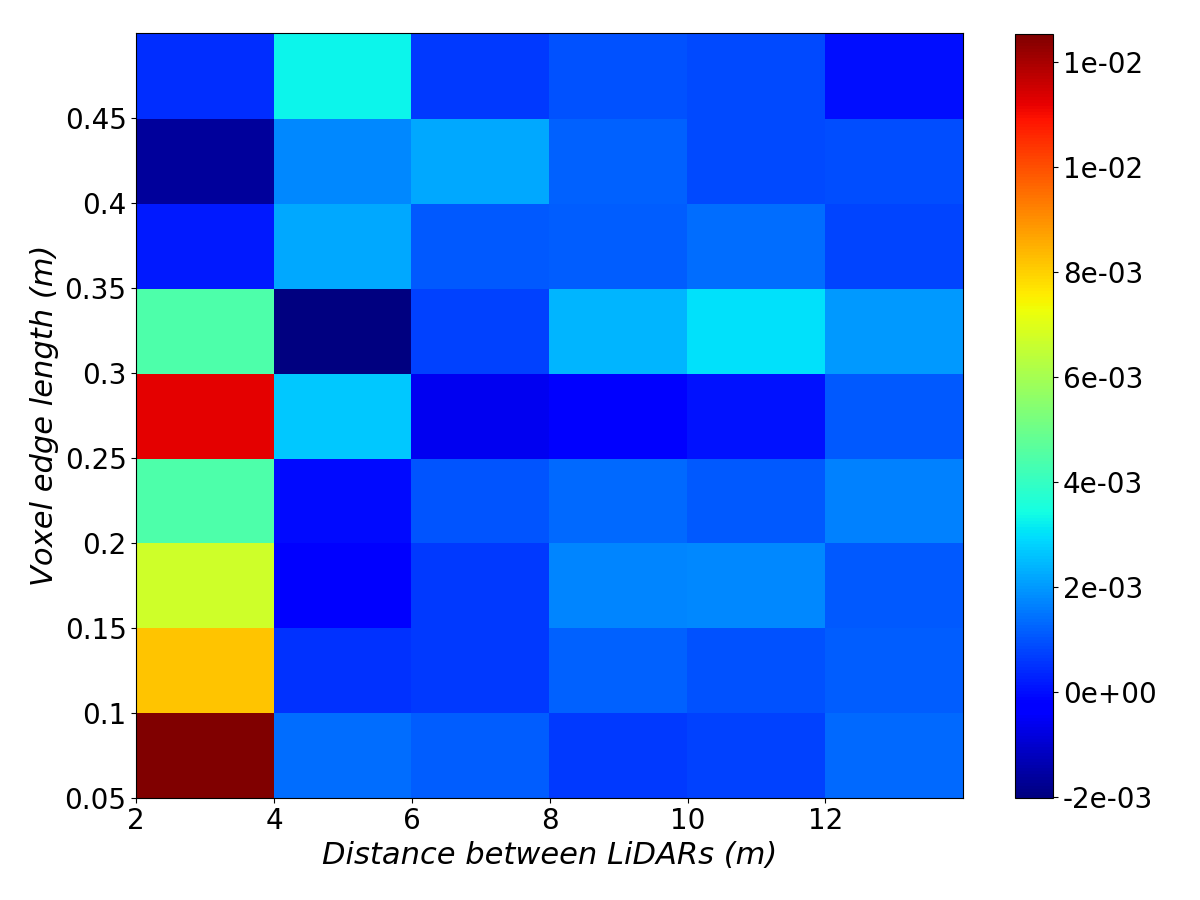
\includegraphics[width=\textwidth]{img/lidar-interference/LOS/octree_difference_color_mesh.png}
	\caption{}%Voxel-to-Voxel analysis results when computing the difference between the results on sub-Figure~(\subref{fig:los:octree-interference-color-mesh}) and sub-Figure~(\subref{fig:los:octree-ground-truth-color-mesh}).}
	\label{fig:los:octree-difference-color-mesh}
\end{subfigure}

\caption[Voxel-to-Voxel analysis when the \acp{lidar} \ac{los} is obstructed and the distance between \acp{lidar} is variated.]{Voxel-to-Voxel \ac{lidar} interference analysis when the parameter under test is the relative distance between the two \acp{lidar}, victim and interferer. In sub-Figure~(\subref{fig:los:octree-interference-color-mesh}), the interfered bag is compared against the ground truth model and in sub-Figure~(\subref{fig:los:octree-ground-truth-color-mesh}), the ground truth bag file is compared with the ground truth model. The latter results are subtracted to the former, resulting in sub-Figure~(\subref{fig:los:octree-difference-color-mesh}). For every sub-figure, the x-axis shows the distance between the \acp{lidar} to which the \acp{lidar} \ac{los} was obstructed, and the y-axis the different values of voxel edge length to which tests were made.}
\label{fig:los:octree-color-mesh}
\end{figure}

Analyzing sub-Figure~\ref{fig:los:octree-interference-color-mesh}, the relative number of modified voxels is 27.5\%, meaning that for a voxel grid size of $\SI{5}{\centi\meter}\times \SI{5}{\centi\meter}\times \SI{5}{\centi\meter}$, 27.5\% of the voxels which contain data were changed. However, comparing this results with the equivalent sub-figure, but which compares the ground-truth model with the ground-truth bag file, sub-Figure~\ref{fig:los:octree-ground-truth-color-mesh}, shows similar results

Despite a small variation of the relative number of modified voxel with the parameter under test (on the x-axis), the rate of change is greater on the y-axis with the increase of the voxel edge length. After a voxel edge length of \SI{0.2}{\meter}, the relative number of interfered voxels tends to stabilize. 

The subtraction between the relative number of modified voxels on the interference and ground truth bags (sub-Figure~\ref{fig:los:octree-difference-color-mesh}), On this image (and corresponding data), in major results of the subtraction are positive, which means that due to interference, the number of changes on the interference bag are greater than on the ground truth bag. The order of magnitude of the number of modified voxels between the two datasets ranges from $10^{-3}$ to $10^{-2}$, which indicates that, on average one in each ten to a hundred voxels has changed its occupation status, due to its points being interfered and wrongly measured.


\subsubsection{Transversal Remarks to all the tests}
Measuring the change detection has performed with the intent to classify, on a more macro-level, how does the interference affect the spatial organization of the point cloud. A voxel tridimensional structure was volume, whereas a point does not; which was believed to be a good analysis to better handle the spatial organization of the point cloud. A better understanding of the spatial organization would allow detecting which regions of the point cloud were affected by interference, which voxels were changed and remain unaffected by interference and how did they change.

However, the results presented do not allow such interpretation. At first, ground truth model generation seems to undermine the results, since it appears that the comparison of the point clouds used to generate the ground truth model yields as many errors as the actual interfered data. Such similarity forced us to double check our implementations, but no mistakes were found. Subtracting one result from the other, while allowing the determination of the order of magnitude that described their differences, resulted in an absence of a clear pattern being found on the data.

After analyzing the data and its results, our understanding is that we underestimate the impact of the \ac{lidar} noise on a voxel representation. If, for a given point near the edge of a voxel, the \ac{lidar} noise causes the measurement of the point to be on another adjacent voxel, a voxel has been modified. Using a small voxel size will magnify the impact of this behavior, since the distance of a point to its voxel limit are smaller. Moreover, a larger voxel size would not solve this situation, since a bigger volume of the point cloud is considered to be interfered. Both situations led to a misrepresentation of the spatial behavior of \ac{lidar} interference. 

From this analysis, we can only conclude that the \ac{lidar} noise is much more significant than previously thought, as it affects the generation of the point cloud model to an extent that severely undermines our capability to make an educated guess about the \ac{lidar} interference behavior and magnitude. On the scenarios presented, our understanding is also that the \ac{lidar} interference seems to be less significant than noise, but further analysis are required before reaching that conclusion with certainty.

The subtraction of the two relative number of changed voxels, when compared with the results in sub-Section~\ref{subsec:lidar-interference:room-outliers-experimental-setup}, reveal a difference of 2 to 3 orders of magnitude, which might be indicative that the impact of \ac{lidar} interference not only has the behavior described in Section~\ref{sec:lidar-interference:room-outliers}, but also interferes with the point measurements similarly to the \ac{lidar} measurement noise.

To deepen this analysis, an approach focused on the point is carried in Section~\ref{sec:lidar-interference:point-to-point-analysis}, which will use the \textit{Frame Registration} method (see sub-Section~\ref{subsec:lidar-interference:frame-registration}) to generate the ground-truth model instead of the \textit{Frame Accumulation} method, used by the voxel-to-voxel analysis.


%%%%%%%%%%%%%%%%%%%%%%%%%%%%%%%%%%%%%%%%%%%%%%%%%%%%%%%%%%%%%%%%%%%%%%%%%%%%%%%%%%%%%%%%%%%%%%%%%
%%%%%%%%%%%%%%%%%%%%%%%%%%%%%%%%%% POINT TO POINT ANALYSIS %%%%%%%%%%%%%%%%%%%%%%%%%%%%%%%%%%%%%%
%%%%%%%%%%%%%%%%%%%%%%%%%%%%%%%%%%%%%%%%%%%%%%%%%%%%%%%%%%%%%%%%%%%%%%%%%%%%%%%%%%%%%%%%%%%%%%%%%

\section{Point-to-Point Analysis}
\label{sec:lidar-interference:point-to-point-analysis}
Point-to-Point analysis quantifies the magnitude of \ac{lidar} interference by counting the amount of points that distance from the ground truth point cloud model by a given threshold. The distance is computed between the point position on the ground truth model and on each of the point cloud frames of the interference bag file, point by point.

Point-to-point analysis relies on the spatial organization of the point cloud structure, which was first introduced in sub-Section~\ref{subsec:lidar-interference:frame-registration}. This data structure organizes an input point cloud, reshaping its data into a matrix structure, similar to a depth image. Each of the matrix indexes corresponds to a \ac{lidar} measurement, being the row index determined by the data \ac{laser} ID and the column index determined by its azimuthal position, which is given in Equation~\eqref{eq:azimuthal-angle-index}. 

By organizing the point cloud of the ground truth model and the point cloud of the interference frame, a direct comparison between two points, that corresponds to the same measurement under different circumstances, can be done. To measure \ac{lidar} interference using point-to-point analysis, the Euclidean distance between the point on the ground truth model and the interference frame, is determined, using Equation~\eqref{eq:euclidian-distance}.

\begin{equation}
\label{eq:euclidian-distance}
\begin{split}
\displaystyle
\text{Euclidean distance} = & \sqrt{(x_{\text{ground\_truth}} - x_{\text{interference\_frame}})^2 + (y_{\text{ground\_truth}} - y_{\text{interference\_frame}})^2} \\
														& \displaystyle \quad \overline{\rule{0pt}{2.5ex} + (z_{\text{ground\_truth}} - z_{\text{interference\_frame}})^2 }
\end{split}
\end{equation}

Repeating this process for all the pairs of points on the organized point clouds, a matrix of depth differences between the ground truth and the interference frame is obtained. This matrix of distances is then serialized\footnote{Data serialization consists on converting a data complex data structure to a stream of bytes, in order to save on file or send. On the case of the depth differences matrix, it means transforming the two-dimensional matrix in a one-dimensional vector.}, generating a vector containing the distance differences. For each interfered point cloud frame from the bag file, the process is repeated and the new vector of distances is appended to the previous one. 

To determine the magnitude of the interference for a specific value of a parameter under test, the distances difference vector, which will be denoted as $d_\text{vec}$, is iterated and the depth difference is compared with a distance threshold, $d_\text{threshold}$. The normalized difference is calculated by dividing the number of interfered points by the total number of points, as detailed in Equation~\eqref{eq:normalized-interference-depth}, where $N$ is the number of elements on the vector, which equals the number of point cloud points on the bag file.

\begin{equation}
\label{eq:normalized-interference-depth}
\displaystyle
\text{Normalized Interference} = \frac{1}{N} \sum\limits^{N-1}_{i = 0} \left(d_{\text{vec}}(i)
> d_\text{threshold}\right)
\end{equation}

\subsection{Implementation}
\texttt{OrganizedPointCloud} is the templated class developed to organize point cloud data. This template version can work with a Velodyne point cloud data type, gathered from the VLP-16, or the abstract \texttt{OrganizedPointCloudContainter}, detailed in sub-Section~\ref{subsec:lidar-interference:frame-registration}, or generic \ac{pcl} point cloud point data types, such as \texttt{PointXYZ}.

The offline \ac{ros} node that performs \textit{Point-to-Point} \ac{lidar} interference analysis relies on this organized point cloud structure for organizing both the ground truth model generated by the algorithm in Section~\ref{sec:lidar-interference:ground-truth-generation}, and each frame of the data under comparison. Using Equation~\eqref{eq:euclidian-distance}, the depth difference matrix is computed by iterating over the two dimensions of the point cloud. 

As detailed in sub-Section~\ref{subsec:lidar-interference:frame-stitching}, the \ac{icp} and Voxel Grid algorithms, despite being templated, cannot maintain the \ac{laser} ID value, therefore, the ground truth model generated by frame stitching cannot be used with this method, since that point cloud does not have the \ac{laser} ID information, required for the spatial organization of the point cloud.

The output of the offline \ac{ros} node is a binary file with the serialized distance between the ground truth model and the interference bag file, for each of the points. Since the organized point cloud dimensions are fixed for each frame, the vector can be reshaped to a tridimensional matrix containing the differences' matrix for each point cloud frame that was compared\footnote{VLP-16 has 16 lasers and rotates at 600 \ac{rpm}. Therefore, each of the depth difference matrix has 16 rows and $\rfrac{\SI{360}{\degree}}{\SI{0.2}{\degree}} = 1800$ points, where \SI{0.2}{\degree} is the angular step of each \ac{lidar} measurement. The vector can be reshaped to a tridimensional matrix of $16\times 1800\times N$, where $N$ is the number of point cloud messages of the bag file.}, but in this case, no gain is obtained for doing so.

This vector of depth differences is loaded by a Python script, specific for the parameter under test, for statistical analysis of the data. Different threshold values are used, with the results being stored on a \ac{csv} file as well as graphical representations of such data. 

\subsection{Results}
\label{subsec:lidar-interference:point-to-point-analysis-results}
The results presented in this sub-Section are based on the comparison of the point cloud, point by point, between the ground truth model and the data with interference. The quality of these results depends, majorly, on two aspects:

\begin{itemize}
\item Correctness of the ground truth model generation algorithm and the generated model;
\item Quality of the interference quantification algorithm.
\end{itemize}

Before dwelling into the results, some considerations must be made regarding the ground truth model. The two algorithms were developed on the premise, as stated in the user guide and datasheet of the Velodyne VLP-16 \ac{lidar}, that the typical distance error a measurement can have, due to sensor noise, is \SI{3}{\centi\meter}~\cite{VLP16}. This means that, when looking at the results caused by \ac{lidar} interference in Section~\ref{subsec:lidar-interference:point-to-point-analysis-results}, we assume that a ``well-behaved'' \ac{lidar}, under interference from another \ac{lidar}, if analyzed using a threshold that is larger than its maximum error, will not exbibit false positives errors due to sensor noise.

Unfortunately, such a reasonable expectation was not met. Our findings reveal not only that the sensor noise is larger than the typical error \SI{3}{\centi\meter} error on a static scenario, as specified on their datasheet,~\cite{VLP16}, but also that, to some extent, \ac{lidar} measurement noise is dominant over the real impact of interference, forbidding us to make an educated assessment of its extent.

We assume that, due to the statistical behavior of measurements, the measurement error of a given distance would be affected by a normal distribution, with mean of \SI{3}{\centi\meter}. Since the standard deviation of the error is not given, we assumed an interval of three sigma, below the normal industry standards of six sigma. An interval of three sigma implies that, given a reasonable threshold such that its value was greater than $3\sigma$ (even not knowing such value) only 0.3\% of the points in the ground truth model would be, theoretically, mistakenly measured as interference when they in fact are noise. Therefore, when analyzing \ac{lidar} data that has been interfered, each point labelled as interfered had a probability of $0.3\%$ of being a false positive, being the erroneous measurement caused by the sensor noise, and not the other \ac{lidar}.

To test our hypotheses, the interference analysis algorithms were also applied to the ground truth bag files, comparing how good the ground truth model was when compared with the point cloud frames that were used to generate it. Our results, as will be detailed next for each of the parameters under test which Point-to-Point analysis was done (distance, height and \ac{los} obstruction), show that when analyzing the ground truth bag for ``interference'', the same order of magnitude is obtained when analyzing the actual interfered bag file. Both bag files where compared against the same ground truth model.

On an attempt to cast a light on such results, we subtract to the normalized number of interference points obtained analyzing the interference bag file the normalized number of erroneous points obtained by analyzing the ground truth bag file. This operation is not intended to be used to obtain direct conclusions, only to help to understanding if the order of magnitude of this difference is similar to the order of magnitude of the interference computed in sub-Section~\ref{subsec:lidar-interference:room-outliers-experimental-setup}. If so, that would indicate that the predominant behavior of the interference is to create outliers that significantly differ from the correct data. If not, \ac{lidar} interference has a more subtle behavior, which can be mistaken by sensor noise, and more advanced techniques of analysis, which separate the two, must be carried to fully study the problem and its behavior.

Subtracting the two normalized interference values assumes that the number of points used to compute this statistical results are statistically representative of the \ac{lidar} measurement noise behavior, which is not fully understood, and may lead to wrong interpretations being made from the data, by basing our observations under false premises. Since we are operating with almost 50 million of points per each value of a parameter under test, we consider that the amount of data being manipulated statistically represents the noise behavior.

\subsubsection{Distance}
For all the distance values (\SIrange{1}{12}{\meter} with a step of \SI{1}{\meter}), the threshold value was varied from \SIrange{0.05}{1.5}{\meter}, with steps of \SI{0.05}{\meter}. The results of the depth differences between the ground truth model and the interference bag are shown in sub-Figure~\ref{fig:distance:interference-color-mesh} and the results of applying the same point-to-point analysis between the ground truth model and the ground truth bag file used to generate it are shown in Figure~\ref{fig:distance:ground-truth-color-mesh}.

\begin{figure}[!ht]
\centering
\begin{subfigure}[c]{0.45\textwidth}
	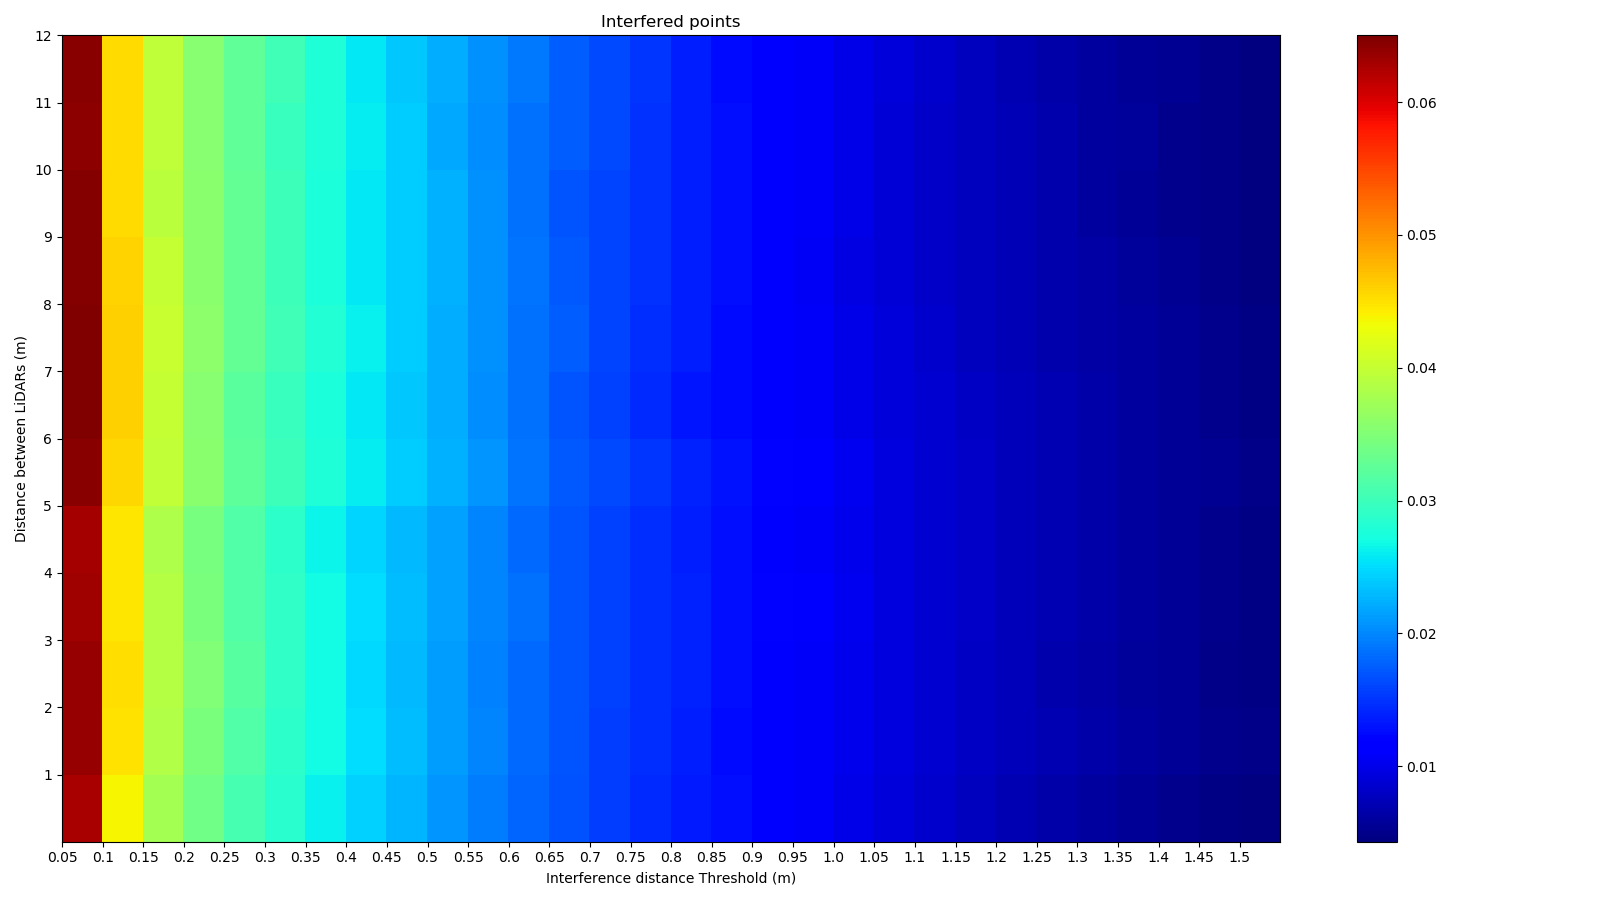
\includegraphics[width=\textwidth]{img/lidar-interference/distance/interference_distance_color_mesh.png}
\caption{}%Point-to-Point analysis results when comparing the interference bag file with the ground truth model.}
	\label{fig:distance:interference-color-mesh}
\end{subfigure}
\qquad
\begin{subfigure}[c]{0.45\textwidth}
	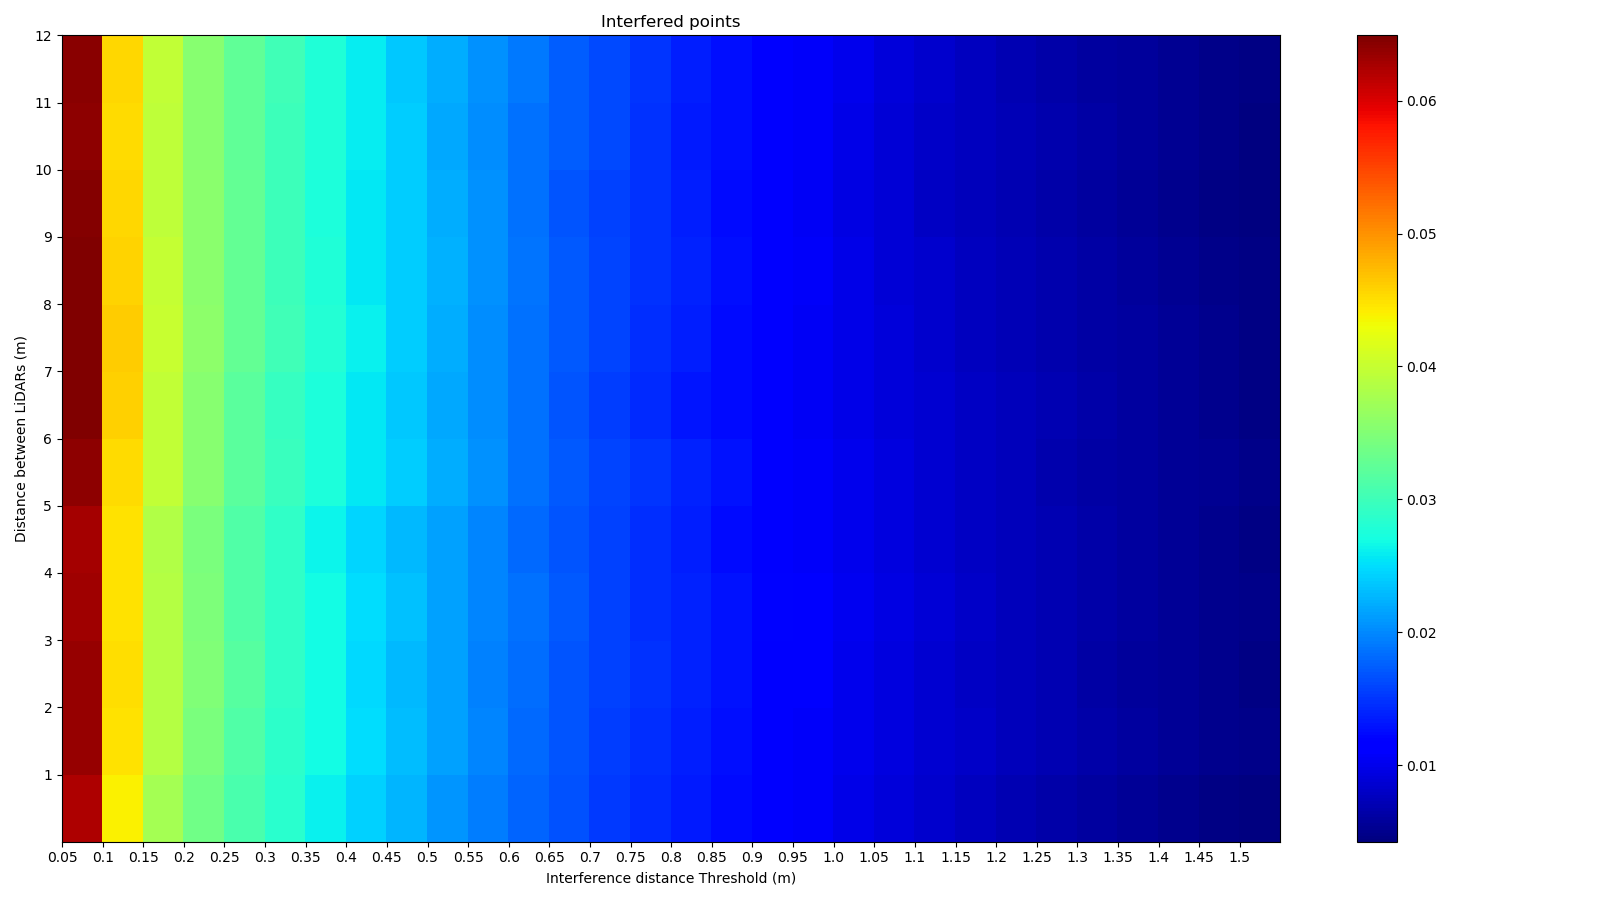
\includegraphics[width=\textwidth]{img/lidar-interference/distance/ground_truth_distance_color_mesh.png}
\caption{}%Point-to-Point analysis results when comparing the ground truth bag file with the ground truth model.}
	\label{fig:distance:ground-truth-color-mesh}
\end{subfigure}
\\ \vspace{4mm}
\begin{subfigure}[c]{0.6\textwidth}
	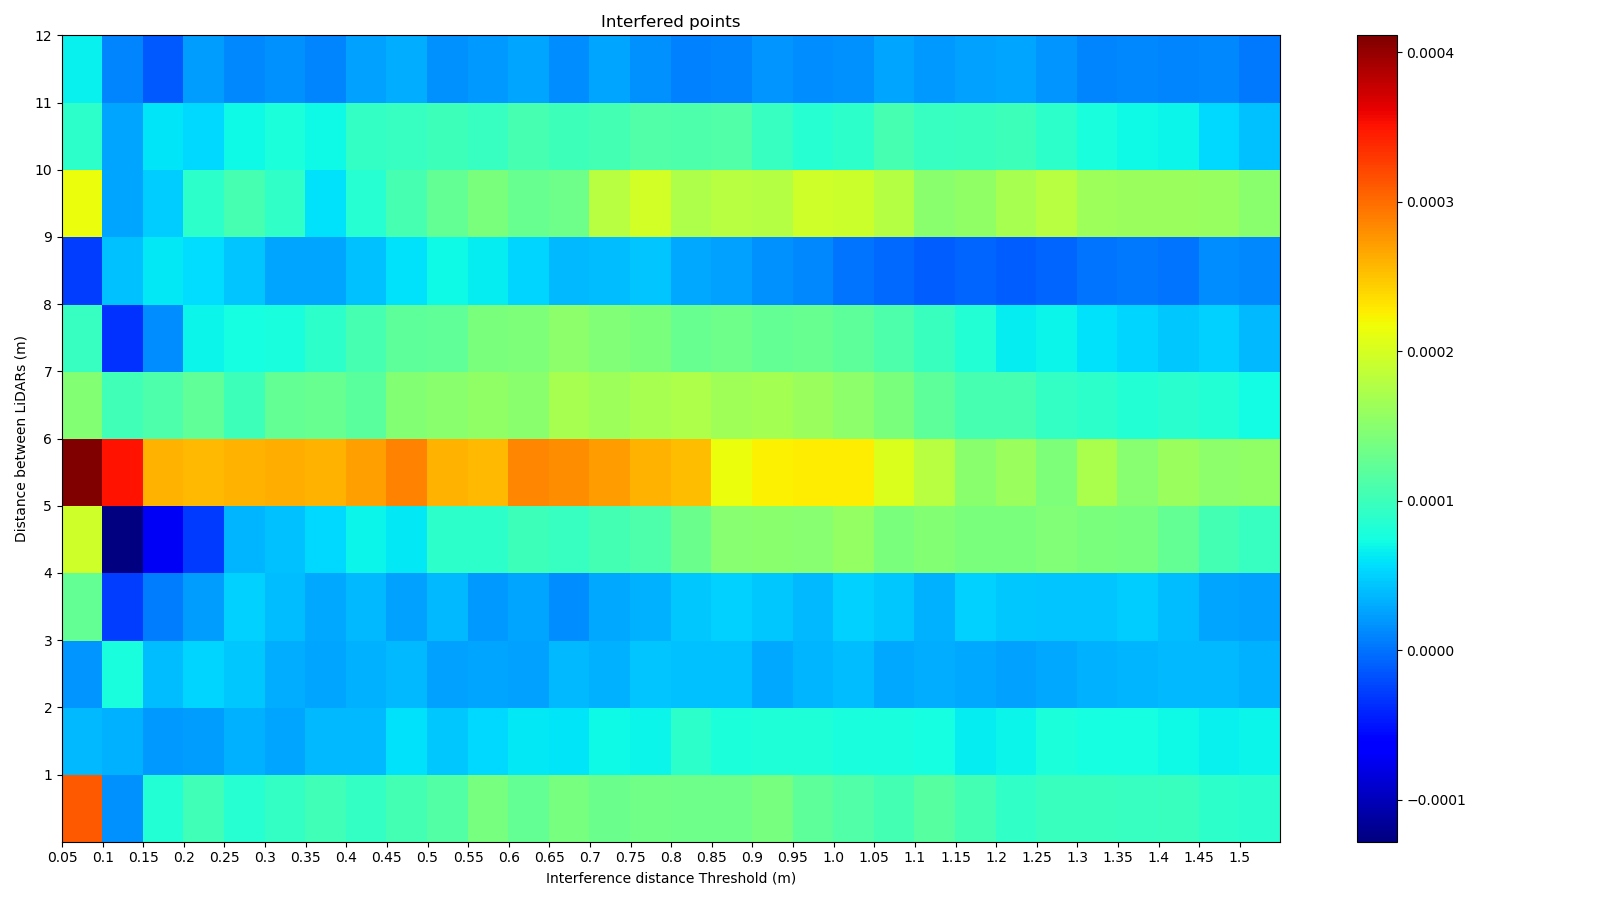
\includegraphics[width=\textwidth]{img/lidar-interference/distance/difference_ground_truth_interference_measurement.png}
\caption{}%Point-to-Point analysis results when computing the difference between the results on sub-Figure~(\subref{fig:distance:interference-color-mesh}) and sub-Figure~(\subref{fig:distance:ground-truth-color-mesh}).}
	\label{fig:distance:difference-color-mesh}
\end{subfigure}

\caption[Point-to-Point analysis when the distance between \acp{lidar} is variated.]{Point-to-Point \ac{lidar} interference analysis when the parameter under test is the relative distance between the two \acp{lidar}, victim and interferer. In sub-Figure~(\subref{fig:distance:interference-color-mesh}), the interfered bag is compared against the ground truth model and in sub-Figure~(\subref{fig:distance:ground-truth-color-mesh}), the ground truth bag file is compared with the ground truth model. The latter results are subtracted to the former, resulting in sub-Figure~(\subref{fig:distance:difference-color-mesh}). For every sub-figure, the x-axis shows the threshold distance at which a depth difference is considered an interference and the y-axis shows the different values of distance, the parameter under test.}
\label{fig:distance:color-mesh}
\end{figure}

Analyzing Figure~\ref{fig:distance:color-mesh}, the normalized interference variation between the maximum and minimum values is almost 7 times. However, the metric used to analyze the interference, the distance threshold value between the ground truth model and its corresponding point on the bag file under test which classifies a point is being interfered, has more impact on the interference value than the parameter under test (distance between \ac{lidar}). The range of variation is wider along the x-axis, which contains the distance threshold, than along the y-axis, that variates the parameter under test. Sub-figures~\ref{fig:distance:interference-color-mesh} and~\ref{fig:distance:ground-truth-color-mesh} are practically similar, with its reason being described in the beginning of this sub-Section.

The subtraction between the normalized interference on the interference and ground truth bag files, shown in sub-Figure~\ref{fig:distance:difference-color-mesh}, reveals the order of magnitude of the interference: $10^{-4}$. As detailed in the beginning of the sub-Section, we assume, due to the number of points used on these statistical analysis, that they are statistically representative of the noise associated with the \ac{lidar} measurements, therefore the difference between the two results (ground truth model vs. ground truth bag and ground truth model vs. interference bag), if the noise was the same magnitude on both, would reveal the magnitude of the interference. 

Comparing this magnitude with the results in Figure~\ref{fig:box-filter-outliers-distance}, whose magnitude varies from $10^{-7}$ to $10^{-5}$, the total number of interfered points for the distance scenario, using a point-to-point analysis is 1 to 3 orders of magnitude greater than the normalized number of outliers outside the room dimensions (which are clearly caused by interference), detailed in sub-Section~\ref{subsec:lidar-interference:room-outliers-experimental-setup}. Therefore, we can conclude that on this scenario, the majority of interference is present inside the room dimensions, and not outside.

\subsubsection{Height}
For all the relative height values between the two \acp{lidar} (\SIlist[list-units=single]{0.623; 0.715; 0.818; 0.931; 1.032; 1.144; 1.277}{\meter}), the threshold value was varied from \SIrange{0.05}{1.5}{\meter}, with steps of \SI{0.05}{\meter}. The results of the depth differences between the ground truth model and the interference bag are shown in sub-Figure~\ref{fig:height:interference-color-mesh} and the results of applying the same point-to-point analysis between the ground truth model and the ground truth bag file used to generate it are shown in Figure~\ref{fig:height:ground-truth-color-mesh}.

\begin{figure}[!ht]
\centering
\begin{subfigure}[c]{0.45\textwidth}
	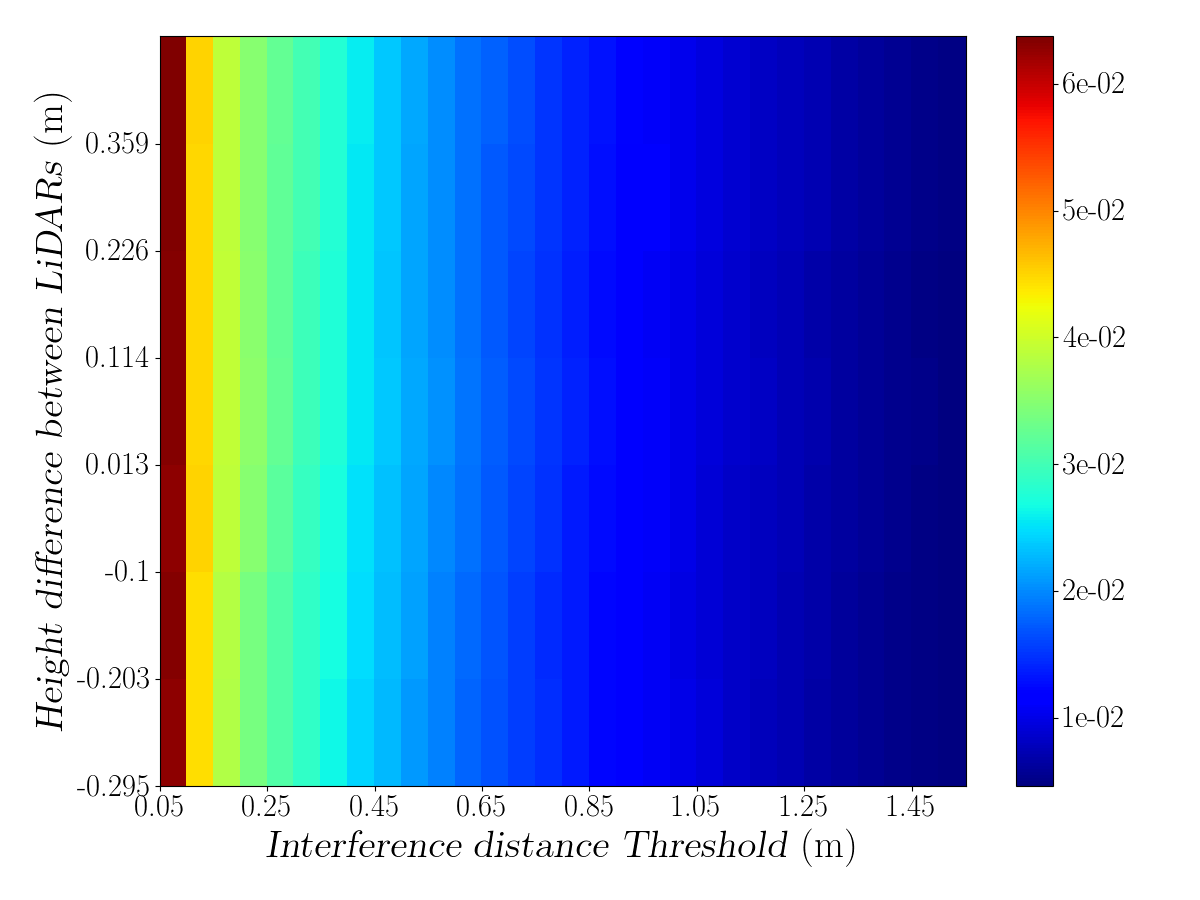
\includegraphics[width=\textwidth]{img/lidar-interference/height/interference_distance_color_mesh.png}
\caption{}%Point-to-Point analysis results when comparing the interference bag file with the ground truth model.}
	\label{fig:height:interference-color-mesh}
\end{subfigure}
\qquad
\begin{subfigure}[c]{0.45\textwidth}
	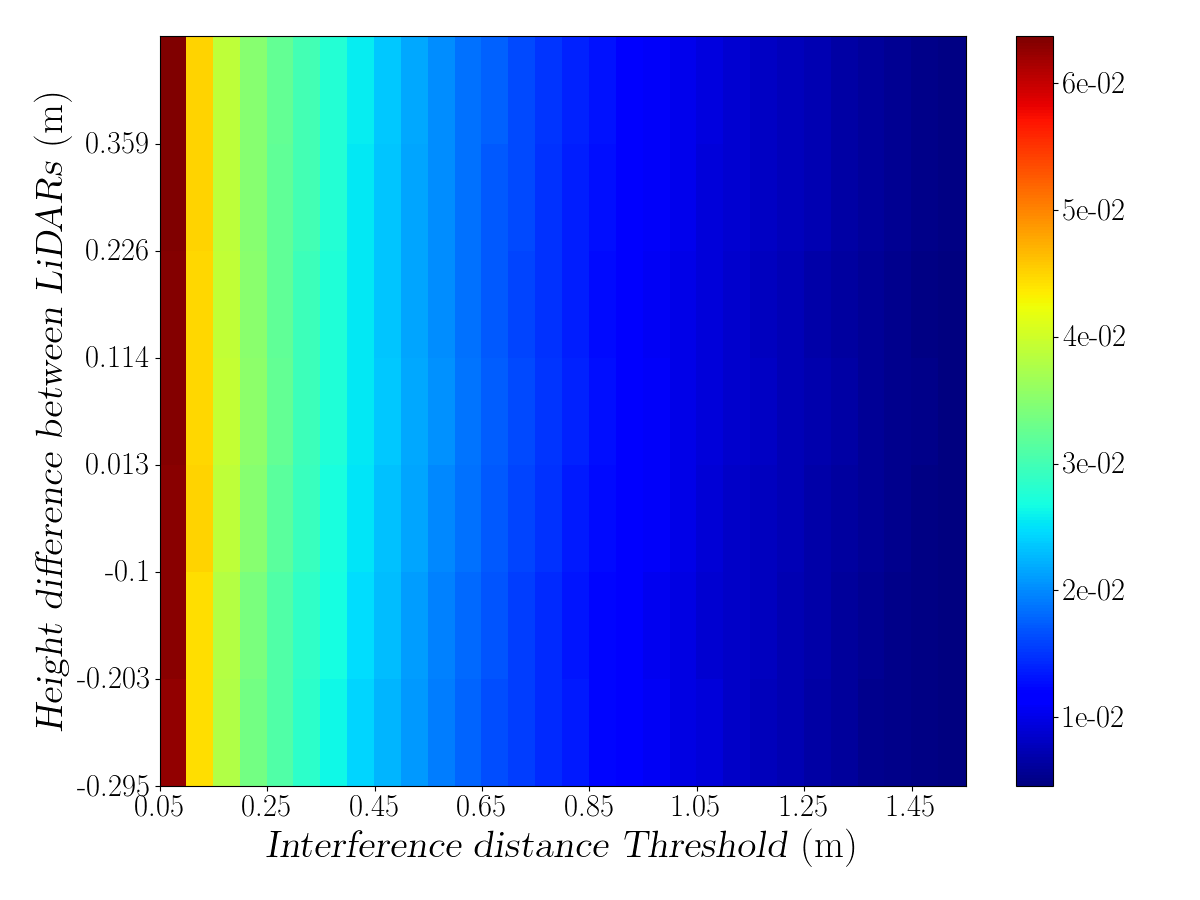
\includegraphics[width=\textwidth]{img/lidar-interference/height/ground_truth_distance_color_mesh.png}
\caption{}%Point-to-Point analysis results when comparing the ground truth bag file with the ground truth model.}
	\label{fig:height:ground-truth-color-mesh}
\end{subfigure}
\\ \vspace{4mm}
\begin{subfigure}[c]{0.6\textwidth}
	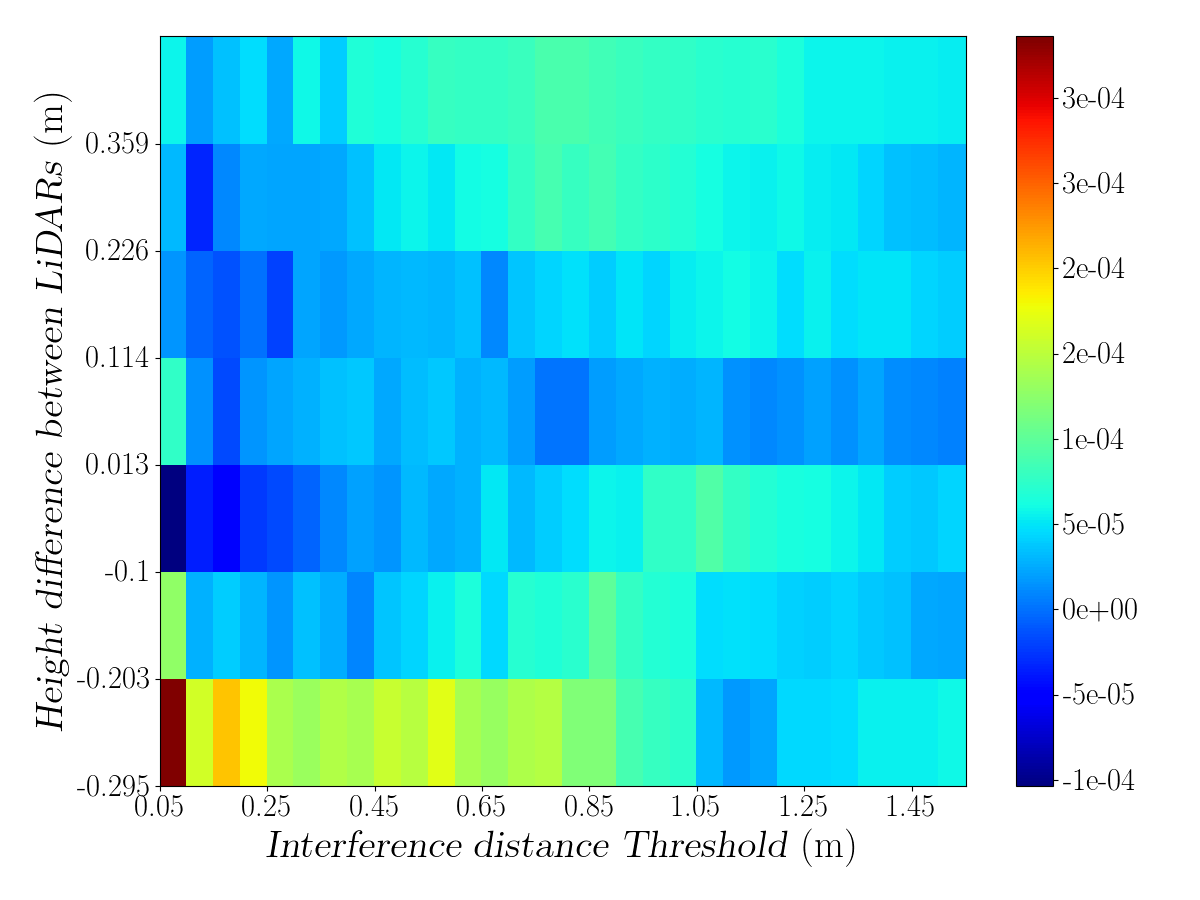
\includegraphics[width=\textwidth]{img/lidar-interference/height/difference_ground_truth_interference_measurement.png}
\caption{}%Point-to-Point analysis results when computing the difference between the results on sub-Figure~(\subref{fig:height:interference-color-mesh}) and sub-Figure~(\subref{fig:height:ground-truth-color-mesh}).}
	\label{fig:height:difference-color-mesh}
\end{subfigure}

\caption[Point-to-Point analysis when the relative height  between \acp{lidar} optical center is variated.]{Point-to-Point \ac{lidar} interference analysis when the parameter under test is the relative distance between the two \acp{lidar}, victim and interferer. In sub-Figure~(\subref{fig:height:interference-color-mesh}), the interfered bag is compared against the ground truth model and in sub-Figure~(\subref{fig:height:ground-truth-color-mesh}), the ground truth bag file is compared with the ground truth model. The latter results are subtracted to the former, resulting in sub-Figure~(\subref{fig:height:difference-color-mesh}). For every sub-figure, the x-axis shows the threshold distance at which a depth difference is considered an interference and the y-axis shows the different values of relative height between the \acp{lidar}, the parameter under test.}
\label{fig:height:color-mesh}
\end{figure}


In Figure~\ref{fig:height:color-mesh}, considerations previously made remain valid: the metric used to analyze the interference (the distance threshold value) has more impact on the interference value than the parameter under test, as can be seen on sub-figures~(\subref{fig:height:ground-truth-color-mesh}) and (\subref{fig:height:interference-color-mesh}). Refer to the beginning of this sub-Section (\ref{subsec:lidar-interference:point-to-point-analysis-results}), for a detailed explanation on the reason for similarities between these two sub-figures. 

The difference between their normalized interference, shown in sub-Figure~\ref{fig:height:difference-color-mesh}, indicates an interference on the order of magnitude of $10^{-4}$ to $10^{-5}$. As detailed in the beginning of the sub-Section~\ref{subsec:lidar-interference:point-to-point-analysis-results}, the noise represented on the ground truth bag file (sub-Figure~\ref{fig:height:ground-truth-color-mesh}) is assumed to be statistically representative of the noise associated with the \ac{lidar} measurements, therefore the difference between the two results (ground truth model vs. ground truth bag and ground truth model vs. interference bag), reveals the magnitude of the interference. 

Comparing this magnitude ($10^{-4}$) with the results presented in Figure~\ref{fig:box-filter-outliers-height}, which are on the order of magnitude of $10^{-6}$, the normalized number of interfered points resulting from varying the relative height between the two \acp{lidar}, using point by point analysis is 1 to 2 orders of magnitude larger than the normalized number of outliers outside the room dimensions (which are clearly caused by interference), depicted on the bar chart of Figure~\ref{fig:box-filter-outliers-height}

\subsubsection{\acp{lidar} \acl{los} Obstruction}
For all the distances that the \acf{los} between the two \acp{lidar} was obstructed (\SIrange{2}{12}{\meter} with steps of \SI{2}{\meter}), the interference magnitude was analyzed with a varying threshold value, from \SIrange{0.05}{1.5}{\meter}, with steps of \SI{0.05}{\meter}. The results of the depth differences between the ground truth model and the interference bag are shown in sub-Figure~\ref{fig:los:interference-color-mesh} and the results of applying the same point-to-point analysis between the ground truth model and the ground truth bag file used to generate the ground truth model are shown in Figure~\ref{fig:los:ground-truth-color-mesh}.

\begin{figure}[!ht]
\centering
\begin{subfigure}[c]{0.45\textwidth}
	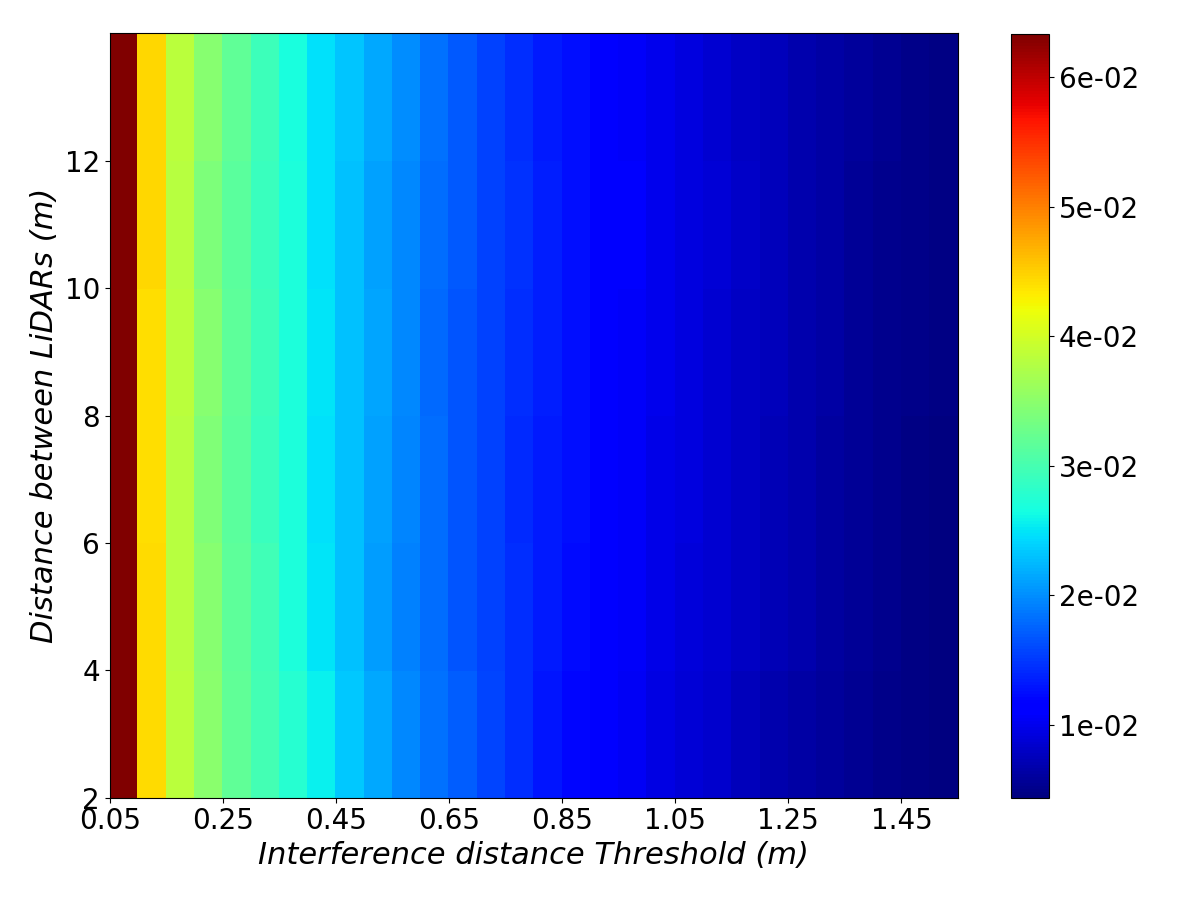
\includegraphics[width=\textwidth]{img/lidar-interference/LOS/interference_distance_color_mesh.png}
\caption{}%Point-to-Point analysis results when comparing the interference bag file with the ground truth model.}
	\label{fig:los:interference-color-mesh}
\end{subfigure}
\qquad
\begin{subfigure}[c]{0.45\textwidth}
	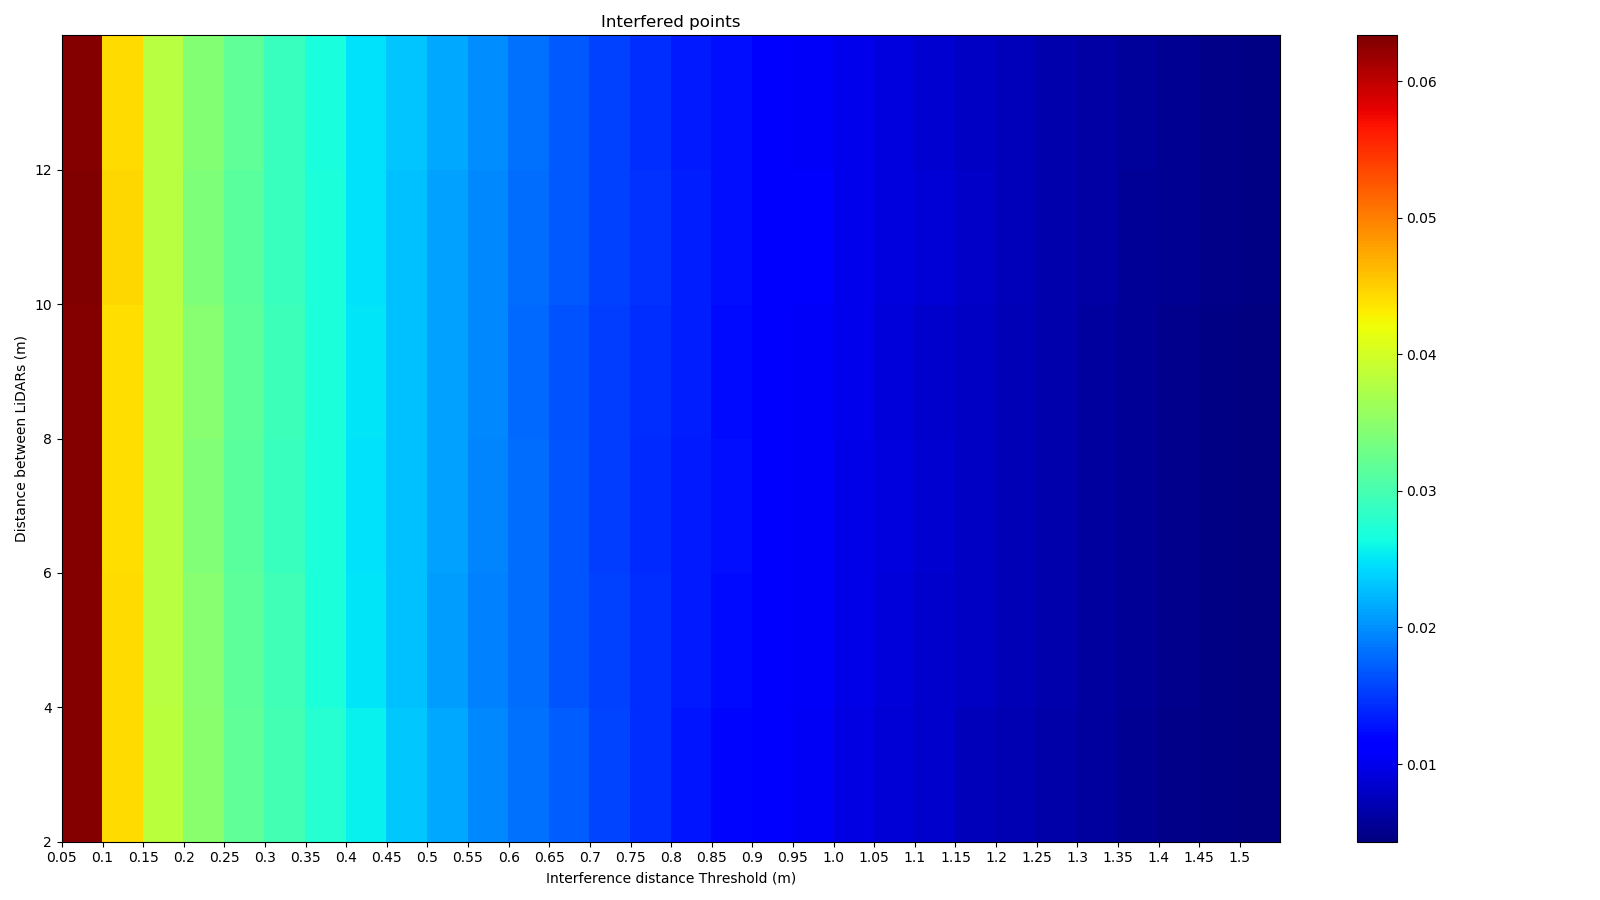
\includegraphics[width=\textwidth]{img/lidar-interference/LOS/ground_truth_distance_color_mesh.png}
\caption{}%Point-to-Point analysis results when comparing the ground truth bag file with the ground truth model.}
	\label{fig:los:ground-truth-color-mesh}
\end{subfigure}
\\ \vspace{4mm}
\begin{subfigure}[c]{0.6\textwidth}
	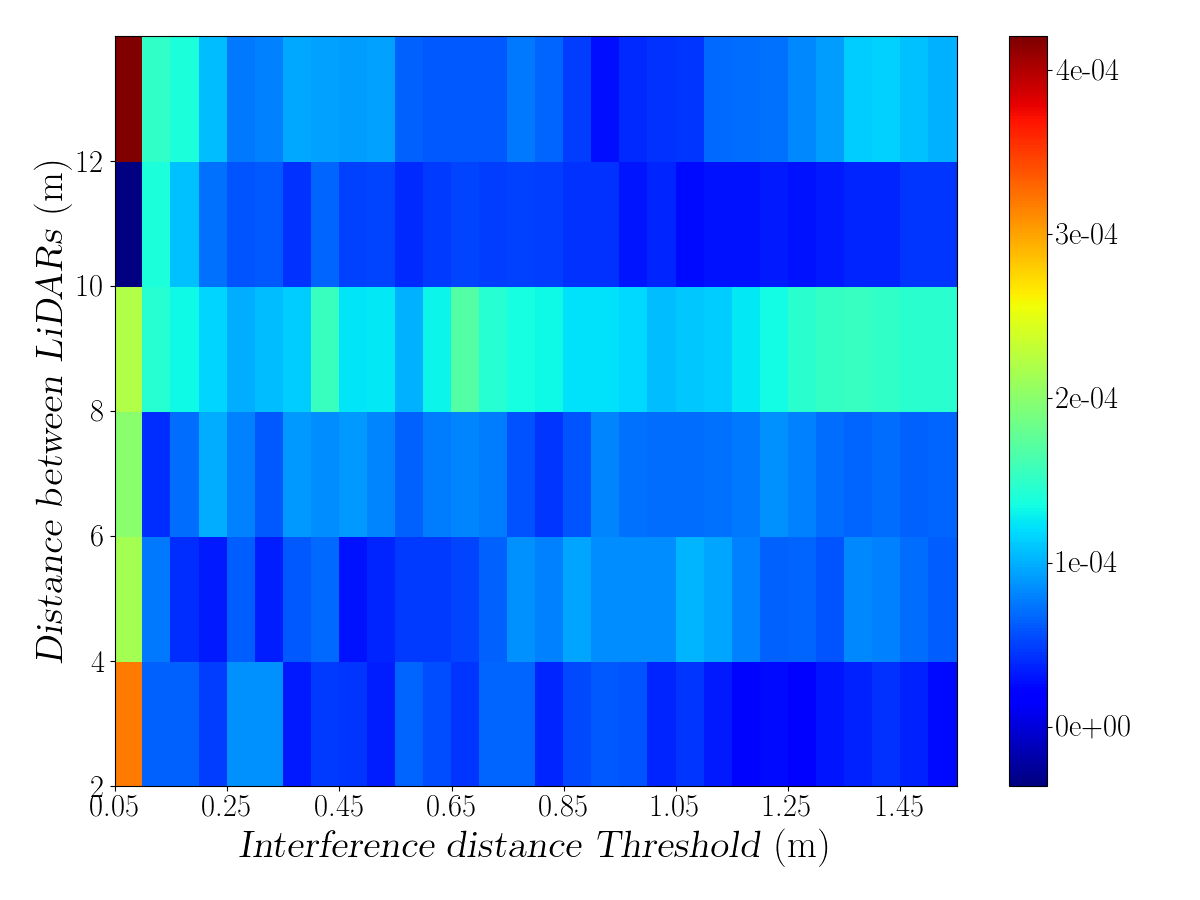
\includegraphics[width=\textwidth]{img/lidar-interference/LOS/difference_ground_truth_interference_measurement.png}
\caption{}%Point-to-Point analysis results when computing the difference between the results on sub-Figure~(\subref{fig:los:interference-color-mesh}) and sub-Figure~(\subref{fig:los:ground-truth-color-mesh}).}
	\label{fig:los:difference-color-mesh}
\end{subfigure}

\caption[Point-to-Point analysis when the \ac{los} between the \acp{lidar} is obstructed and their relative distance is  variated.]{Point-to-Point \ac{lidar} interference analysis when the parameter under test is the relative distance between the two \acp{lidar}, victim and interferer. In sub-Figure~(\subref{fig:los:interference-color-mesh}), the interfered bag is compared against the ground truth model and in sub-Figure~(\subref{fig:los:ground-truth-color-mesh}), the ground truth bag file is compared with the ground truth model. The latter results are subtracted to the former, resulting in sub-Figure~(\subref{fig:los:difference-color-mesh}). For every sub-figure, the x-axis shows the threshold distance at which a depth difference is considered an interference and the y-axis shows the different values of the distance between the two \acp{lidar}, the parameter under test, with the obstacle that blocks their \ac{los} being placed at the medium distance between the two.}
\label{fig:los:color-mesh}
\end{figure}

Analyzing Figure~\ref{fig:los:color-mesh}, the metric used to analyze the interference (the distance threshold value), has more impact on the interference value than the parameter under test (distance between \ac{lidar}, when their \ac{los} is being obstructed), as verified also for the previous parameters under test. Sub-figures~\ref{fig:los:interference-color-mesh} and~\ref{fig:los:ground-truth-color-mesh} are practically similar, as described in the beginning of this sub-Section (see~\ref{subsec:lidar-interference:point-to-point-analysis-results}).

The subtraction of their normalized interference, shown in sub-Figure~\ref{fig:height:difference-color-mesh}, indicates an interference on the order of magnitude of $10^{-4}$. As detailed in the beginning of the sub-Section, we assume, due to the number of points used on these statistical analysis, that they are statistically representative of the noise associated with the \ac{lidar} measurements. Therefore, the difference between the two results (ground truth model vs. ground truth bag and ground truth model vs. interference bag), if the noise was the same magnitude on both, would reveal the magnitude of the interference. 

Comparing this magnitude with the results in Figure~\ref{fig:box-filter-outliers-LOS}, whose magnitude varies from $10^{-7}$ to $10^{-6}$, the total number of interfered points for a \ac{los} obstruction scenario, with the distance between the two \acp{lidar} being varied, using point by point analysis is from 2 to 3 orders of magnitude larger than the normalized number of outliers outside the room dimensions (which are clearly caused by interference).


\subsubsection{Transversal Remarks to all the tests}
Comparing sub-figures (a) and (b), from figures~\ref{fig:distance:color-mesh},~\ref{fig:height:color-mesh} and~\ref{fig:los:color-mesh} we notice that their general aspect is similar, despite the values for each cell being different, revealing the metric chosen for analysis, the distance threshold, has
more impact than the parameter under test (distance between sensors, height or \ac{los} obstruction) whose values are being varied. Another hypothesis is, due to the difference of sub-figures~\ref{fig:distance:difference-color-mesh},~\ref{fig:height:difference-color-mesh} and~\ref{fig:los:difference-color-mesh}, that the impact of the noise on the data is more relevant than the interference between \acp{lidar}. Therefore, since the number of points is statistically representative of the noise phenomenon, the sub-figure (a) and (b) look similar, but when the impact of the noise is ``removed'', the underlying interference behavior is revealed. 

This interference behavior has an order of magnitude that is contained between $10^{-4}$ to $10^{-5}$, which in the all range of the data analyzed, is one to three orders of magnitude greater than the results obtained in sub-Section~\ref{subsec:lidar-interference:room-outliers-experimental-setup}, which only considers the interference that is outside of the room dimensions. Our analysis reveals that such magnitude is a good minorant for the \ac{lidar} interference, but the major part of this interference has a more subtle behavior, affecting slightly the measurements of each point.

Regarding the colormap scale, to the right of each image, its lowest scale value contains negative values, that have the same order of magnitude than the positive ones. Those results indicate that the ground truth bag, which was used to generate the ground truth model, is more poorly related to the model it generates than the interference bag. Two explanations are possible for such behavior:

\begin{enumerate}
	\item Since the interference bag file is recorded with the triple of the duration of the ground truth bag file, the effects of interference and noise are ``diluted'' during normalization, due to the larger number of points;
	\item Due to an unforeseen  combination of some parameters, the interference effect on the point distance counteracted the noise, resulting in the point being contained inside the threshold limits.
\end{enumerate}

Accepting the first hypothesis as valid implies that the number of points contained on the bag files are not statistically representative of the \ac{lidar} measurement noise phenomena, which is the premise upon all this analysis is carried. If the number of points under test changes the value of the normalized interference, then the number of points being used is not enough to statistically represent the phenomena, and we cannot subtract the error measurements to obtain the order of magnitude of the interference.

Also, if we analyze the sub-figures (a) and (b), from figures~\ref{fig:distance:color-mesh},~\ref{fig:height:color-mesh} and~\ref{fig:los:color-mesh}, their overall trend is similar, which indicates that they represent with accuracy the noise phenomena, otherwise some variations among them would be seen, due to the magnitude of \ac{lidar} measurement noise.

The second hypothesis seems far-fetched, but considering that the normalized point cloud interference is on the order of $10^{-4}$, it only requires 3 points\footnote{Considering the typical VLP-16 point cloud with 28800 points, the number of points which have been interfered are: $\approx 10^{-4} \times 28800 = 2.88$.} to be possible.



%%%%%%%%%%%%%%%%%%%%%%%%%%%%%%%%%%%%%%%%%%%%%%%%%%%%%%%%%%%%%%%%%%%%%%%%%%%%%%%%%%%%%%%%%%%%%%%%%
%%%%%%%%%%%%%%%%%%%%%%%%%%%%%%%%%%%%% INTERFERENCE ON ROI %%%%%%%%%%%%%%%%%%%%%%%%%%%%%%%%%%%%%%%
%%%%%%%%%%%%%%%%%%%%%%%%%%%%%%%%%%%%%%%%%%%%%%%%%%%%%%%%%%%%%%%%%%%%%%%%%%%%%%%%%%%%%%%%%%%%%%%%%

\section{Interference on \acp{roi}}
\label{sec:lidar-interference:interference-roi}
The previous analysis on \ac{lidar} interference considers only outliers (Section~\ref{sec:lidar-interference:room-outliers}), voxel occupation change (Section~\ref{sec:lidar-interference:voxel-analysis}) or the distance between points in a point-to-point analysis in the entire point cloud (Section~\ref{sec:lidar-interference:point-to-point-analysis}). In this section we offer a complementary analysis, based on a point-to-point analysis of the interference, but focusing on specific objects of interest.

This analysis is possible due to the outcomes of Chapter~\ref{chapter:object-detection}, which allow the determination of correspondences between \acp{roi} detected on the image and their corresponding points on the point cloud. From such correspondences, we can select a \ac{roi} on the point cloud, generate its ground truth from non-interfered data and compare the model with the interfered point cloud frames.

However, on our experimental datasets, detailed in Section~\ref{sec:lidar-interference:experimental-setup}, the possible objects of interest are further away from the \ac{lidar}. With a polar angular step between lasers of \SI{2}{\degree}, at \SI{3}{\meter} from the \ac{lidar}, there is a vertical distance of \SI{10}{\centi\meter} between each laser scan. At \SI{5}{\meter}, where some detected objects are present, that distance is of \SI{17.4}{\centi\meter} and at \SI{12}{\meter}, where the human dummy is located\footnote{Please note that an obvious solution would be to take measurements with the dummy closer to the camera, on the scenarios described in~\ref{subsec:lidar-interference:parameters-under-test}. Such solution was not possible due to the dummy belonging to another experiment and unavailable for being moved.}, we expect a vertical distance between \ac{lidar} \ac{laser} scans of \SI{42}{\centi\meter}, totalling only 3 lines of data for the human dummy.

To tackle this issue, already expected, a different dataset was previously recorded, codenamed \textit{Human}. A standing person was positioned for being detected by the camera and \ac{lidar}. Its position on the \ac{lidar} coordinates are detailed in Table~\ref{tab:human-position}, and the interferer \ac{lidar} distance to the target value was varied from~\SIrange{3}{6}{\meter}, with steps of \SI{1}{\meter}. Other conditions were similar to the distance test: optical centers aligned and the azimuthal angular position between the two close to zero.

\begin{table}[!ht]
	\centering
	\renewcommand{\arraystretch}{1.2}
	\begin{tabular}{@{}C{3cm}c@{}}
		\toprule
	  Coordinate & Value \\
		\midrule
		x & \SI{5.01}{\meter} \\
		y & \SI{-1.02}{\meter} \\
		$z_\text{min}$ & \SI{-0.956}{\meter} \\
		$z_\text{max}$ & \SI{0.88}{\meter} \\
		\bottomrule
	\end{tabular}
	\caption[Person position in relation to the \ac{lidar} coordinate frame on the \textit{Human} dataset.]{Person position in relation on the \ac{lidar} coordinate frame on the \textit{Human} dataset. Note that the \ac{lidar} axis, x is forward, y is leftwards and z is upwards. $z_\text{min}$ is the position of the feet and $z_\text{max}$ the top of the head.}
	\label{tab:human-position}
\end{table}

In Figure~\ref{fig:human-test-scenario}, an example of the test scenario, taken by the camera, is presented. The interferer \ac{lidar} is positioned at a distance of~\SI{6}{\meter} from its victim, VLP-16, with their optical centers aligned and a near zero azimuthal angle difference.

\begin{figure}[!ht]
	\centering
	\includegraphics[width=0.6\textwidth]{img/lidar-interference/human/test-scenario-white-balanced.png}
	\caption[Test scenario for analyzing the \ac{lidar} interference in \acp{roi}.]{Example of the \textit{Human} test scenario, used for analyzing the \ac{lidar} interference in \acp{roi}. The HESAI Pandar 40 \ac{lidar}, for the test scenario being shown, is placed at a distance of \SI{6}{\meter} from Velodyne VLP-16 and the person position is indicated in Table~\ref{tab:human-position}. A soccer ball, a chair and a human dummy are also present on the image.}
	\label{fig:human-test-scenario}
\end{figure}

\subsection{Implementation}
\label{subsec:lidar-interference:roi-implementation}
To analyze the interference on the selected \ac{roi} we opt to reuse the previous algorithms for ground truth generation (see Frame Registration, in sub-Section~\ref{subsec:lidar-interference:frame-registration}) and interference analysis (see Point-to-Point Analysis, in Section~\ref{sec:lidar-interference:point-to-point-analysis}), which are both implemented as offline nodes. Therefore, the results of the object detection and point cloud bounding box estimation applied to the \textit{Human} dataset must be recorded to a bag file, so that it can be loaded by \texttt{ground\_truth\_model\_estimation\_node} and \texttt{point\_cloud\_interference\_analysis\_node}.

The recording apparatus is shown in Figure~\ref{fig:human-roi-generation}, on Appendix~\ref{appendix:appendix-diagrams}. From the camera intrinsic calibration parameters and the image, the \texttt{darknet\_ros} detects the objects. \texttt{correspondences\_finder} determines the point cloud points that belong to the object(s) on the \acp{roi}, \texttt{point\_cloud\_clusters}, required for \ac{lidar} interference analysis using Point-to-Point Analysis. It uses the point cloud data (\texttt{/velodyne\_point}), the rigid body transform between the camera and \ac{lidar} (\texttt{/camera\_to\_velodyne}) and the image bounding boxes information.


%\begin{figure}[!ht]
%	\centering
%	\def\svgwidth{\columnwidth}
%	\graphicspath{{img/lidar-interference/human/}}
%	\includesvg{img/lidar-interference/human/human-roi-generation-print}
%	\caption[\ac{ros} node graph to implement the \acp{roi} recording for later analysis.]{\ac{ros} node graph representing the nodes and their interactions to generate and record the point cloud clusters corresponding to the \ac{roi}'s in the image. \texttt{Rosbag\_Player} is responsible for playing the dataset data; \texttt{darknet\_ros} for computing the image bounding boxes and \texttt{correspondences\_finder} the point cloud corresponding to the object on the \ac{roi}. \texttt{/Bag\_Recorder} is a \ac{ros} bag record to save the data generated into a bag file.}
%	\label{fig:human-roi-generation}
%\end{figure}

As detailed in sub-Section~\ref{subsec:object-detection:bounding-boxes-and-roi}, the clustering algorithm can be tuned to filter the undesired data using three parameters. Those parameters were previously tuned for \ac{kitti} dataset, in order to select the road vehicles on the image as the objects of interest. On \ac{irislab} \textit{Human} dataset, the only object of interest present on the image is the person, and so the parameters are adjusted to remove all the points from the \ac{roi} that do not belong to the person. 

These parameters were fine-tuned using the dynamic reconfigure capabilities of the \texttt{correspondences\_finder\_node}, and the process to fine-tune the parameters, previously done for \ac{kitti}'s dataset was repeated (refer to sub-Section~\ref{subsec:object-detection:bounding-boxes-and-roi} for more details). The final results for the parameters are given in Table~\ref{tab:experimental-euclidian-cluster-specs}, were the \textit{Maximum cluster size} parameter was not modified.


\begin{table}[!ht]
	\centering
	\renewcommand{\arraystretch}{1.2}
	\begin{tabular}{@{}p{6cm}l@{}}
	 \toprule
	 Specification & Value \\
	 \midrule
	 Cluster Distance Tolerance & \SI{0.50}{\meter} \\
	 Minimum cluster size & $40$ \\
	 Maximum cluster size & $8000$ \\
	 \bottomrule
	\end{tabular}
	\caption[Euclidian cluster parameters to select only the \ac{roi} containing the person on the \textit{Human} dataset.] {\texttt{correspondences\_finder\_node} parameters for the \ac{pcl}'s Euclidean Cluster filter. On the data recorded for the \textit{Human} dataset, these parameters allow the detection of the person while removing all the other objects of interest detected on the image}.
	\label{tab:experimental-euclidian-cluster-specs}
\end{table}

\subsection{Results}
To establish a comparison between the \ac{lidar} interference analysis on \ac{roi} on the point cloud, first a Point-to-Point analysis is applied on all the frames of the bag files, similarly to the work presented in sub-Section~\ref{subsec:lidar-interference:point-to-point-analysis-results}.

Using the algorithm detailed in sub-Section~\ref{subsec:lidar-interference:roi-implementation}, the bag files containing the point cloud points for the clusters on the \acp{roi} are generated, their ground truth models computed using \textit{Frame Registration} (see sub-Section~\ref{subsec:lidar-interference:frame-registration}) and analyzed used Point-to-Point analysis algorithm. After both analysis, done with the same algorithms, are completed, some remarks are given and the results are compared.

\subsubsection{Without \ac{roi} extraction}
With the person placed on the \ac{lidar} coordinate frame at (\SI{5.01}{\meter}, \SI{-1.02}{\meter}), the distance between the two \acp{lidar} was incremented from \SIrange{3}{6}{\meter}, with steps of \SI{1}{\meter}, measured in the same conditions as the distance test (see sub-Section~\ref{subsec:lidar-interference:parameters-under-test} for more details). 

The interference magnitude was analyzed with a varying distance threshold value, from \SIrange{0.05}{0.5}{\meter}, with steps of \SI{0.05}{\meter}. The results of the depth differences between the ground truth model and the interference bag are shown in sub-Figure~\ref{fig:human:interference-color-mesh} and the results of applying the same point-to-point analysis between the ground truth model and the ground truth bag file used to generate the ground truth model are shown in Figure~\ref{fig:human:ground-truth-color-mesh}.

\begin{figure}[!ht]
	\centering
	\begin{subfigure}[c]{0.45\textwidth}
		\centering
		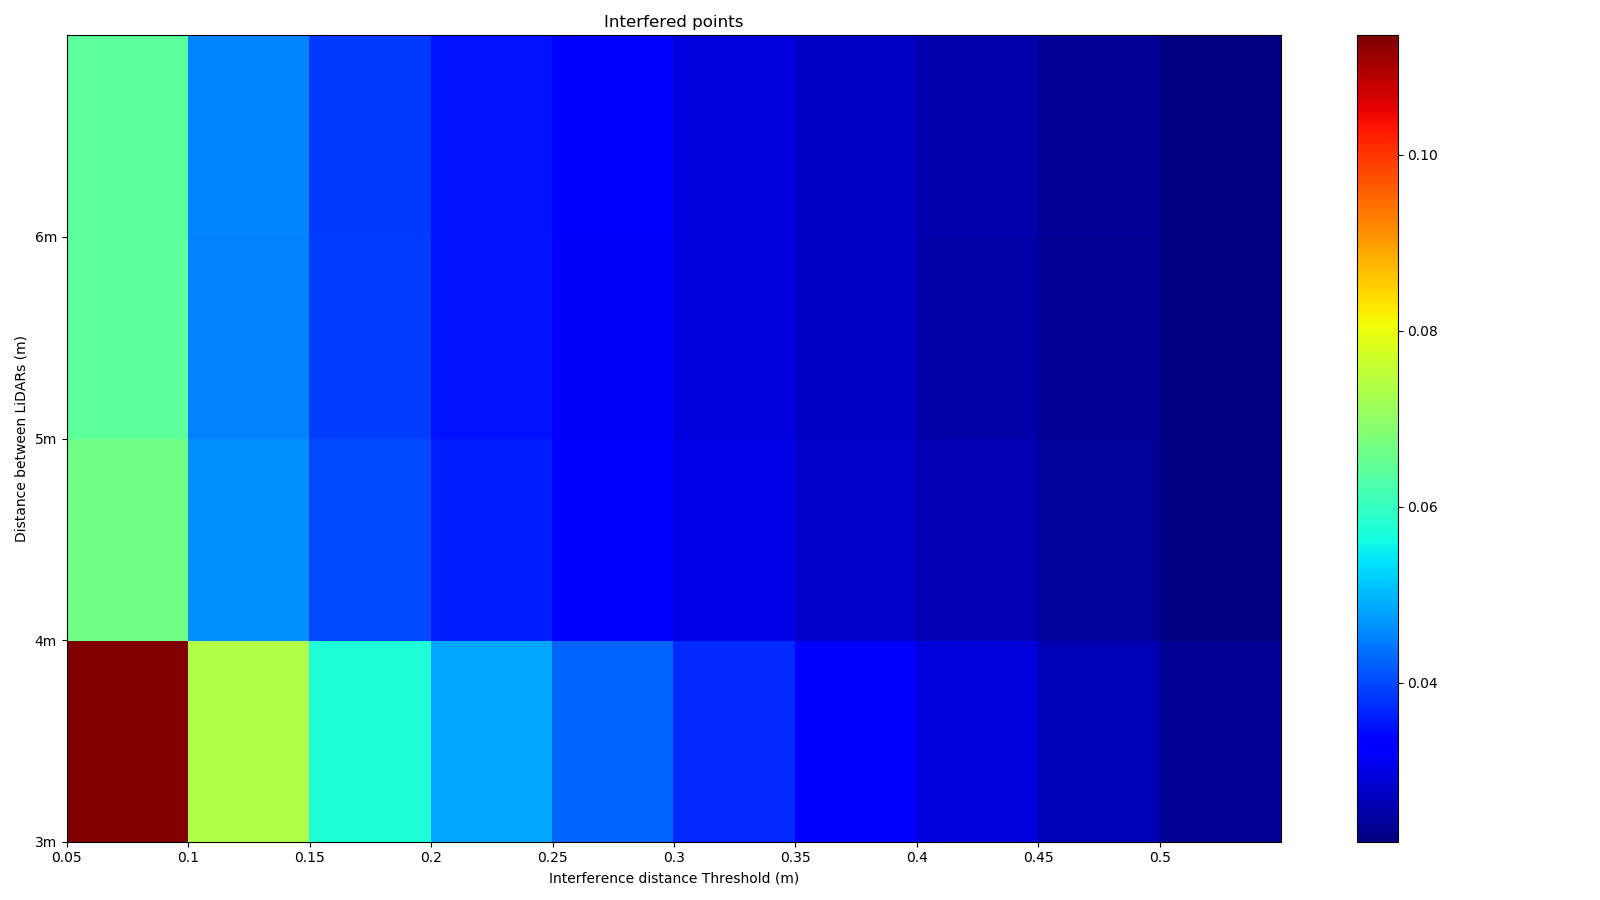
\includegraphics[width=\textwidth]{img/lidar-interference/human/interference_distance_color_mesh.png}
		\caption{}
		\label{fig:human:interference-color-mesh}
	\end{subfigure}
	\qquad
	\begin{subfigure}[c]{0.45\textwidth}
		\centering
		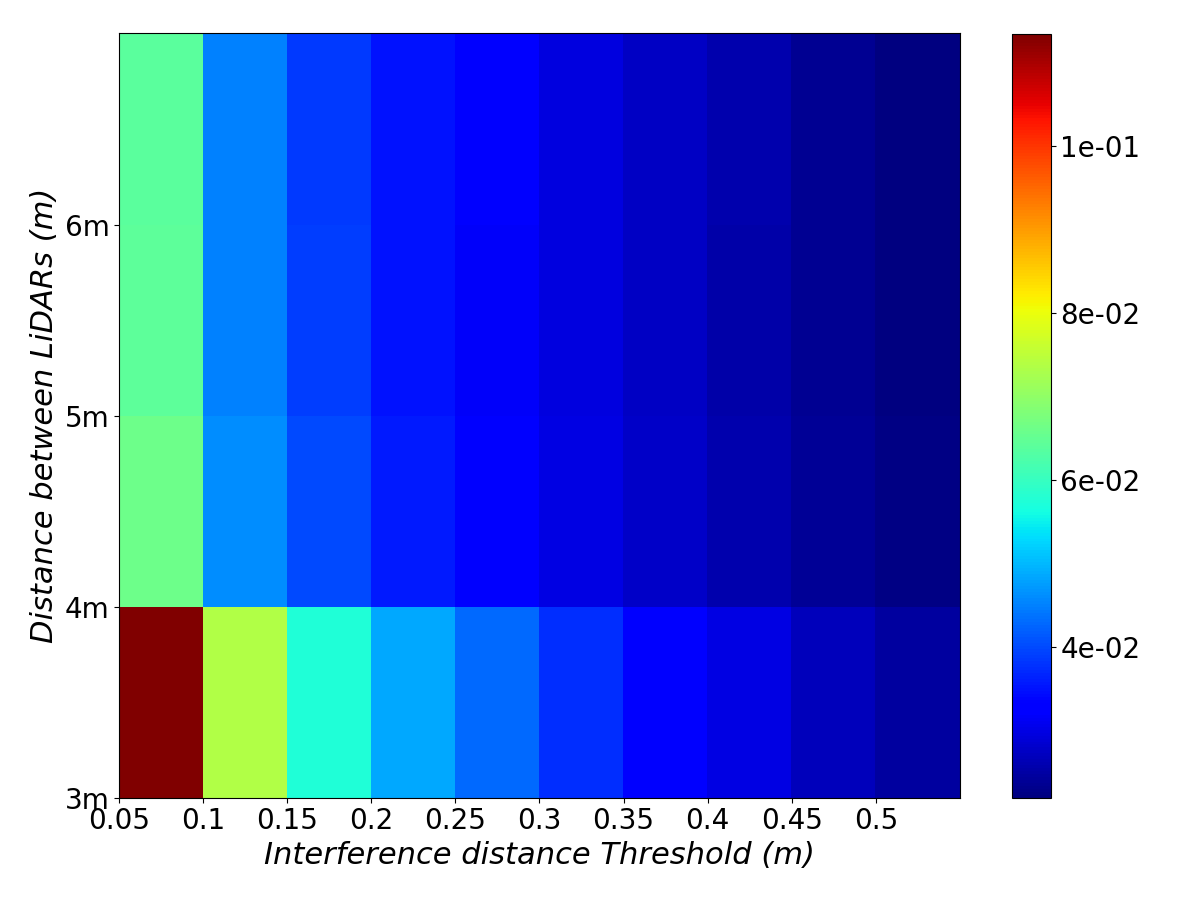
\includegraphics[width=\textwidth]{img/lidar-interference/human/ground_truth_distance_color_mesh.png}
		\caption{}
		\label{fig:human:ground-truth-color-mesh}
	\end{subfigure}
	\\ \vspace{2mm}
	\begin{subfigure}[c]{0.6\textwidth}
		\centering
		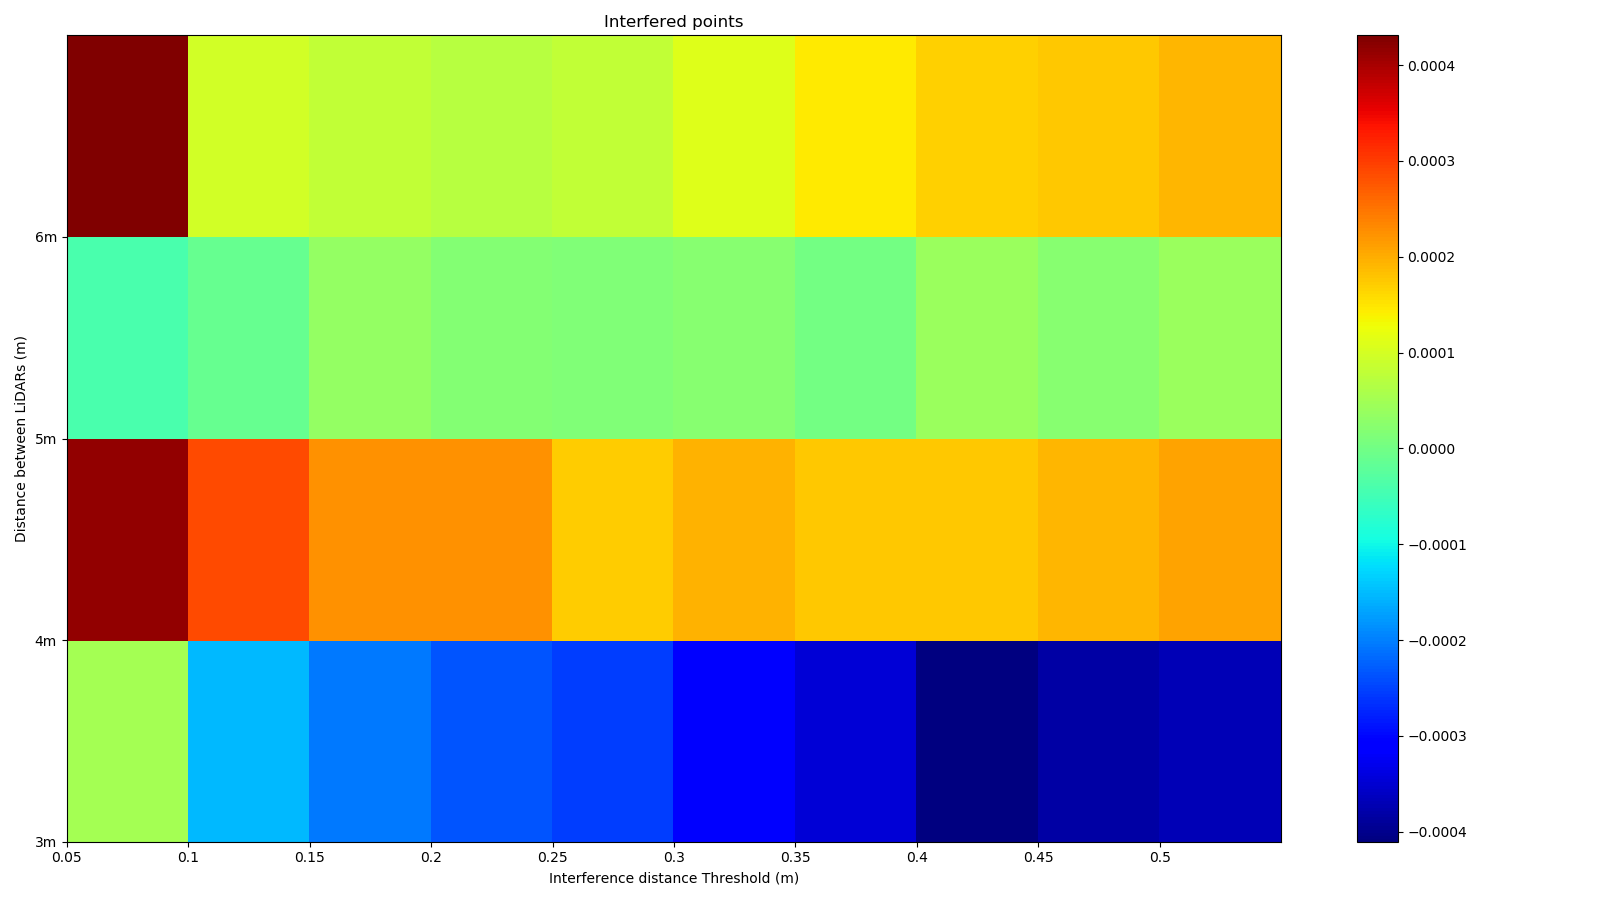
\includegraphics[width=\textwidth]{img/lidar-interference/human/difference_ground_truth_interference_measurement.png}
		\caption{}
		\label{fig:human:difference-color-mesh}
	\end{subfigure}

	\caption[Point-to-Point analysis of the interference on the \textit{Human} dataset without \ac{roi} extraction. Results are presented for the ground-truth bag, interference bag and the subtraction of the results between the two.]{Point-to-Point \ac{lidar} interference analysis on the \textit{Human} dataset without \ac{roi} extraction. In sub-Figure~(\subref{fig:human:interference-color-mesh}), the interfered bag is compared with the ground truth model and in sub-Figure~(\subref{fig:human:ground-truth-color-mesh}), the ground truth bag file is compared with the ground truth model. The latter results are subtracted to the former, resulting in sub-Figure~(\subref{fig:human:difference-color-mesh}). For every sub-figure, the x-axis shows the threshold distance at which a depth difference is considered an interference and the y-axis shows the different values of the distance between the two \acp{lidar}} 
	\label{fig:human:color-mesh}
\end{figure}

Analyzing Figure~\ref{fig:human:color-mesh}, contrary to the results shown in sub-Section~\ref{subsec:lidar-interference:point-to-point-analysis-results}, the distance threshold value does not dominate the interference behavior. The interference decreases with the increasing of the distance between the \acp{lidar} and the distance threshold.

As described in the beginning of sub-Section~\ref{subsec:lidar-interference:point-to-point-analysis-results}, sub-Figures~\ref{fig:human:interference-color-mesh} and~\ref{fig:human:ground-truth-color-mesh} are practically similar. Their subtraction, performed to determine the interference order of magnitude, shown in sub-Figure~\ref{fig:human:difference-color-mesh}, indicates an interference on the order of magnitude of $10^{-4}$. We follow where assumptions on \ac{lidar} measurement noise stated in sub-Section~\ref{subsec:lidar-interference:point-to-point-analysis-results}.

Sub-Figure~\ref{fig:human:difference-color-mesh} shows that, in general, the smooth variation along the x-axis (threshold distance) is contrary to the more abrupt variation on the y-axis (distance between \acp{lidar}). For \SI{3}{\meter}, the subtraction yields negative results, which show that the ground truth model has more errors when compared with the ground truth bag than with the interference bag. For a distance of \SI{5}{\meter}, at which the interferer \ac{lidar} is side by side with the person, the interference is at its minimum, independently of the threshold value. For \SI{4}{\meter} and \SI{6}{\meter}, the interference is at its maximum regardless of the thresholds. 

Since the \acp{lidar}' \ac{los} was never obstructed, direct interference was only changed due to the distance, and we have not observed such behaviors neither in sub-Figure~\ref{fig:distance:difference-color-mesh} nor sub-Figure~\ref{fig:los:difference-color-mesh}. Since direct  \ac{lidar} interference was possible and even with the \acp{lidar} \ac{los} obstructed the behavior does not have any similarities, we can only conclude that the presence of a person (as an obstacle) changes the behavior of the interference, which indicates that besides the more common physical parameters of the setup, such as distance, height, orientation and \ac{los}, there are other parameters, depending on the obstacles positioning on the scene.


\subsubsection{With \ac{roi} Extraction}
With the person placed at (\SI{5.01}{\meter}, \SI{-1.02}{\meter}) on the \ac{lidar} coordinate frame, the distance between the two \acp{lidar} was varied from \SIrange{3}{6}{\meter}, with steps of \SI{1}{\meter}, measured in the same conditions as the distance test (see sub-Section~\ref{subsec:lidar-interference:parameters-under-test} for more details).

Since the maximum distance between any point is \SI{0.5}{\meter}, due to the cluster parameter used (Table~\ref{tab:experimental-euclidian-cluster-specs}), the maximum interference magnitude threshold for the distance on our point-to-point analysis is also \SI{0.5}{\meter}. The starting value is defined as \SI{0.05}{\meter}, with a step of \SI{0.05}{\meter}.

The results of the depth differences between the ground truth model and the interference bag are shown in sub-Figure~\ref{fig:human:roi-interference-color-mesh} and the results of applying the same point-to-point analysis between the ground truth model and the ground truth bag file used to generate the ground truth model are shown in Figure~\ref{fig:human:roi-ground-truth-color-mesh}.

\begin{figure}[!ht]
	\centering
	\begin{subfigure}[c]{0.45\textwidth}
		\centering
		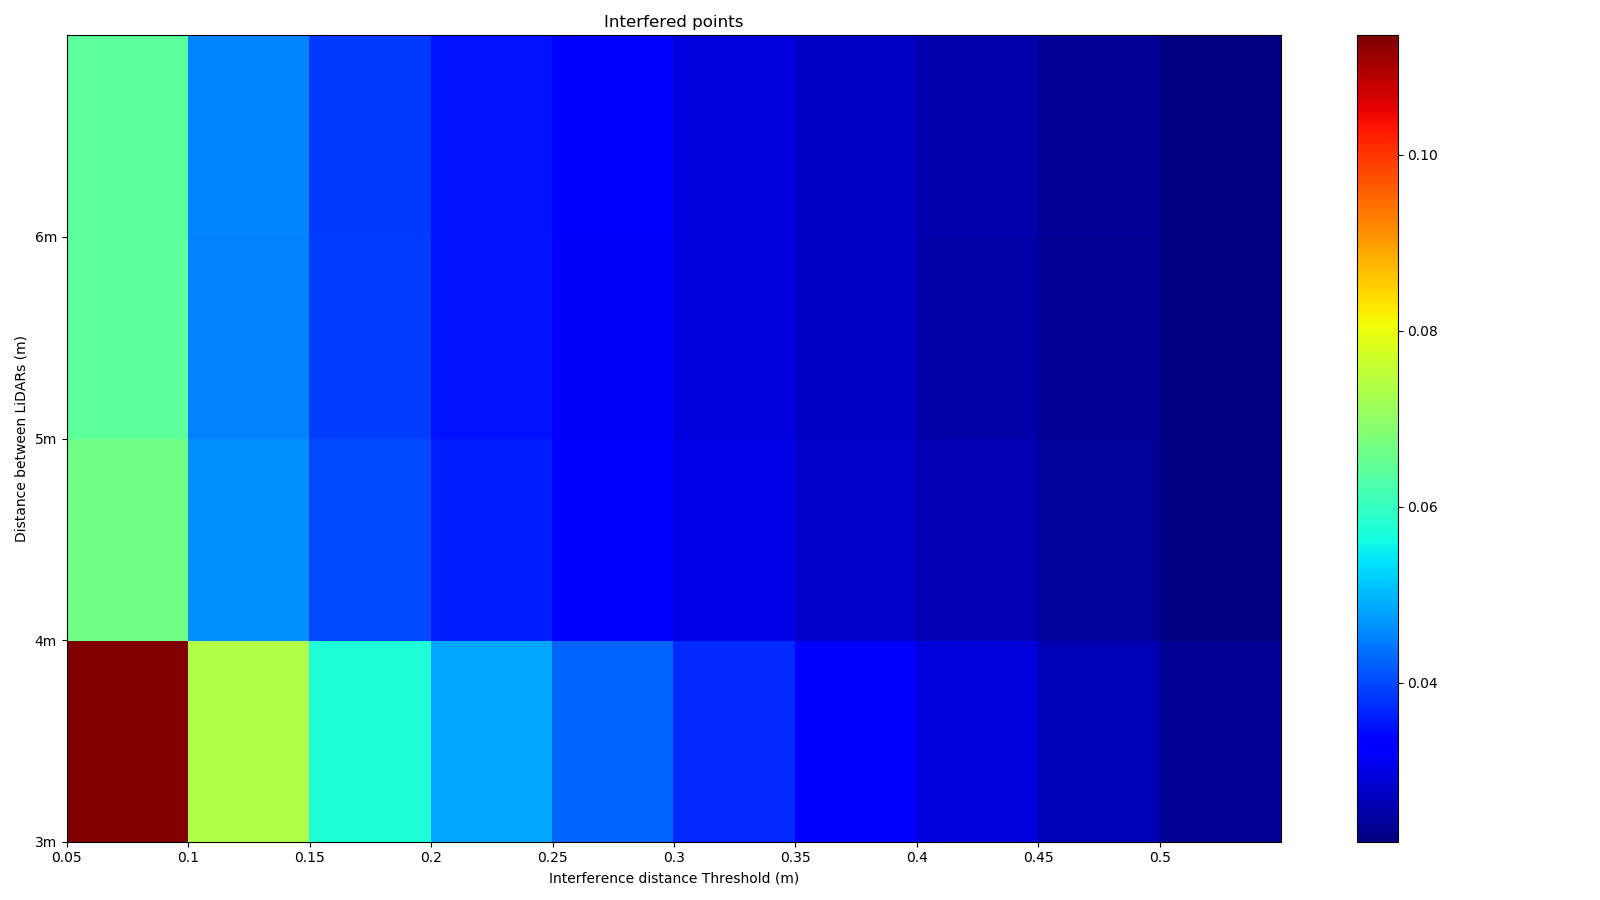
\includegraphics[width=\textwidth]{img/lidar-interference/human/interference_roi_distance_color_mesh.png}
		\caption{}
		\label{fig:human:roi-interference-color-mesh}
	\end{subfigure}
	\qquad
	\begin{subfigure}[c]{0.45\textwidth}
		\centering
		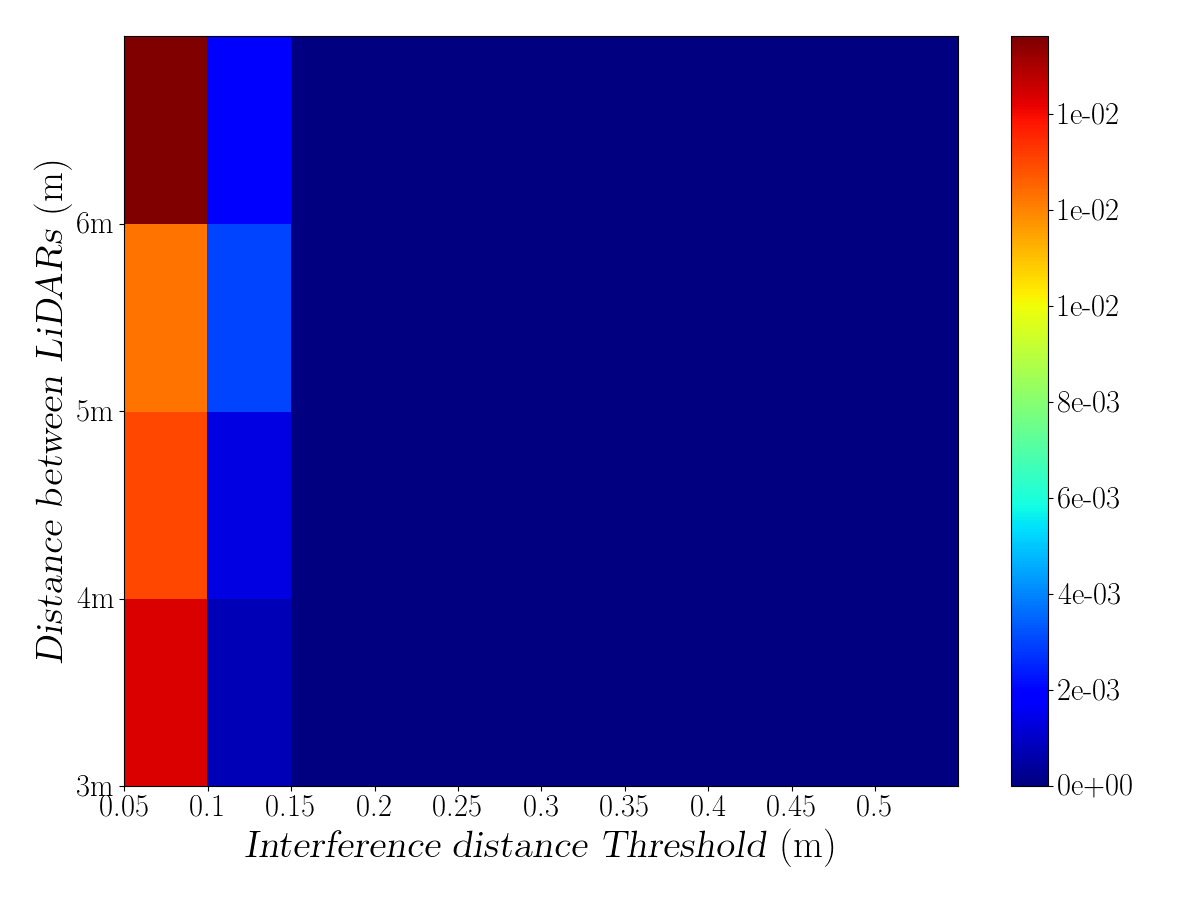
\includegraphics[width=\textwidth]{img/lidar-interference/human/ground_truth_roi_distance_color_mesh.png}
		\caption{}
		\label{fig:human:roi-ground-truth-color-mesh}
	\end{subfigure}
	\\ \vspace{2mm}
	\begin{subfigure}[c]{0.6\textwidth}
		\centering
		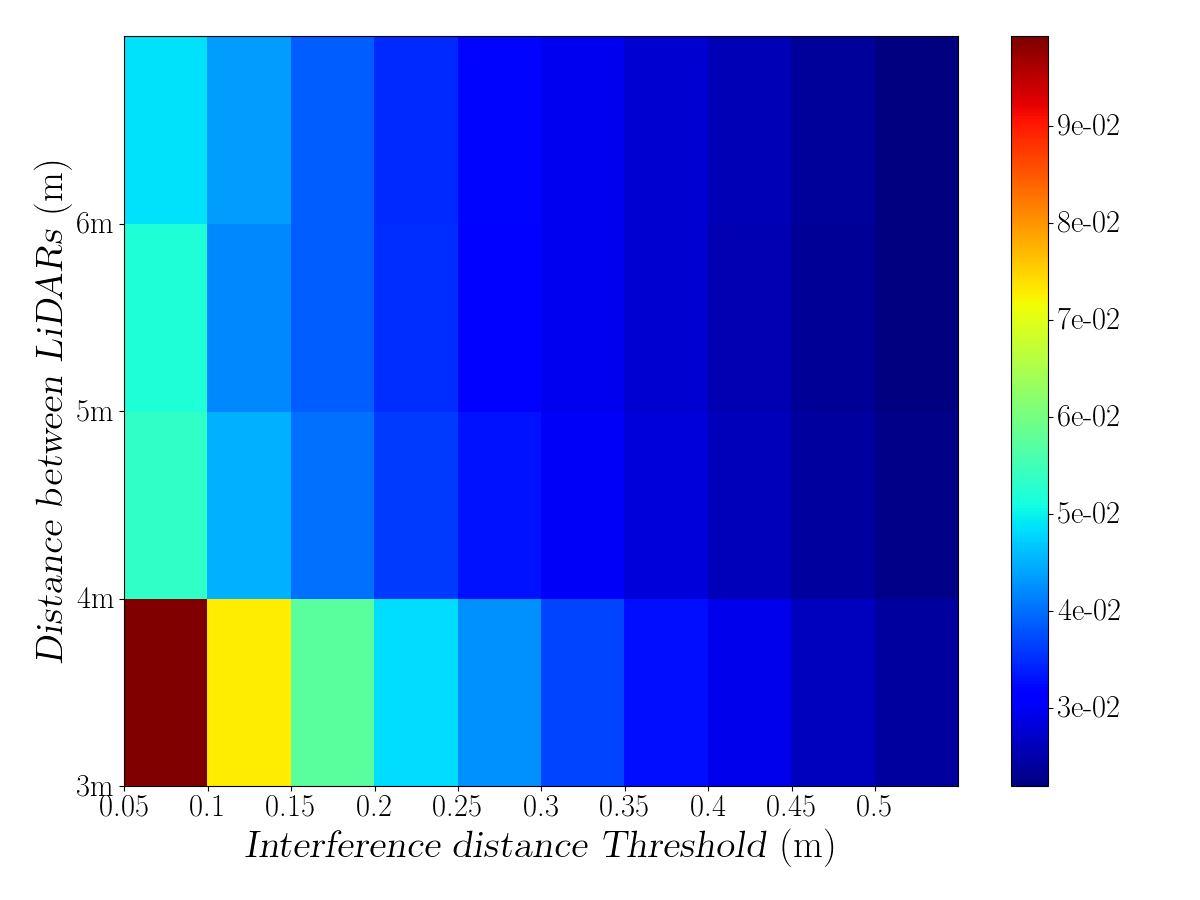
\includegraphics[width=\textwidth]{img/lidar-interference/human/difference_roi_distance_color_mesh.png}
		\caption{}
		\label{fig:human:roi-difference-color-mesh}
	\end{subfigure}

	\caption[Point-to-Point analysis of the interference on the seleced \ac{roi} of the \textit{Human} dataset.]{Point-to-Point \ac{lidar} interference analysis when the parameter under test is the relative distance between the two \acp{lidar}, victim and interferer. In sub-Figure~(\subref{fig:human:roi-interference-color-mesh}), the interfered bag is compared against the ground truth model and in sub-Figure~(\subref{fig:human:roi-ground-truth-color-mesh}), the ground truth bag file is compared with the ground truth model. The latter results are subtracted to the former, resulting in sub-Figure~(\subref{fig:human:roi-difference-color-mesh}). For every sub-figure, the x-axis shows the threshold distance at which a depth difference is considered an interference and the y-axis shows the different values of the distance between the two \acp{lidar}.} 
	\label{fig:human:roi-color-mesh}
\end{figure}

A small residual interference can be observed in Figure~\ref{fig:human:roi-interference-color-mesh} for distance thresholds greater than \SI{0.15}{\centi\meter}. We affirm that this behavior is due to interference since we see no similarities on the analysis of the ground truth bag, in Figure~\ref{fig:human:roi-ground-truth-color-mesh}.

\subsection{Comparison between whole point cloud analysis and \ac{roi} extraction}
In this sub-Section, the same dataset was analyzed using the same algorithms, both for interference analysis and ground truth generation, only differing on the subset of data: the whole point cloud frame or a subset corresponding to a \ac{roi}.

Comparing the ground truth model with the interference bag with and without \ac{roi} extraction (sub-Figure~\ref{fig:human:roi-interference-color-mesh} and sub-Figure~\ref{fig:human:interference-color-mesh}, respectively), one can see that they are quite similar on their behavior and the order of magnitude. Such results indicate that the local behavior of the interference seems to match its global behavior. However, when comparing the ground truth bag with and the \ac{roi} without interference (sub-Figure~\ref{fig:human:roi-ground-truth-color-mesh} and sub-Figure~\ref{fig:human:ground-truth-color-mesh}, respectively), the behavior differs: with \ac{roi} extraction the distance errors measured are one order of magnitude smaller and null after a threshold of \SI{0.15}{\centi\meter}. 

Therefore, the behavior of the subtraction of the interference and ground truth errors is different with and without \ac{roi} extraction (sub-Figure~\ref{fig:human:roi-difference-color-mesh} and sub-Figure~\ref{fig:human:difference-color-mesh}, respectively): while on the former the interference is of an order of magnitude of $10^{-4}$, on the latter is $10^{-2}$. The distance at which the interference is maximum (\SI{4}{\meter} and \SI{6}{\meter}) or minimum (\SI{5}{\meter}) is not present when \ac{roi} extraction is done. The analysis on the extracted \ac{roi} is also more ``well-behaved'': the number of errors is maximum when the \acp{lidar} are closer and the threshold is smaller; and is minimum when the \acp{lidar} are further away and the threshold is maximum, with smooth transitions on both axis between the two extremes.

When comparing point clouds with and without \ac{roi} extraction, caution must be taken before  ``jumping'' to conclusions. \acp{roi} contains fewer points when compared with the whole point cloud: 128.4 and 26243.2, on average, respectively. Since \ac{roi} filtering removes points that are not aligned with the object of interest, the outliers described in sub-Section~\ref{subsec:object-detection:projection-correspondences} are filtered out; clustering removes points that are not near the object of interest position on the \ac{lidar} coordinate frame, including severe interference and the outliers aligned with the \ac{roi} direction, analyzed in sub-Section~\ref{subsec:lidar-interference:room-outliers-experimental-setup}.

Preliminary conclusions from such a small dataset on \ac{roi} interference analysis (we only tested for 4 distances, in the same environment, with the same object of interest), show that extracting \acp{roi} of the clustering reduces the noise associated to the ground-truth model generation and shows that, on the conditions of our scenario, the relative interference on an object of interest is higher than on the entire point cloud. Such conclusions could undermine the possibility of point cloud object detection, as we assume, since the level of interference, due to the reduced number of points, is greater.

We postulate the hypothesis that \ac{lidar} noise plays a dominant role on regions of the point with reduced features of interest, whereas the impact of interference becomes significant on \acp{roi}. Such hypothesis was not tested and it is left for future work.


\section{Comparison with the \acl{sota}}
\label{sec:lidar-interference:sota-comparison}
Despite the experimental setups being quite different, since ours uses a multi-beam tridimensional \ac{lidar} and Kim's\etal and Popko's\etal using a single beam two-dimensional \ac{lidar}, we attempt to establish comparisons between our results and theirs.

Popko's\etal repeats Kim's\etal setups, and they have 4 experimental setups: two \textit{Side-by-Side} configurations, one for maximizing direct interference (\textit{Face-to-Face}) and another to minimize it and study scattered interference, \textit{Back-to-Back}. The test scenarios can be seen in Figure~\ref{fig:kim-setups}. 

Establishing parallelisms with ours, \textit{Distance} test scenario is a good candidate for \textit{Face-to-Face} and our \textit{\ac{lidar} \ac{los} Obstruction} a good candidate to be evaluated against \textit{Back-to-back}. All the other test scenarios, except for \textit{\ac{lidar} \ac{los} Obstruction}, can be used to compare with Kim's\etal and Popko's\etal \textit{Side-by-Side} results. However, since the main objective of these results is to study the impact of the \ac{fov} between the two \acp{lidar}, on situations when they do not detect each other, no comparisons will be made for \textit{Side-by-Side} study.


During this comparison we will not consider the interfered lines metric, since in our opinion, it is not relevant to understand interference and might be misleading, since on our case, a single error on a line of $\approx 1800$ points will result on an interfered line. Table~\ref{tab:kim-vs-ours-comparison} shows the results of Kim's\etal setups versus ours. Since only one of Popko's\etal setups has experimental quantitative measurements: \textit{Side-by-Side \#1} with 1.04\% of interference, it is not possibility to compare with ours' and Kim's\etal.


\begin{table}[!ht]
	\vspace{6mm}
	\centering
	\renewcommand{\arraystretch}{1.3}
	\begin{tabular}{@{}p{7.5cm}cc@{}}
			\toprule
			\multirow{2}{*}{Experimental Setup Codename} & \multicolumn{2}{c}{Relative Frequence of Interfered Points} \\ \cmidrule{2-3}
																									 & Kim's\etal & Our's\\
			\midrule
			\textit{Face-to-Face} vs. \textit{Distance}   & $2.583\E^{-5}$  & $\approx 10^{-4}$ \\ \midrule
			\textit{Back-to-Back A} vs. \textit{\ac{lidar} \ac{los} Obstruction}  & $3.387\E^{-6}$ & \multirow{2}{*}{$\approx 10^{-6}$} \\
			\textit{Back-to-Back B} vs. \textit{\ac{lidar} \ac{los} Obstruction} & $3.514\E^{-6}$ & \\ \bottomrule
		\end{tabular}
		\caption[Comparison of Kim's\etal interferference with our results for equivalent setups.]{Comparison of Kim's\etal setups interference measurements with our equivalent setups.}
		\label{tab:kim-vs-ours-comparison}
\end{table}

When the \acp{lidar} can interfere directly, i.e, there are no objects in between, our measurement of interference is higher than Kim's\etal by one degree of magnitude. We can justify that difference since on Kim's setup the two \acp{lidar} have their laser aligned at polar angle of \SI{0}{\degree} and VLP-16 and Pandar40 have more lasers oriented on another directions, with the VLP-16 not having a laser placed at a polar angle of \SI{0}{\degree}. Comparing \textit{Back-to-Back} tests with our \textit{\ac{lidar} \ac{los} Obstruction}, the results are on the same order of magnitude, revealing that the impact of scatter interference between \ac{lidar}'s, even if comparing a scanner with only one line to one with 16, remain similar. Popko's\etal results do not match ours or Kim's results, with 1.04\% of relative number of interferer points in scenario \textit{Side-by-Side \#1}.

\section{Final Remarks}
For all the data presented, there are two considerations that are not addressed:

\begin{itemize}
	\item We have no information about the likeliness of direct \ac{lidar} interference saturating the detector of the victim's \ac{lidar}. If such behavior is possible, it may or may not be considered a valid measurement by the hardware, and may or may not be discarded by the device driver firmware before being accessible by the user;
	\item The \ac{lidar}'s hardware and the driver firmware impose a maximum limit to the distance at which a point can be measured. Therefore, we have no way of count the points that span beyond the limit of the \ac{lidar} measurement distance. 
\end{itemize}

Our experiments led us to tinkering about these problems, but no action was taken to address them.
